\documentclass[11pt,a4paper]{article}

% ---------------------------------------------------------------------------
% Paquetes
% ---------------------------------------------------------------------------
\usepackage[utf8]{inputenc}
\usepackage[T1]{fontenc}
\usepackage[spanish,es-tabla]{babel}
\usepackage[scaled]{helvet}
\renewcommand{\familydefault}{\sfdefault}
\usepackage[margin=2.5cm]{geometry}
\usepackage{graphicx}
\usepackage{booktabs}
\usepackage{array}
\usepackage{caption}
\usepackage{enumitem}
\usepackage{xcolor}
\usepackage[colorlinks=true,linkcolor=black,citecolor=black,urlcolor=blue]{hyperref}
\usepackage{titlesec}
\usepackage{setspace}
\usepackage{listings}

\lstdefinestyle{python}{
  basicstyle=\ttfamily\scriptsize,
  keywordstyle=\bfseries,
  commentstyle=\itshape\color{gray},
  stringstyle=\color{gray},
  showstringspaces=false,
  breaklines=true,
  breakatwhitespace=false,
  frame=single,
  framesep=4pt,
  xleftmargin=2pt,
  xrightmargin=2pt,
  tabsize=4,
  language=Python,
  columns=fullflexible,
}
\lstset{style=python}
\renewcommand{\lstlistingname}{Código}
\lstset{
  literate=
   {á}{{\'a}}1 {é}{{\'e}}1 {í}{{\'i}}1 {ó}{{\'o}}1 {ú}{{\'u}}1
   {Á}{{\'A}}1 {É}{{\'E}}1 {Í}{{\'I}}1 {Ó}{{\'O}}1 {Ú}{{\'U}}1
   {ñ}{{\~n}}1 {Ñ}{{\~N}}1 {ü}{{\"u}}1 {º}{{\textordmasculine}}1
}

\setstretch{1.06}
\setlength{\parskip}{0.4em}
\setlength{\parindent}{0pt}

\titleformat{\section}{\normalfont\Large\bfseries}{\thesection.}{0.5em}{}
\titleformat{\subsection}{\normalfont\large\bfseries}{\thesubsection.}{0.5em}{}
\titlespacing*{\section}{0pt}{1.3em}{0.5em}
\titlespacing*{\subsection}{0pt}{0.9em}{0.35em}

% ---------------------------------------------------------------------------
% Portada
% ---------------------------------------------------------------------------
\begin{document}

\begin{titlepage}
\centering
\vspace*{1.5cm}

{\large Universidad Complutense de Madrid}\\[0.3cm]
{\large Máster en Big Data, Data Science e Inteligencia Artificial}\\[2.5cm]

{\Huge \bfseries Predicción y explicación de la gravedad de accidentes de tráfico en Madrid}\\[0.6cm]
{\Large Un enfoque dual para triaje operativo y prevención vial}\\[2.5cm]

{\large Trabajo Fin de Máster}\\[2cm]

\begin{tabular}{rl}
\textbf{Autora:} & Meritxell Abellan Collado \\[0.3cm]
\textbf{Tutores:} & Carlos Ortega \\
 & Santiago Mota \\
\end{tabular}

\vfill
{\large Septiembre 2026}

\end{titlepage}

\tableofcontents
\newpage

\listoffigures
\newpage

% =============================================================================
\section{Introducción}
% =============================================================================

\subsection{Contexto y motivación}

Los accidentes de tráfico son una de las principales causas de mortalidad evitable en entornos urbanos. Madrid, como una de las ciudades con mayor volumen de tráfico de España, registra miles de accidentes al año con niveles de gravedad muy dispares --- desde ilesos hasta heridos graves y fallecidos. Anticipar qué factores incrementan el riesgo de un desenlace grave tiene valor tanto operativo (priorización de recursos de emergencia) como preventivo (diseño de campañas de seguridad vial dirigidas).

Este trabajo utiliza el conjunto de datos abiertos de accidentalidad del Ayuntamiento de Madrid correspondiente al periodo 2012--2018, con información a nivel de persona implicada (conductor, pasajero o peatón) para cada accidente registrado. Es un dataset real, de publicación pública, con los defectos de calidad de dato habituales de una fuente administrativa --- valores sin asignar, inconsistencias de formato, duplicados de exportación--- que se auditan y documentan de forma explícita a lo largo del trabajo.

\subsection{Dos preguntas de investigación}

El trabajo aborda dos preguntas complementarias, que comparten el mismo dataset y la misma variable objetivo (gravedad del accidente: grave/mortal frente a leve/ileso) pero difieren en qué información pueden utilizar y para qué se orienta el resultado:

\begin{itemize}
\item \textbf{Pregunta 1 --- Triaje operativo:} ¿es posible anticipar, con la información disponible en el momento del aviso de un accidente (ubicación, momento, condiciones meteorológicas, tipo de vía y tipo de siniestro), la probabilidad de que resulte grave, con el fin de apoyar la priorización de los recursos de emergencia --- SAMUR, Policía Municipal, Bomberos--- que se despachan a través del 112 tras la llamada?
\item \textbf{Pregunta 2 --- Prevención vial:} ¿qué factores --- lugar, tipo de siniestro, perfil de las personas implicadas... --- se asocian con una mayor gravedad, con el fin de informar campañas de prevención vial dirigidas (por ejemplo, focalizadas en distritos concretos, franjas horarias de mayor riesgo o colectivos de edad más vulnerables)?
\end{itemize}

Estas dos preguntas no son intercambiables. La Pregunta 1 exige que toda variable esté disponible en el momento del aviso: un modelo que use el perfil demográfico exacto de los implicados no podría desplegarse nunca para decidir cuántos recursos enviar, por bien que prediga en retrospectiva. La Pregunta 2 no tiene esa restricción, y precisamente en ese perfil reside gran parte de la señal más útil para la prevención (por ejemplo, qué rangos de edad concentran más riesgo). Por eso se construyen dos modelos con propósitos distintos, evaluados con criterios distintos, sobre dos matrices de variables distintas construidas a partir del mismo dataset base.

\subsection{Objetivos específicos}

\begin{enumerate}[nosep]
\item Caracterizar mediante análisis exploratorio los patrones de gravedad de los accidentes de tráfico en Madrid según variables de lugar, tiempo, tipo de siniestro y perfil de las personas implicadas.
\item Construir un \textbf{modelo de triaje operativo}, entrenado únicamente con variables disponibles en el momento del aviso, y evaluar su capacidad de discriminación y calibración como apoyo a la priorización de recursos.
\item Construir un \textbf{modelo explicativo}, con todas las variables disponibles a posteriori, para identificar los factores de riesgo más relevantes mediante técnicas de interpretabilidad.
\item Cuantificar la diferencia de rendimiento entre ambos modelos, como medida explícita de cuánto se ``pierde'' por restringirse a la información disponible en el momento del aviso.
\item Traducir los hallazgos del modelo explicativo en recomendaciones concretas de focalización geográfica, temporal y demográfica para campañas de prevención vial.
\item Llevar el modelo de triaje más allá del entorno de notebook, mediante un pipeline reutilizable y una aplicación funcional de demostración.
\end{enumerate}

Más allá de aplicar un conjunto de algoritmos estándar sobre datos ya limpios, el trabajo pone el énfasis en las decisiones metodológicas que determinan si esos resultados son fiables:

\begin{itemize}[nosep]
\item Disponibilidad temporal entre las dos preguntas;
\item Detección y corrección de pseudo-replicación estadística en el análisis exploratorio;
\item Verificación explícita de los supuestos de cada test antes de confiar en su resultado;
\item Ingeniería de variables que evita fugas de información y trampas de colinealidad conocidas;
\item Validación por deriva temporal del propio periodo de prueba;
\item Contraste cruzado de los hallazgos de interpretabilidad con un segundo modelo de naturaleza distinta.
\end{itemize}

Cada una de estas decisiones se documenta con su justificación en las secciones siguientes.

% =============================================================================
\section{Datos y análisis exploratorio}
% =============================================================================

\subsection{El dataset}

El conjunto de datos original contiene 199.078 registros a nivel de persona implicada, correspondientes a 68.773 accidentes únicos ocurridos en Madrid entre el 1 de enero de 2012 y el 31 de diciembre de 2018 en los 21 distritos de la ciudad. Las variables se agrupan en siete bloques: identificación del accidente y la persona; tiempo (fecha, franja horaria, día de la semana); lugar (distrito, descripción libre de la vía); condiciones atmosféricas y estado del firme (doce columnas binarias); tipo de siniestro; perfil de la persona (sexo, tramo de edad, tipo de vehículo, rol); y la variable de interés, la lesividad sufrida por cada implicado (ilesa, herida leve, herida grave o fallecida).

\subsection{Analisis de duplicados}

Se auditó la presencia de duplicados en dos niveles:

\begin{itemize}[nosep]
\item 4.065 filas exactamente idénticas en todas sus columnas (2,33\,\% del total tras excluir testigos). Coincidir por azar en absolutamente todas las variables --- vehículo, lesividad, tramo de edad, sexo--- es prácticamente imposible, así que se interpretan como errores de exportación y se eliminan.
\item 1.252 registros con el mismo perfil demográfico (mismo accidente, tipo de persona, sexo, tramo de edad y lesividad) pero que difieren en alguna otra columna. Al no poder descartarse que sean personas distintas con un perfil parecido, se documentan como limitación de calidad del dato pero no se eliminan.
\end{itemize}

Este criterio --- corregir solo lo estadísticamente insostenible, documentar el resto--- se mantiene en todo el trabajo.

Tras excluir los 24.725 testigos (que no son implicados con lesividad propia y no aportan señal para el objetivo) y los duplicados exactos, el dataset de trabajo a nivel persona queda en 170.288 registros.

\subsection{La variable objetivo}

La variable de gravedad se agrega a nivel accidente como el máximo de lesividad entre todos sus implicados: un accidente se considera \textbf{grave} si al menos una persona resultó herida grave o fallecida, y \textbf{leve} en caso contrario. 
Antes de tomar esta decisión se investigó si la falta de asignación de lesividad (3,78\,\% de los registros de persona) es aleatoria. El desglose muestra que no lo es: por año oscila de forma estable entre el 3,17\,\% y el 5,18\,\%, y por distrito entre el 3\,\% y el 5,12\,\% sin diferencias relevantes, pero por tipo de accidente el rango es mucho más amplio (2,14\,\% a 17,16\,\%), concentrándose de forma marcada en los choques contra objetos fijos (17,16\,\%) y las caídas de vehículos de tres ruedas (16,67\,\%) --- entre cuatro y ocho veces más que el resto de tipos.

Este patrón podría haber sesgado el target si se hubiera mantenido tras agregar a nivel accidente, así que se comprobó el impacto real: de los 68.773 accidentes registrados, ninguno se pierde por completo, porque siempre queda al menos un implicado con lesividad conocida. El riesgo residual --- que la persona sin lesividad asignada fuera la más gravemente herida y el accidente quede infravalorado--- se estimó en un 1,7\,\% del dataset. Como segunda comprobación, independiente de la primera, se comparó el número de víctimas declarado en el propio dataset con el recuento real de heridos y fallecidos por accidente, encontrando un desajuste del 1,44\,\% --- del mismo orden de magnitud que el riesgo estimado, y coherente con la hipótesis de que se explica por personas con lesividad no asignada que sí eran víctimas, no por un error de captura de otra naturaleza.

El resultado es un fuerte desequilibrio de clases: a nivel accidente, solo el 9,60\,\% resultan graves (ratio aproximado 9,4:1); a nivel persona, el desequilibrio es aún mayor (4,31\,\%, ratio 22,2:1), porque un mismo accidente grave puede implicar a varias personas ilesas. Este desequilibrio condiciona toda la fase de modelización: la métrica de referencia no puede ser la exactitud (\emph{accuracy}), que con un clasificador que predijera siempre ``no grave'' ya alcanzaría un 90,4\,\%, sino medidas que tienen en cuenta el desequilibrio, como el área bajo la curva ROC y bajo la curva precisión-recall.

\subsection{Perfil de los implicados}

\begin{itemize}[nosep]
\item \textbf{Rol:} los conductores son el más frecuente (72\,\%), pero los peatones concentran la mayor proporción de heridos graves y fallecidos --- el colectivo más vulnerable.
\item \textbf{Sexo:} los hombres registran más volumen de accidentalidad que las mujeres, con gravedad relativa similar.
\item \textbf{Edad:} mayores de 65 y menores de 18 muestran la mayor gravedad relativa; los tramos de 25 a 44 años concentran el mayor volumen, por ser los conductores más activos.
\item \textbf{Vehículo:} motocicletas y bicicletas tienen la mayor tasa de lesividad grave (figura~\ref{fig:lesividad_vehiculo}); los turismos concentran el mayor volumen absoluto.
\end{itemize}

Un 18\,\% de los registros de persona no tiene tipo de vehículo asignado, pero no es un problema de calidad sino estructural: el 99,94\,\% de los peatones no tiene vehículo (lógico, un peatón no conduce ninguno), mientras que conductores y viajeros tienen el dato casi completo.

\begin{figure}[h]
\centering
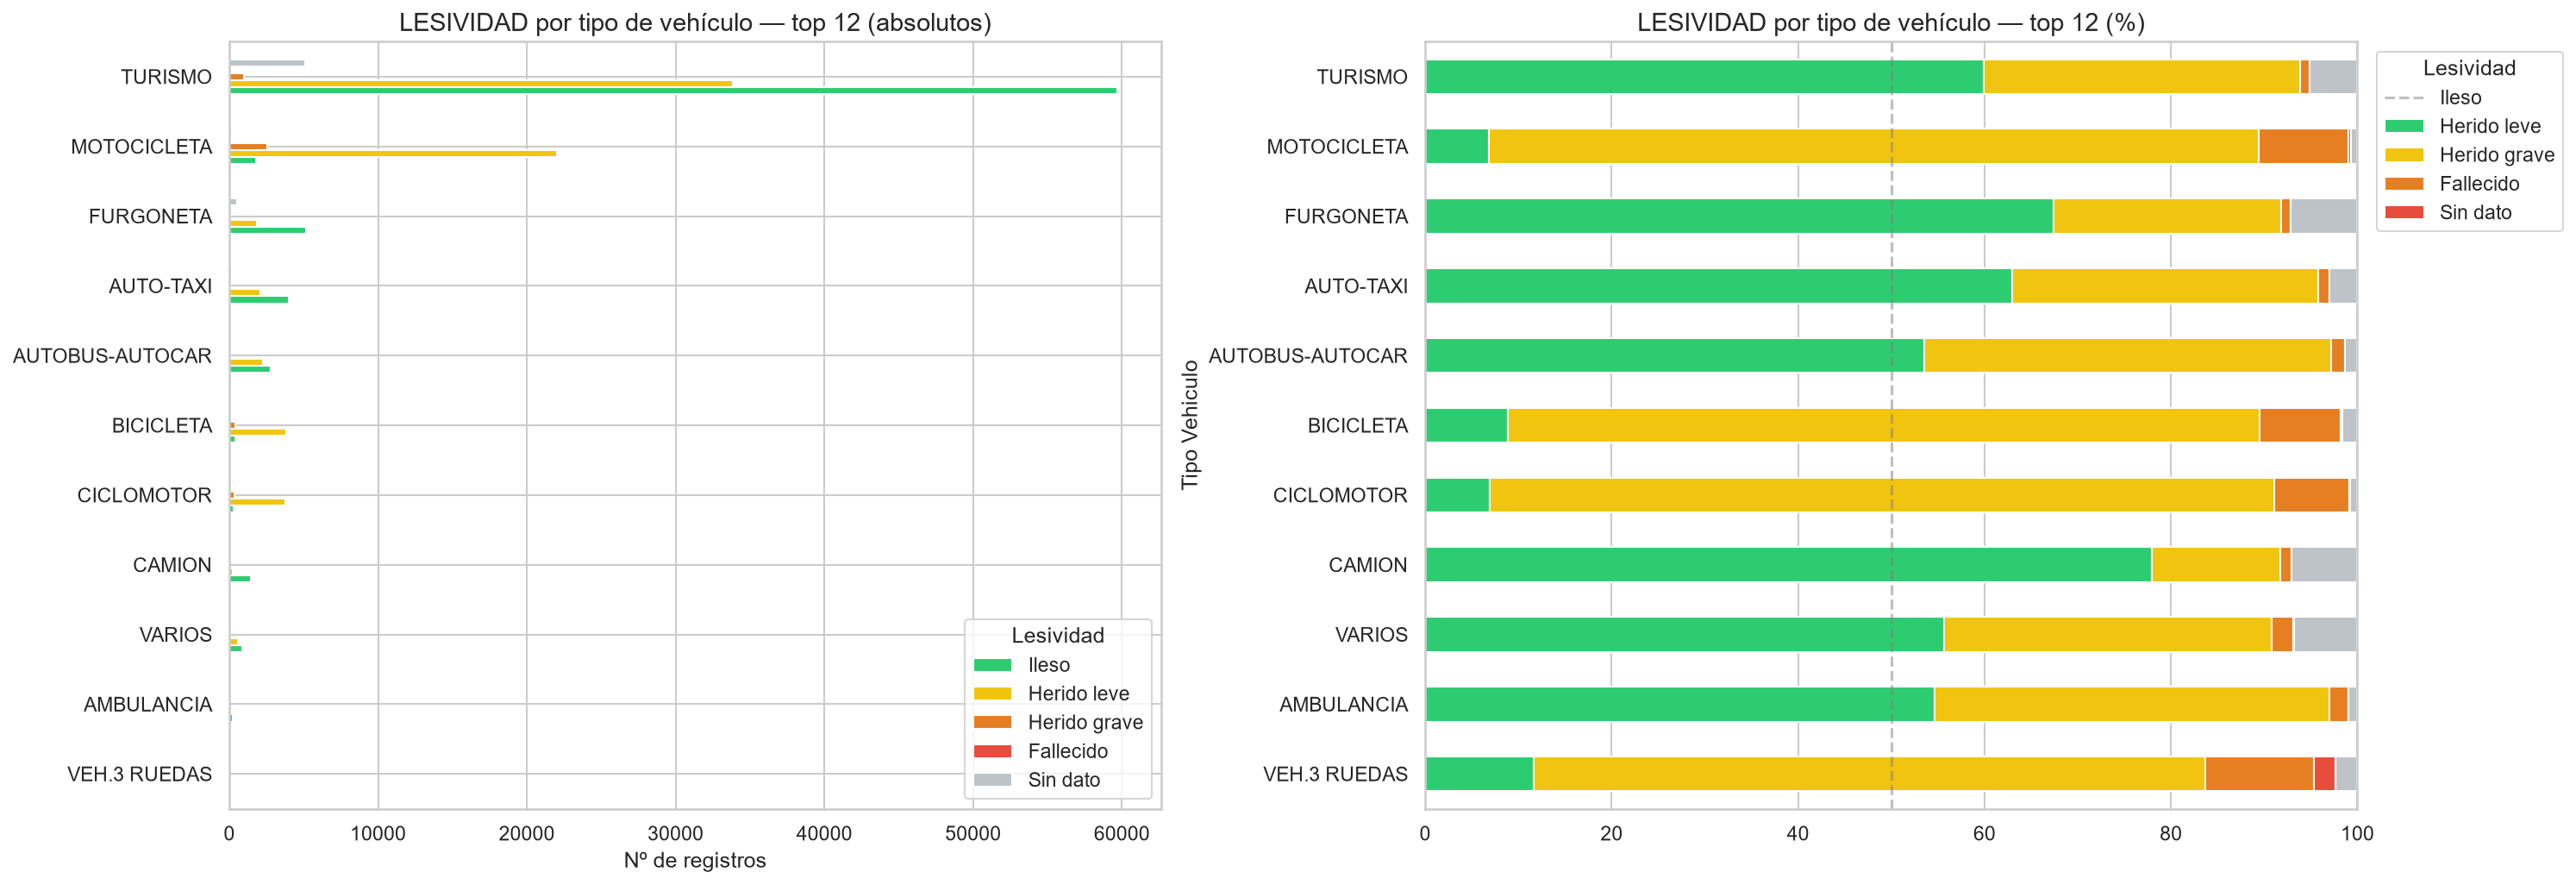
\includegraphics[width=0.95\textwidth]{../figures/13_lesividad_por_vehiculo.png}
\caption{Distribución de lesividad por tipo de vehículo (valores absolutos y \%). Motocicletas, bicicletas y ciclomotores destacan por su proporción de heridos graves y fallecidos frente al turismo, pese a un volumen absoluto mucho menor.}
\label{fig:lesividad_vehiculo}
\end{figure}

\subsection{Análisis temporal}

Como la variable objetivo es la gravedad y no el volumen, el cruce más relevante de esta sección es la tasa de HG+MT por día y franja horaria (figura~\ref{fig:heatmap_gravedad}): la madrugada --- especialmente de 2h a 6h, y con mayor intensidad los fines de semana--- destaca de forma consistente sobre el resto de horas. Es un patrón puramente descriptivo en esta fase, que la Sección~\ref{sec:focalizacion} confirma después de forma independiente con SHAP y regresión logística.

\begin{figure}[h]
\centering
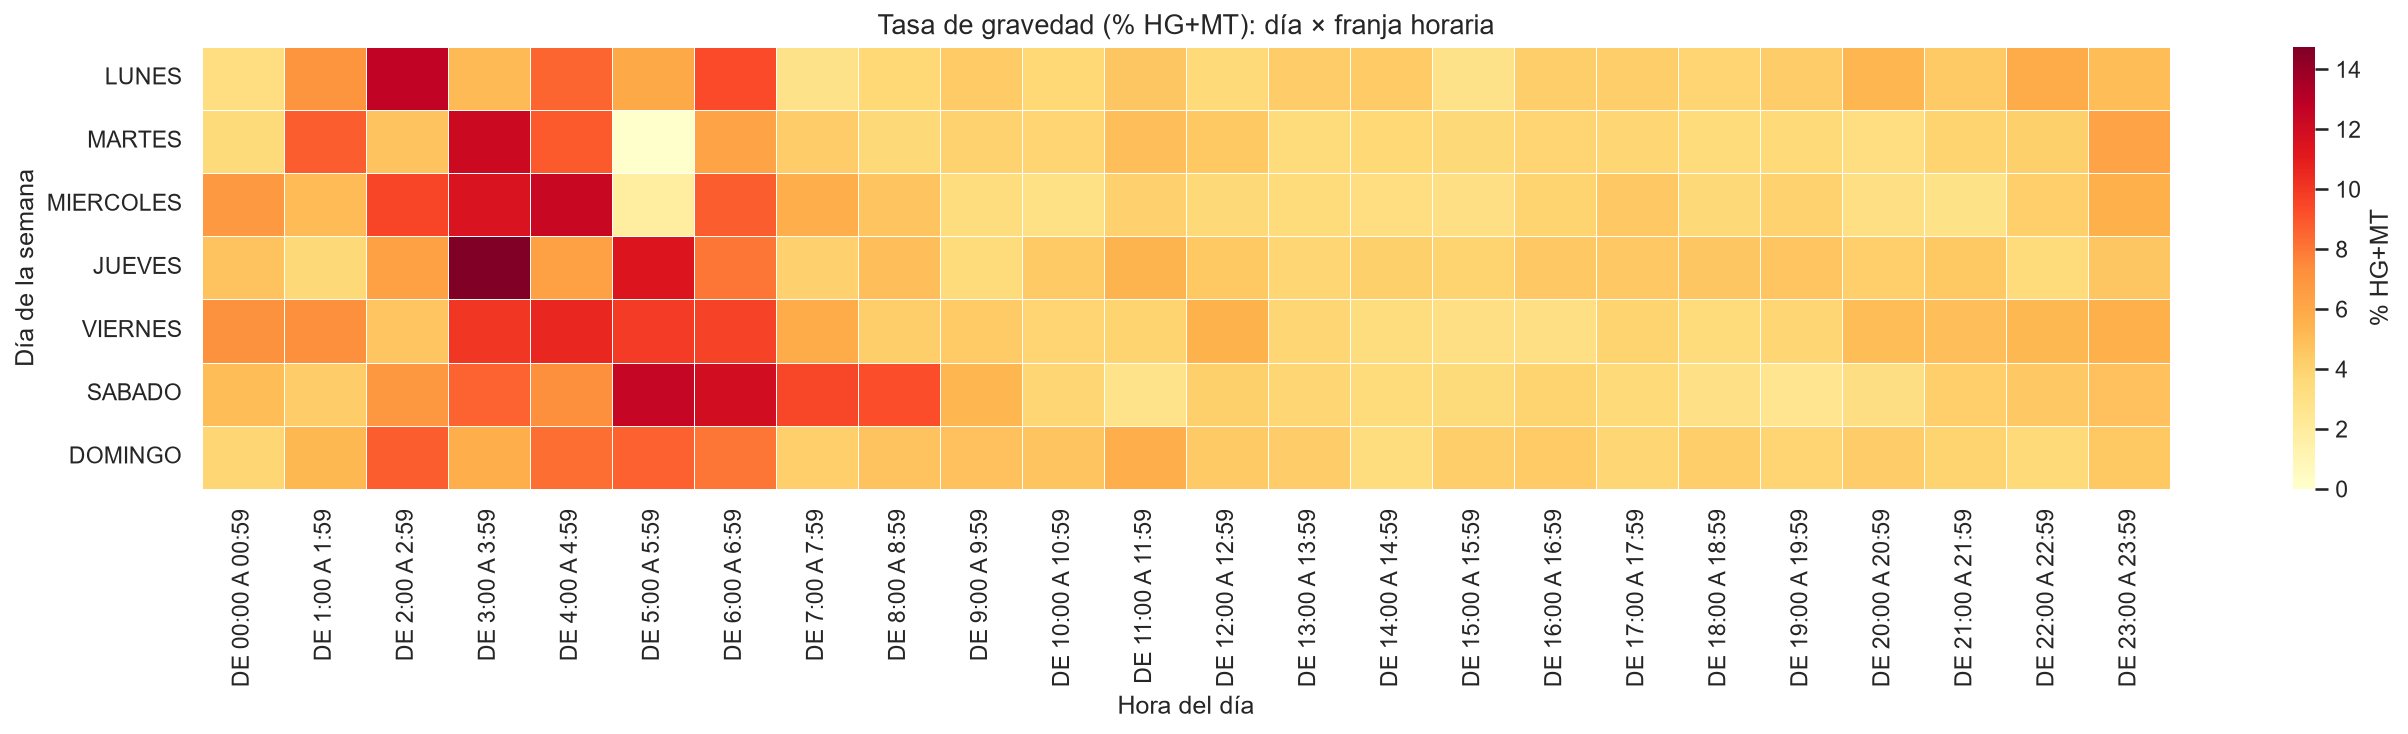
\includegraphics[width=0.8\textwidth]{../figures/07e_heatmap_gravedad_dia_hora.png}
\caption{Mapa de calor de la tasa de gravedad (\% HG+MT) por día de la semana y franja horaria.}
\label{fig:heatmap_gravedad}
\end{figure}

Por volumen, en cambio, el patrón es justo el opuesto: el número de accidentes crece a lo largo del periodo, con estacionalidad clara (octubre, noviembre y junio concentran más accidentalidad; julio y agosto, menos, probablemente por el tráfico vacacional), los días laborables superan al fin de semana, y las horas punta (9h, 14h, 17h) son las de mayor volumen --- el cruce de día y franja horaria por volumen (figura~\ref{fig:heatmap}) señala su punto máximo el viernes entre las 14h y las 16h, precisamente la franja opuesta a la madrugada de mayor riesgo. Se incluye como contraste: la madrugada es una franja de bajo volumen pero alta gravedad, y el viernes tarde, lo contrario.

\begin{figure}[h]
\centering
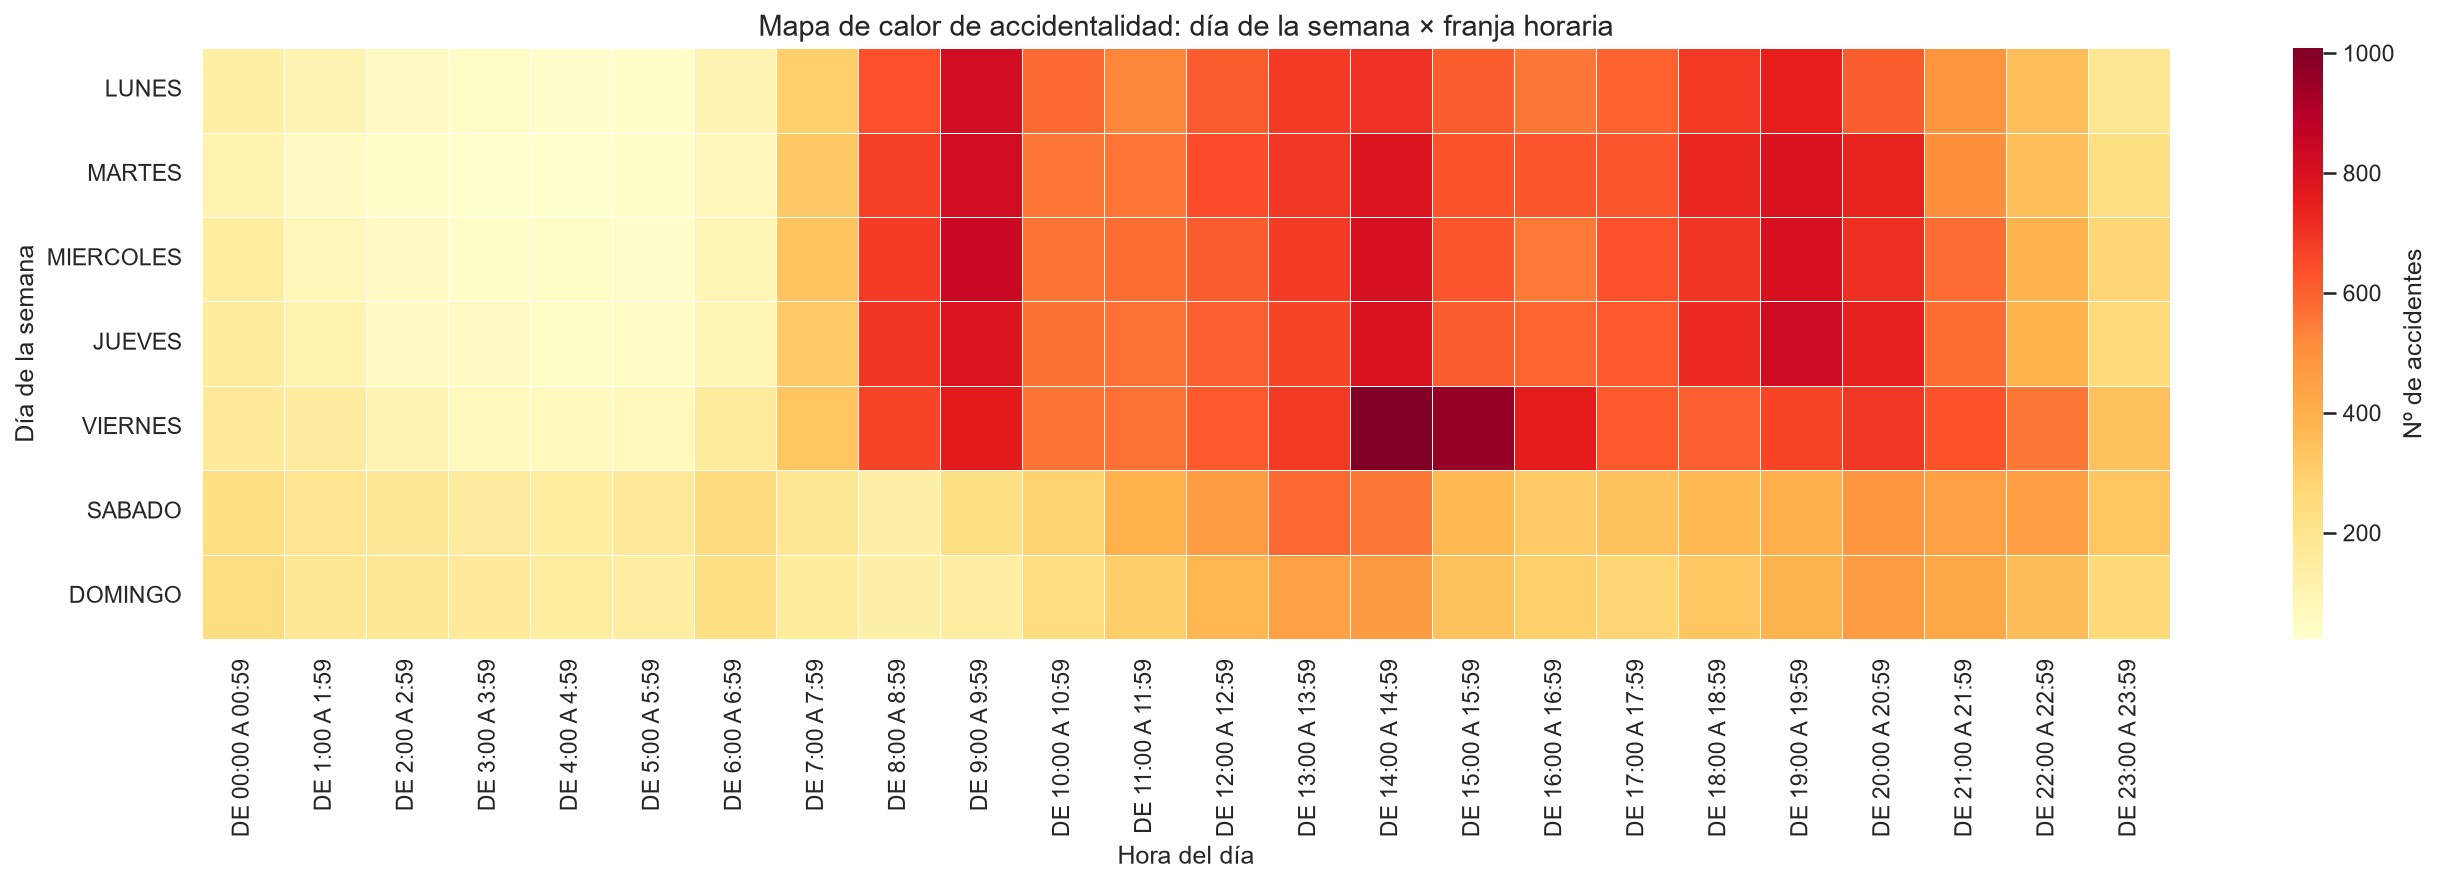
\includegraphics[width=0.8\textwidth]{../figures/07d_heatmap_dia_hora.png}
\caption{Mapa de calor de accidentalidad (volumen) por día de la semana y franja horaria, incluido como contraste con la figura~\ref{fig:heatmap_gravedad}.}
\label{fig:heatmap}
\end{figure}

\subsection{Análisis geográfico}

El recuento bruto de accidentes por distrito no es comparable entre sí sin más: Salamanca puede tener más accidentes que Vicálvaro simplemente por tener más habitantes, no por ser más peligroso. Para relativizar por población hacía falta una variable que el dataset de accidentes no trae --- así que se incorporó una fuente externa, la estadística padronal municipal del Ayuntamiento de Madrid, y se calculó la \textbf{población media aritmética de cada distrito a lo largo de todo el periodo de estudio} (2012--2018), en vez de tomar un único año: una cifra puntual podría no ser representativa de todo el periodo que cubren los accidentes, mientras que la media de los 7 años sí lo es.

Como la variable objetivo es la gravedad, la primera pregunta relevante es si la población de un distrito explica su tasa de accidentes graves --- y no la explica en absoluto (figura~\ref{fig:poblacion_gravedad}): $R^2 = 0{,}001$ ($p = 0{,}88$, no significativo). Es la confirmación cuantitativa, con una variable continua en vez de categórica, de lo ya visto con la V de Cramér (Sección~\ref{sec:asociacion}, $V=0{,}018$): el distrito apenas explica la gravedad, sea cual sea la forma de medir la asociación.

\begin{figure}[h]
\centering
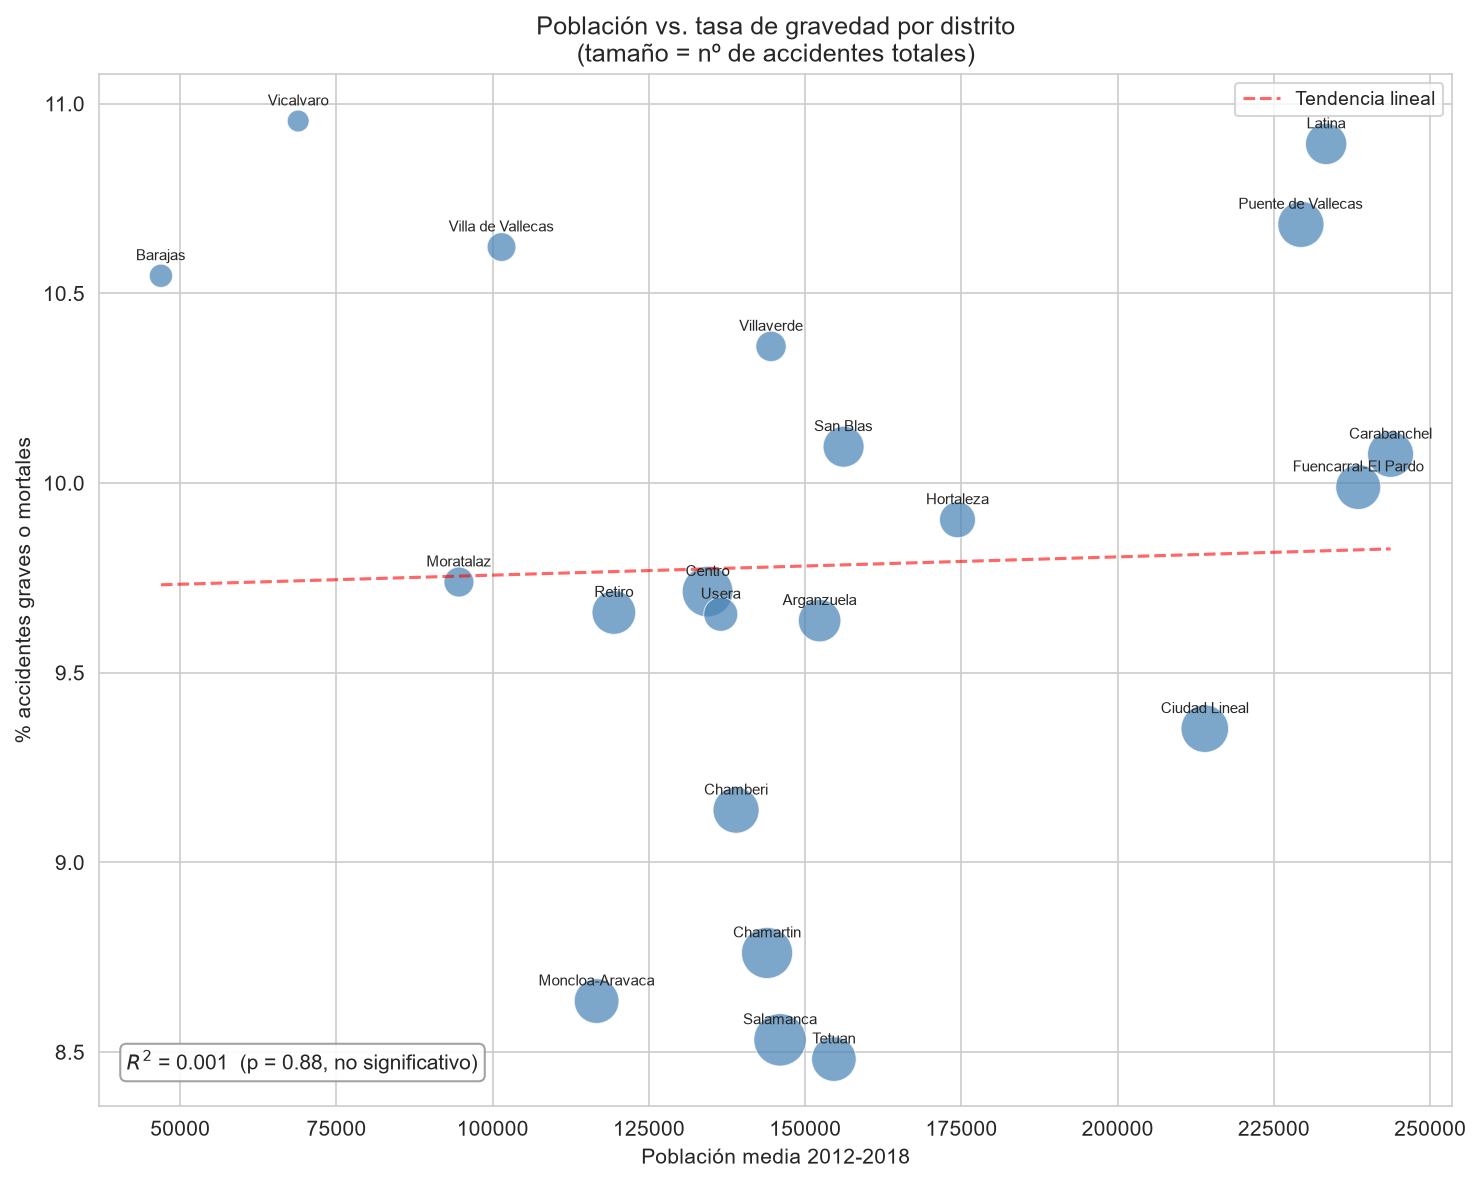
\includegraphics[width=0.8\textwidth]{../figures/08f_scatter_poblacion_gravedad.png}
\caption{Población media frente a tasa de accidentes graves o mortales por distrito (el tamaño de cada punto representa el nº de accidentes totales). La tendencia es prácticamente plana.}
\label{fig:poblacion_gravedad}
\end{figure}

Llevar esa misma tasa a un mapa (figura~\ref{fig:mapa_gravedad}) hace visible el patrón que sí importa, el centro-periferia: los distritos periféricos con vías de alta velocidad --- Vicálvaro (11,0\,\%), Latina (10,9\,\%), Puente de Vallecas (10,7\,\%) y Villa de Vallecas (10,6\,\%)--- concentran la mayor gravedad, mientras que el centro y el noroeste --- Salamanca, Tetuán, Moncloa-Aravaca y Chamartín, todos entre 8,5\,\% y 8,8\,\%--- quedan claramente por debajo de la media. Ni el volumen de población ni el de tráfico explican este patrón: apunta más bien al tipo de vía (carreteras de alta velocidad en la periferia frente a tráfico urbano lento en el centro).

\begin{figure}[htbp]
\centering
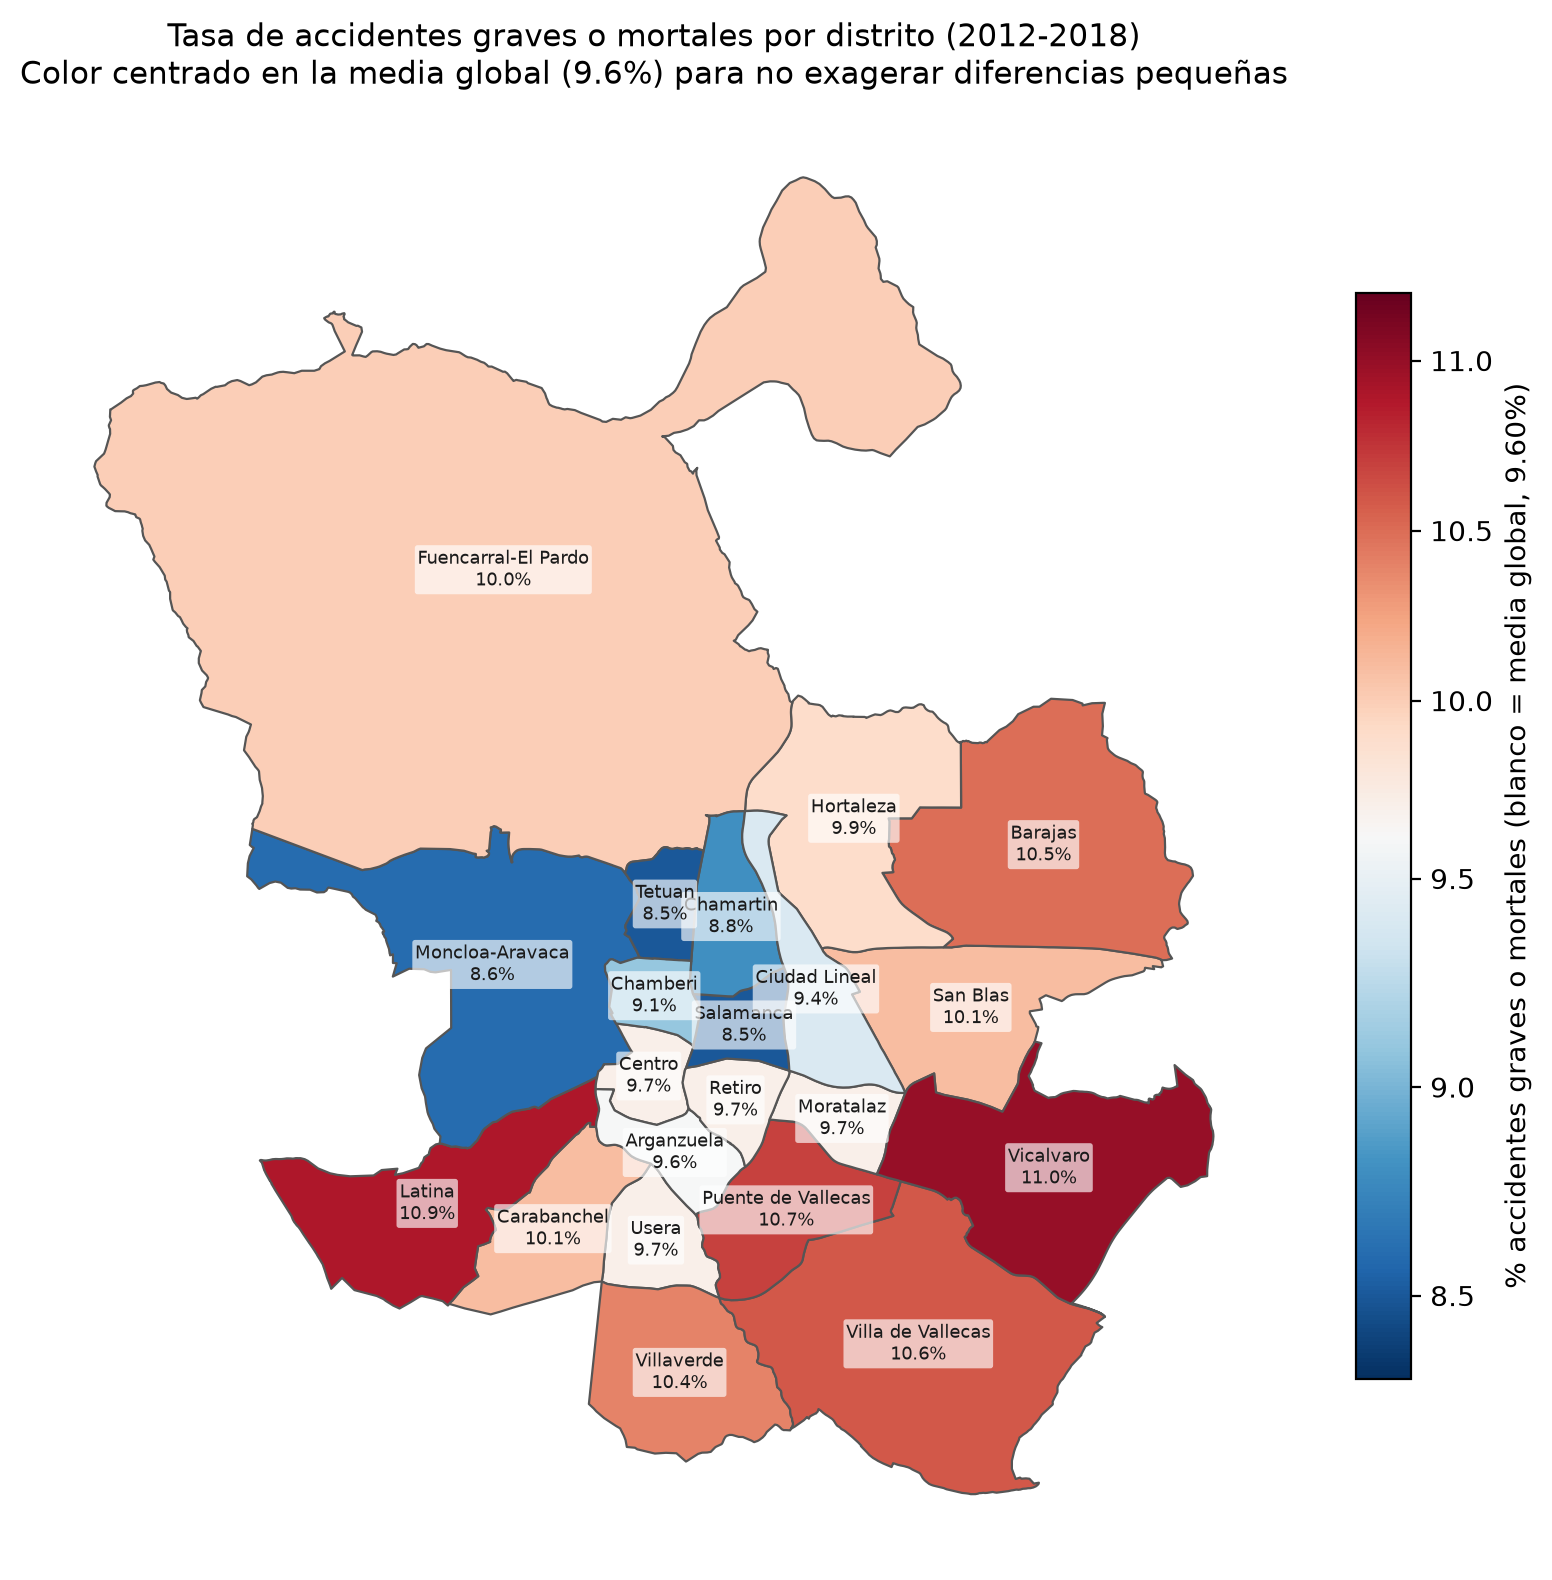
\includegraphics[width=0.75\textwidth]{../figures/08e_mapa_gravedad_distritos.png}
\caption{Mapa de la tasa de accidentes graves o mortales por distrito (2012--2018). Escala de color divergente centrada en la media global (9,60\,\%, en blanco) en vez de en el mínimo y máximo de los 21 distritos, para no exagerar visualmente diferencias de un punto porcentual o menos --- coherente con la escasa asociación ya vista (V de Cramér $=0{,}018$). Versión estática, generada con \texttt{geopandas} a partir de las geometrías oficiales de los 21 distritos, del mismo mapa interactivo (\texttt{folium}) disponible en \texttt{figures/08e\_mapa\_gravedad\_distritos.html} (con la escala de color por defecto).}
\label{fig:mapa_gravedad}
\end{figure}

Por volumen, en cambio, la población sí es una buena predictora (figura~\ref{fig:poblacion}): $R^2 = 0{,}295$ ($p=0{,}011$), aunque con desviaciones notables --- Salamanca, Chamartín y Centro lideran la tasa por 100.000 habitantes sin ser los más poblados, lo que apunta al tráfico de paso como factor adicional del volumen. Se incluye como contraste con las figuras anteriores: la población predice razonablemente el \emph{volumen} de accidentes, pero no dice nada sobre su \emph{gravedad}.

\begin{figure}[h]
\centering
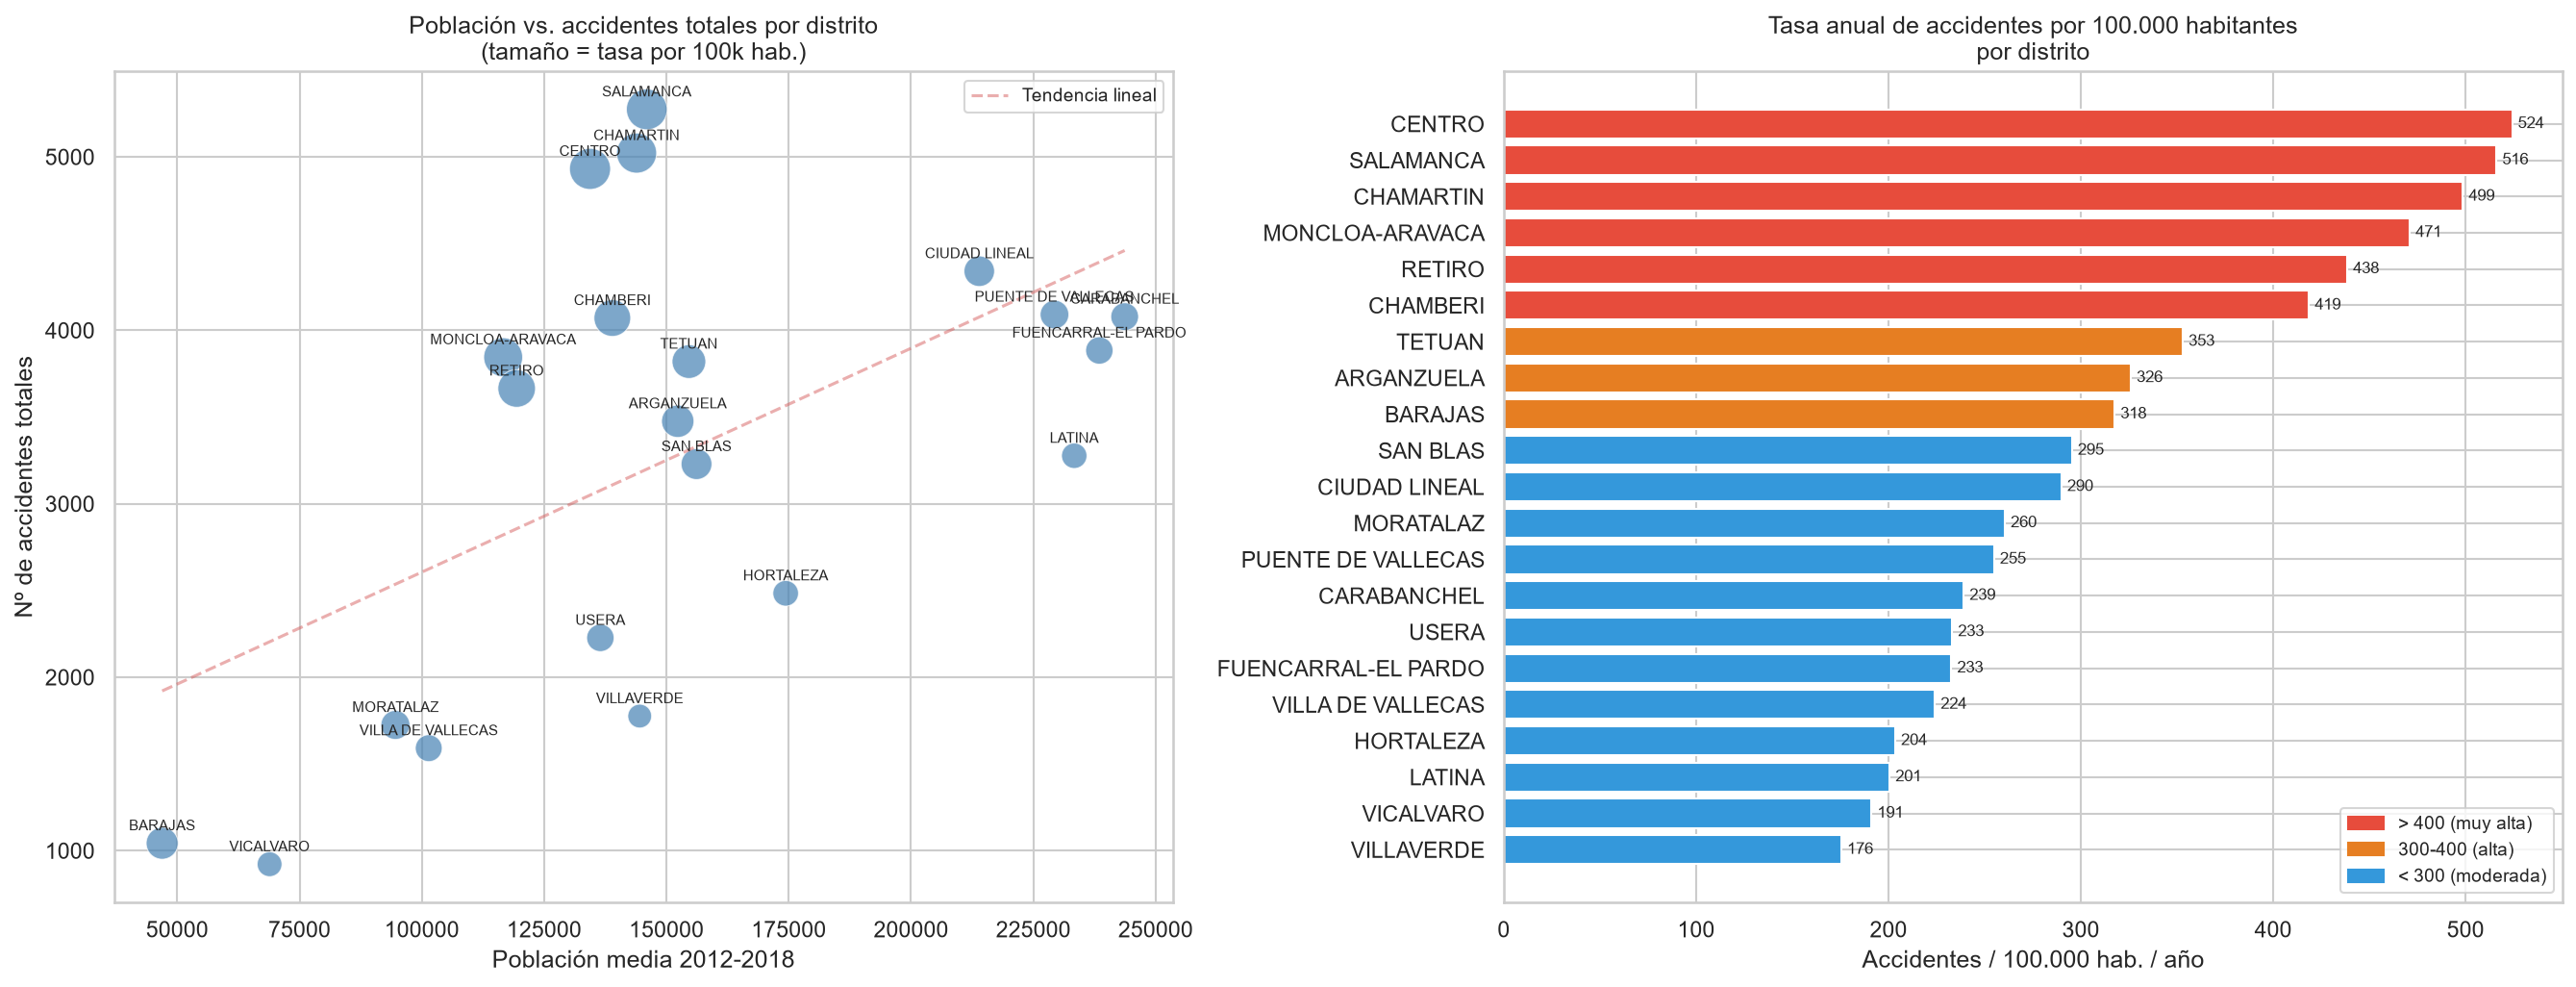
\includegraphics[width=0.8\textwidth]{../figures/08b_scatter_poblacion_accidentes.png}
\caption{Población media frente a accidentes totales por distrito (el tamaño de cada punto representa la tasa de accidentes por 100.000 habitantes), incluida como contraste con la figura~\ref{fig:poblacion_gravedad}.}
\label{fig:poblacion}
\end{figure}

\begin{figure}[htbp]
\centering
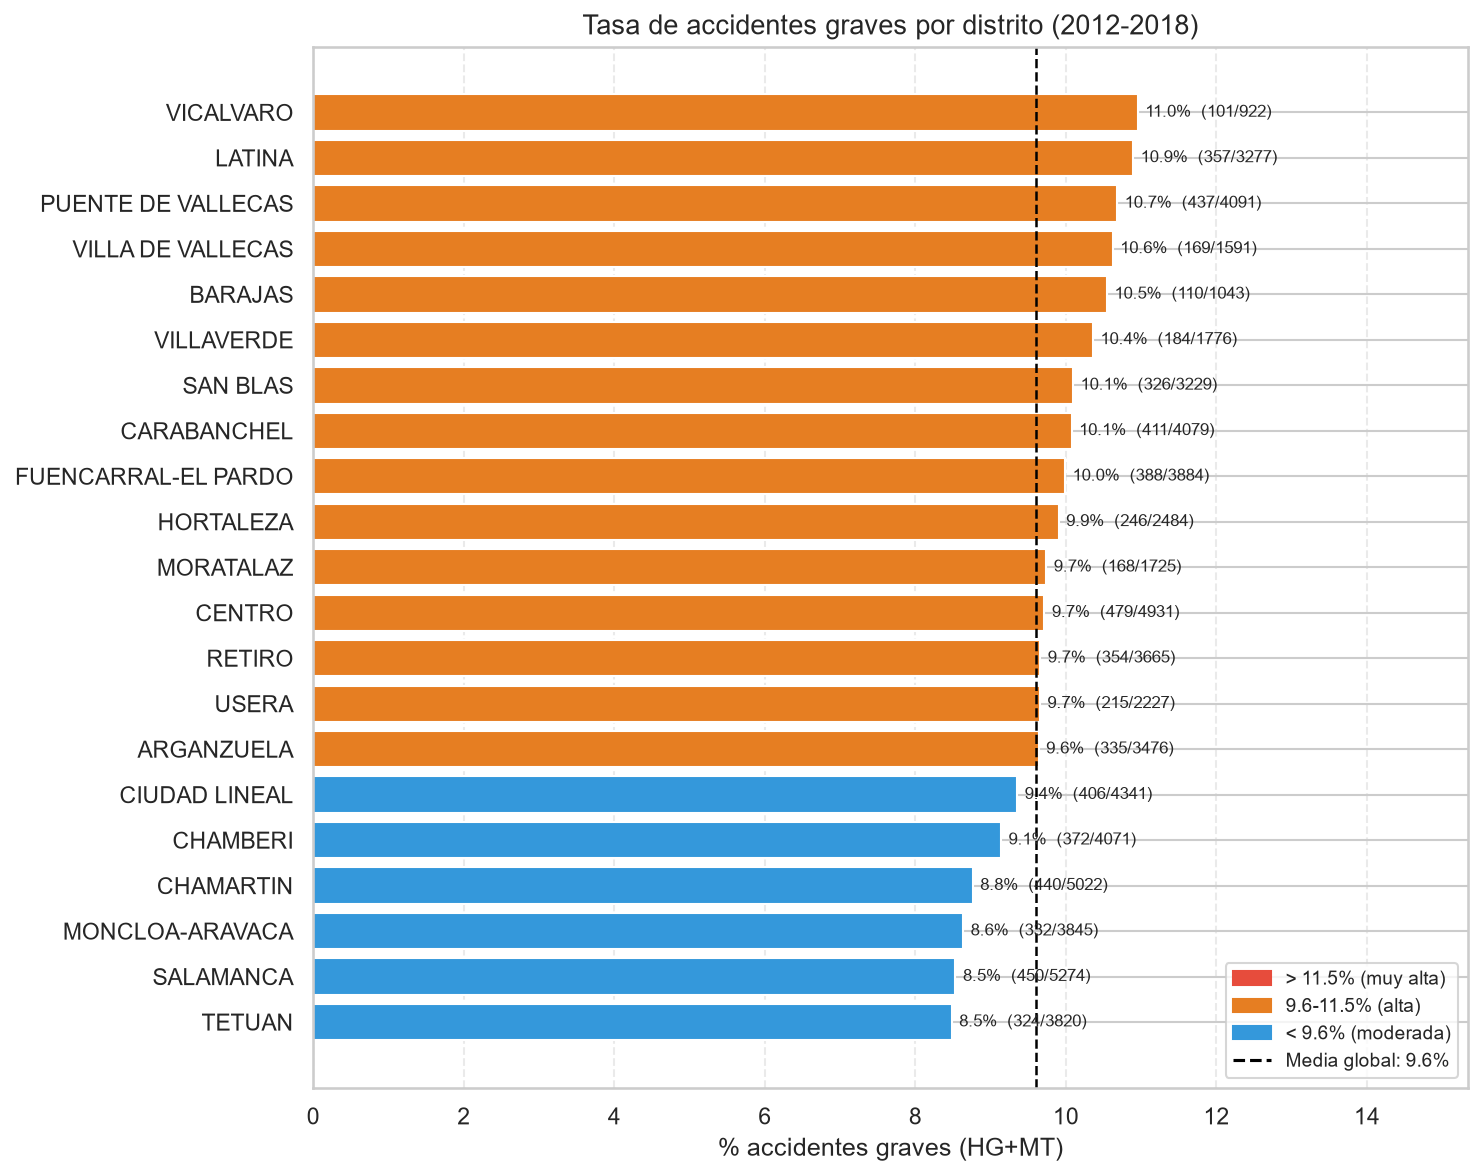
\includegraphics[width=0.62\textwidth]{../figures/08c_tasa_grave_distrito.png}
\caption{Tasa de accidentes graves o mortales por distrito (2012--2018), frente a la media global (9,6\,\%).}
\label{fig:tasa_distrito}
\end{figure}

\subsection{Condiciones del accidente}

\begin{itemize}[nosep]
\item \textbf{Tipo de siniestro:} la colisión doble es la más frecuente (>50\,\%), seguida del atropello y la caída de motocicleta; la caída de bicicleta tiene la mayor proporción de heridos graves.
\item \textbf{Meteorología:} predomina la vía seca (87,2\,\%), con la mayor tasa de gravedad entre las condiciones con muestra suficiente (4,43\,\%). De forma contraintuitiva, la lluvia se asocia con \emph{menor} gravedad (3,43\,\%, diferencia significativa) --- coherente con la hipótesis de compensación de riesgo: los conductores extreman la precaución en condiciones adversas.
\item \textbf{Estado del firme:} la grava suelta (10,35\,\%) y el aceite (4,64\,\%) tienen la mayor tasa de gravedad, aunque son poco frecuentes; la gran mayoría de accidentes ocurre en firme seco y limpio.
\end{itemize}

\subsection{Valores atípicos: número de víctimas}

La única variable numérica del dataset, \texttt{Nº VICTIMAS}, presenta una distribución muy asimétrica a la derecha: el 71,9\,\% de los accidentes tiene una sola víctima, con una cola larga de casos con varias. Antes de decidir cómo tratarla se comprobó qué criterio de valores atípicos es aplicable, en vez de asumir el habitual por defecto.

El criterio del rango intercuartílico (IQR) resulta degenerado aquí: como Q1 = Q3 = 1, el IQR vale 0, y aplicarlo marcaría cualquier accidente con dos o más víctimas como atípico --- un 19\,\% del dataset, un falso positivo masivo. La alternativa de la regla $3\sigma$ tampoco es apropiada: el test de Lilliefors rechaza la normalidad de la variable (asimetría 4,68, curtosis 44), supuesto del que depende esa regla. Se adopta en su lugar un criterio de \textbf{percentiles empíricos}, que no asume ninguna forma de distribución: al percentil 95 se consideran atípicos los accidentes con más de 3 víctimas (2,00\,\%); al 99, más de 4 (0,80\,\%).

\begin{figure}[h]
\centering
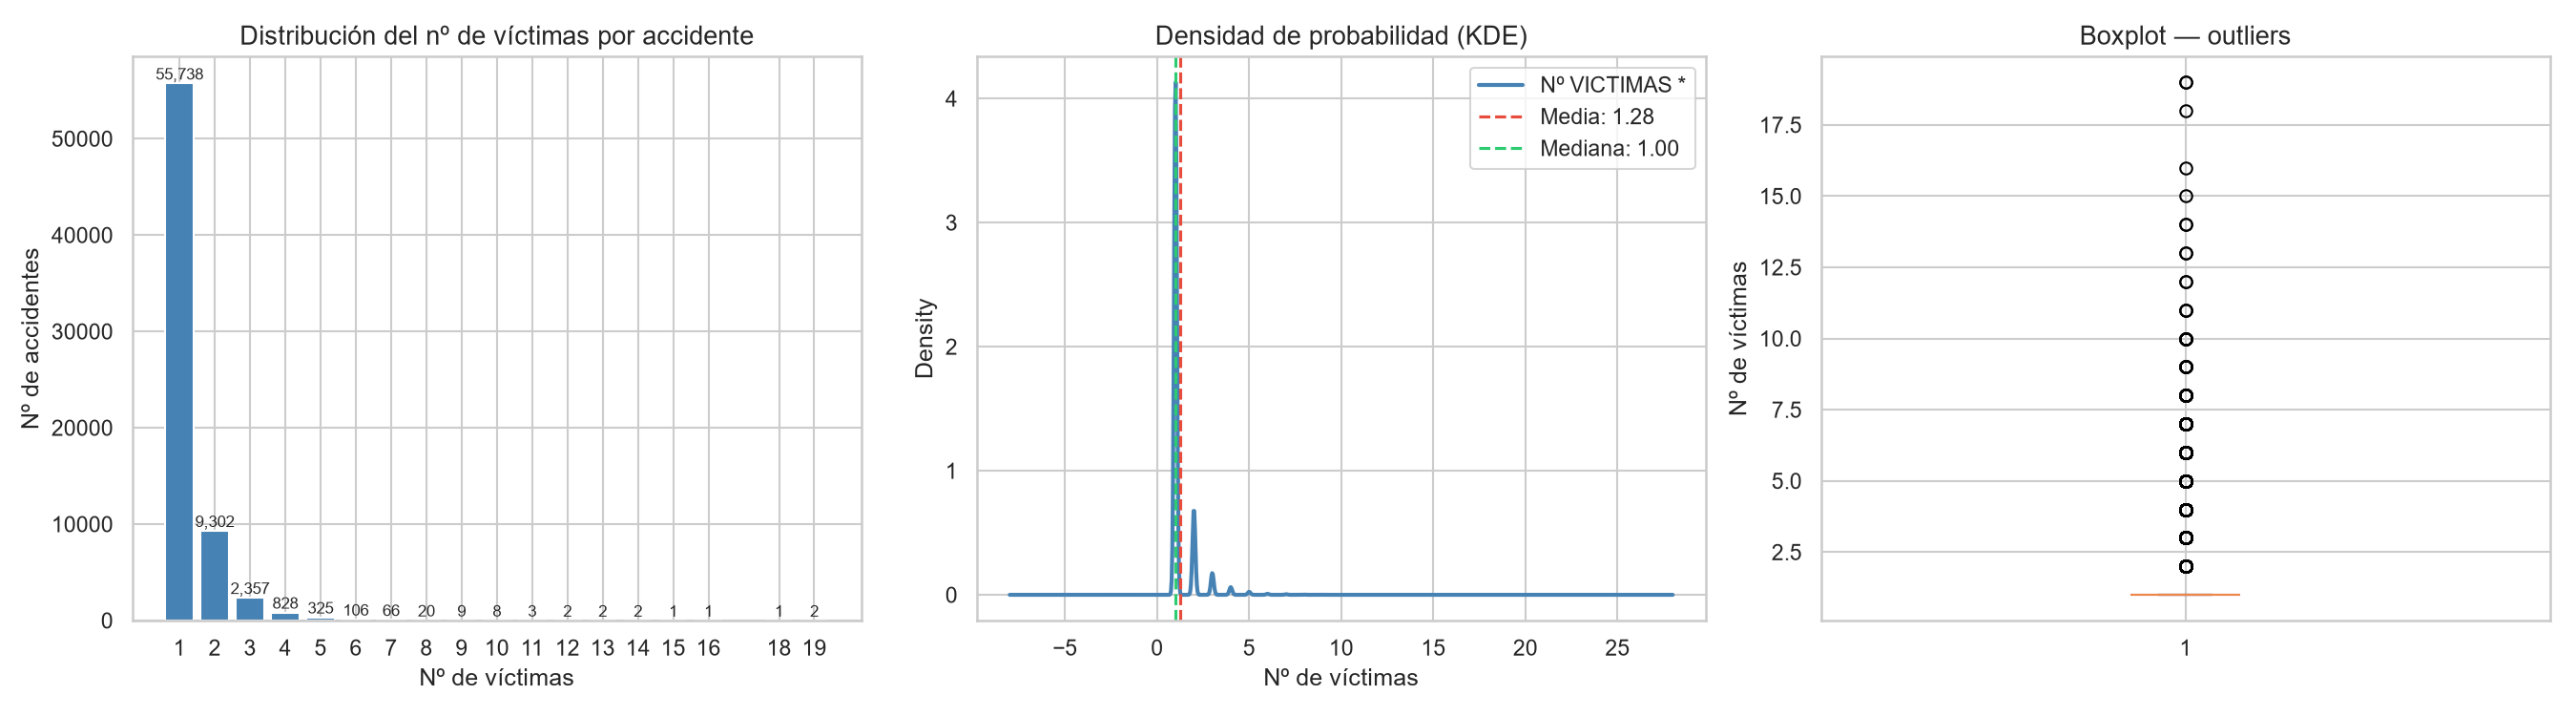
\includegraphics[width=0.8\textwidth]{../figures/06a_distribucion_victimas.png}
\caption{Distribución del número de víctimas por accidente (boxplot con bigotes al percentil 99, ya que el criterio IQR por defecto es degenerado para esta variable).}
\label{fig:victimas}
\end{figure}

Identificados los valores atípicos, se decide \textbf{no eliminarlos}: no son errores de captura, sino accidentes reales con varios implicados, y \texttt{Nº VICTIMAS} queda de todos modos excluida como variable predictora en la fase de modelización, al ser una consecuencia del propio accidente que solo se conoce después (el mismo criterio de fuga de información temporal aplicado al resto de variables posteriores al aviso). Sí se conserva una versión transformada logarítmicamente para atenuar su asimetría, usada únicamente en la matriz de referencia del modelo explicativo (Sección~3.4).

Aun excluidos como predictor, estos valores atípicos importan para entender la gravedad (figura~\ref{fig:victimas_gravedad}): el \% de accidentes graves se mantiene estable en torno al 9--10\,\% hasta 6 víctimas, pero se dispara al 23\,\% en los accidentes con 7 o más --- el grupo más extremo (percentil 99) es también, con diferencia, el más grave, aunque su tamaño de muestra (117 accidentes) exige cautela.

\begin{figure}[h]
\centering
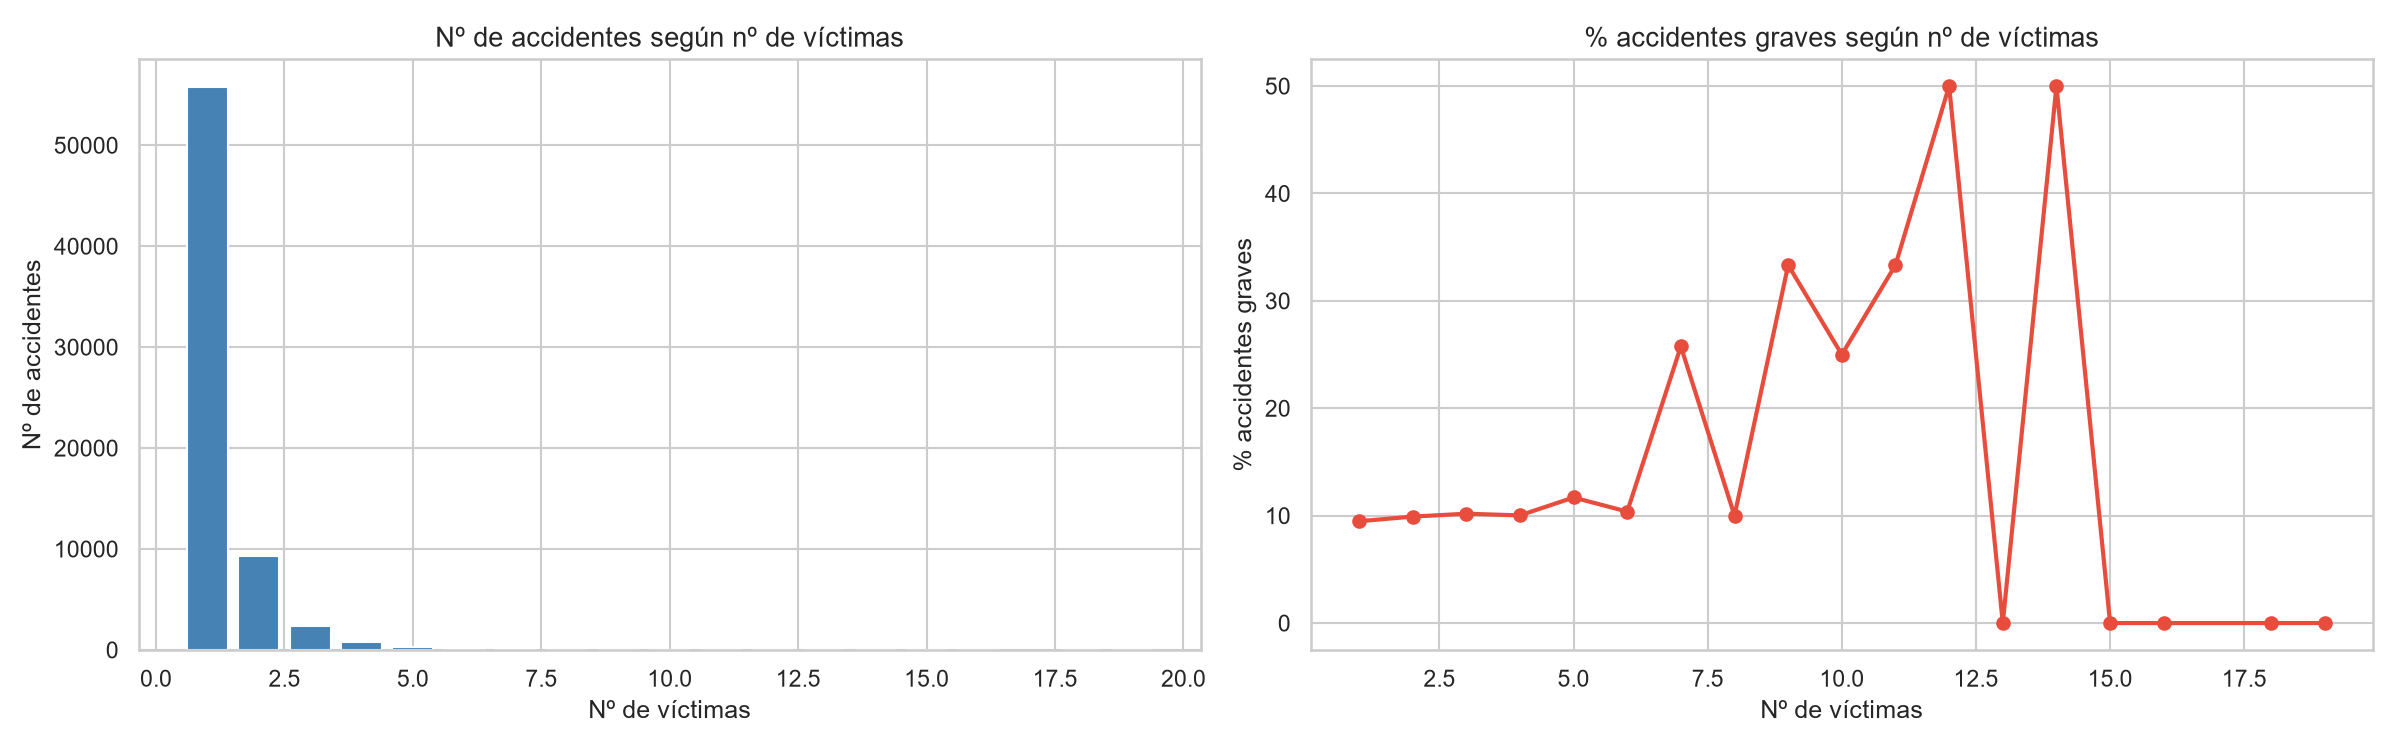
\includegraphics[width=0.95\textwidth]{../figures/06b_victimas_vs_gravedad.png}
\caption{Izquierda: número de accidentes según nº de víctimas. Derecha: \% de accidentes graves según nº de víctimas, con el tamaño de muestra de cada grupo.}
\label{fig:victimas_gravedad}
\end{figure}

\subsection{Asociación estadística con la gravedad}
\label{sec:asociacion}

Para identificar qué variables se relacionan más con la gravedad se calculó la \textbf{V de Cramér} de cada variable categórica frente al objetivo --- de 0 (nula) a 1 (perfecta) --- junto con un \textbf{test chi-cuadrado} que confirma si la relación es significativa o podría deberse al azar (función y corrección de Bonferroni en el Anexo~\ref{app:cramer}). Un punto metodológico central: las variables de persona (tipo de persona, sexo, edad, vehículo) varían entre los implicados de un mismo accidente, pero las de accidente (distrito, franja horaria, tipo de siniestro...) son idénticas para todos ellos. Testear estas últimas a nivel persona repetiría cada accidente una vez por implicado, inflando el tamaño muestral y sobrestimando su relevancia (pseudo-replicación). Por eso cada variable se testeó en su nivel real de variación, y el umbral de significancia se corrigió por el número de comparaciones (Bonferroni, $\alpha = 0{,}0024$ para 21 variables).

\begin{figure}[htbp]
\centering
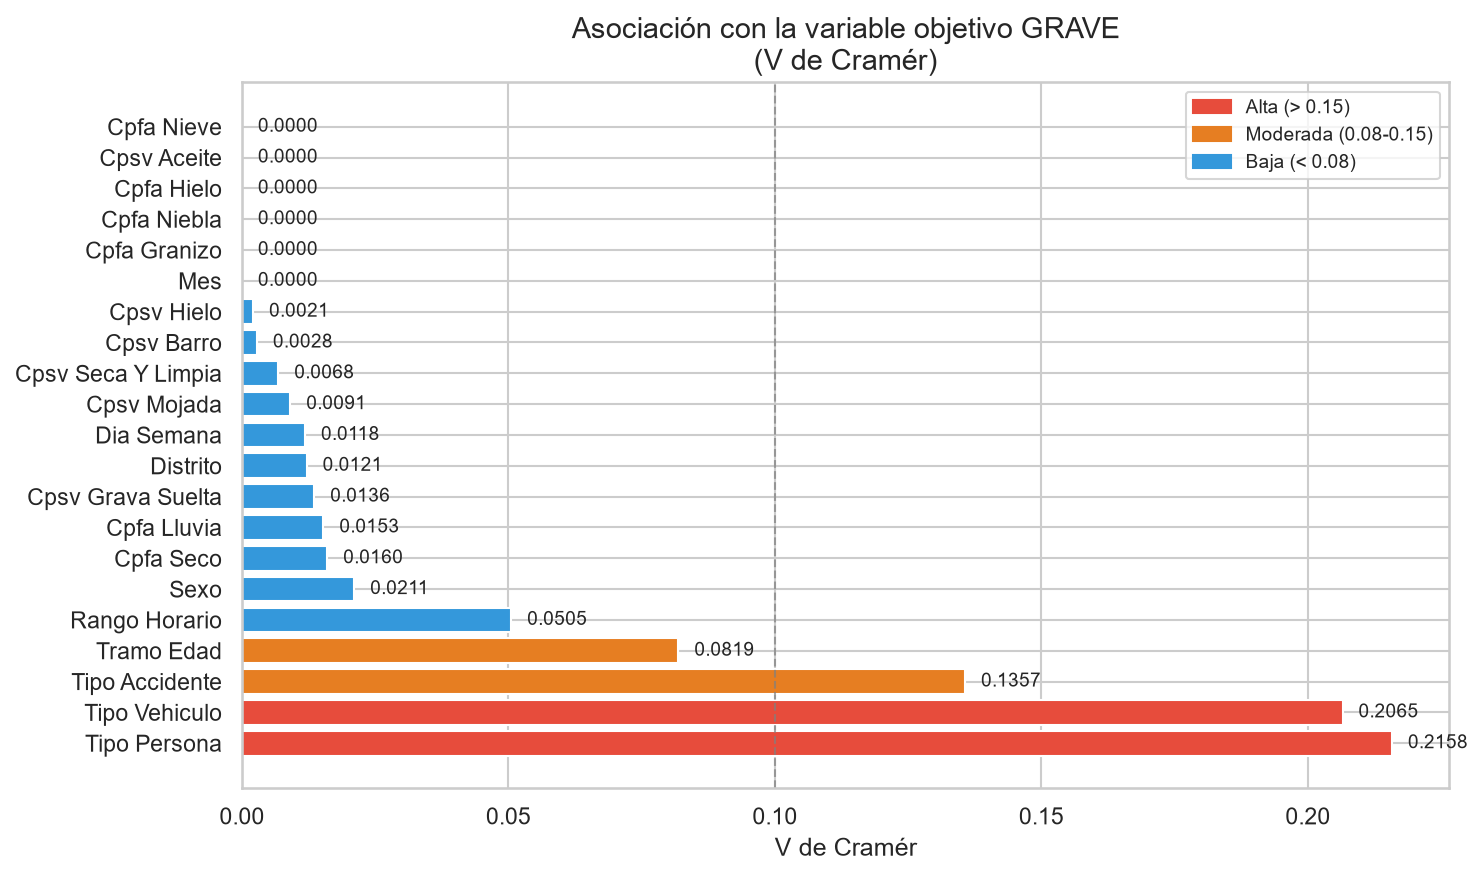
\includegraphics[width=0.8\textwidth]{../figures/10a_cramer_v_asociacion.png}
\caption{Asociación de todas las variables categóricas con GRAVE (V de Cramér). Las condiciones atmosféricas y de firme más raras (granizo, hielo, nieve...) quedan cerca de cero, coherente con su tamaño muestral insuficiente.}
\label{fig:cramer}
\end{figure}

\begin{table}[h]
\centering
\small
\begin{tabular}{lccl}
\toprule
\textbf{Variable} & \textbf{V de Cramér} & \textbf{Nivel} & \textbf{Observación} \\
\midrule
Tipo de persona & 0,216 & Persona & Los peatones concentran la mayor gravedad \\
Tipo de vehículo & 0,207 & Persona & Motos y bicicletas, mayor gravedad \\
Tipo de accidente & 0,172 & Accidente & Alta variabilidad según el tipo \\
Tramo de edad & 0,082 & Persona & Mayores de 65 y menores de 18, más vulnerables \\
Franja horaria & 0,062 & Accidente & Mayor gravedad en horario nocturno \\
Día de la semana & 0,022 & Accidente & Diferencias laborables/fin de semana \\
Sexo & 0,021 & Persona & Gravedad relativa similar entre sexos \\
Distrito & 0,018 & Accidente & Explica el volumen, apenas la gravedad \\
\bottomrule
\end{tabular}
\caption{Asociación de las principales variables categóricas con la gravedad (V de Cramér, medidas en su nivel real de variación).}
\label{tab:cramer}
\end{table}

La tabla se puede leer también de forma visual (figura~\ref{fig:distribucion_variables}): al comparar la distribución de grave frente a no grave para tres de estas variables, tipo de accidente muestra proporciones claramente distintas entre clases (coherente con su V alta, 0,172), franja horaria una diferencia más sutil (V moderada, 0,062), y distrito barras casi indistinguibles (V casi nula, 0,018) --- la misma jerarquía que la tabla~\ref{tab:cramer}, pero visible de un vistazo.

\begin{figure}[htbp]
\centering
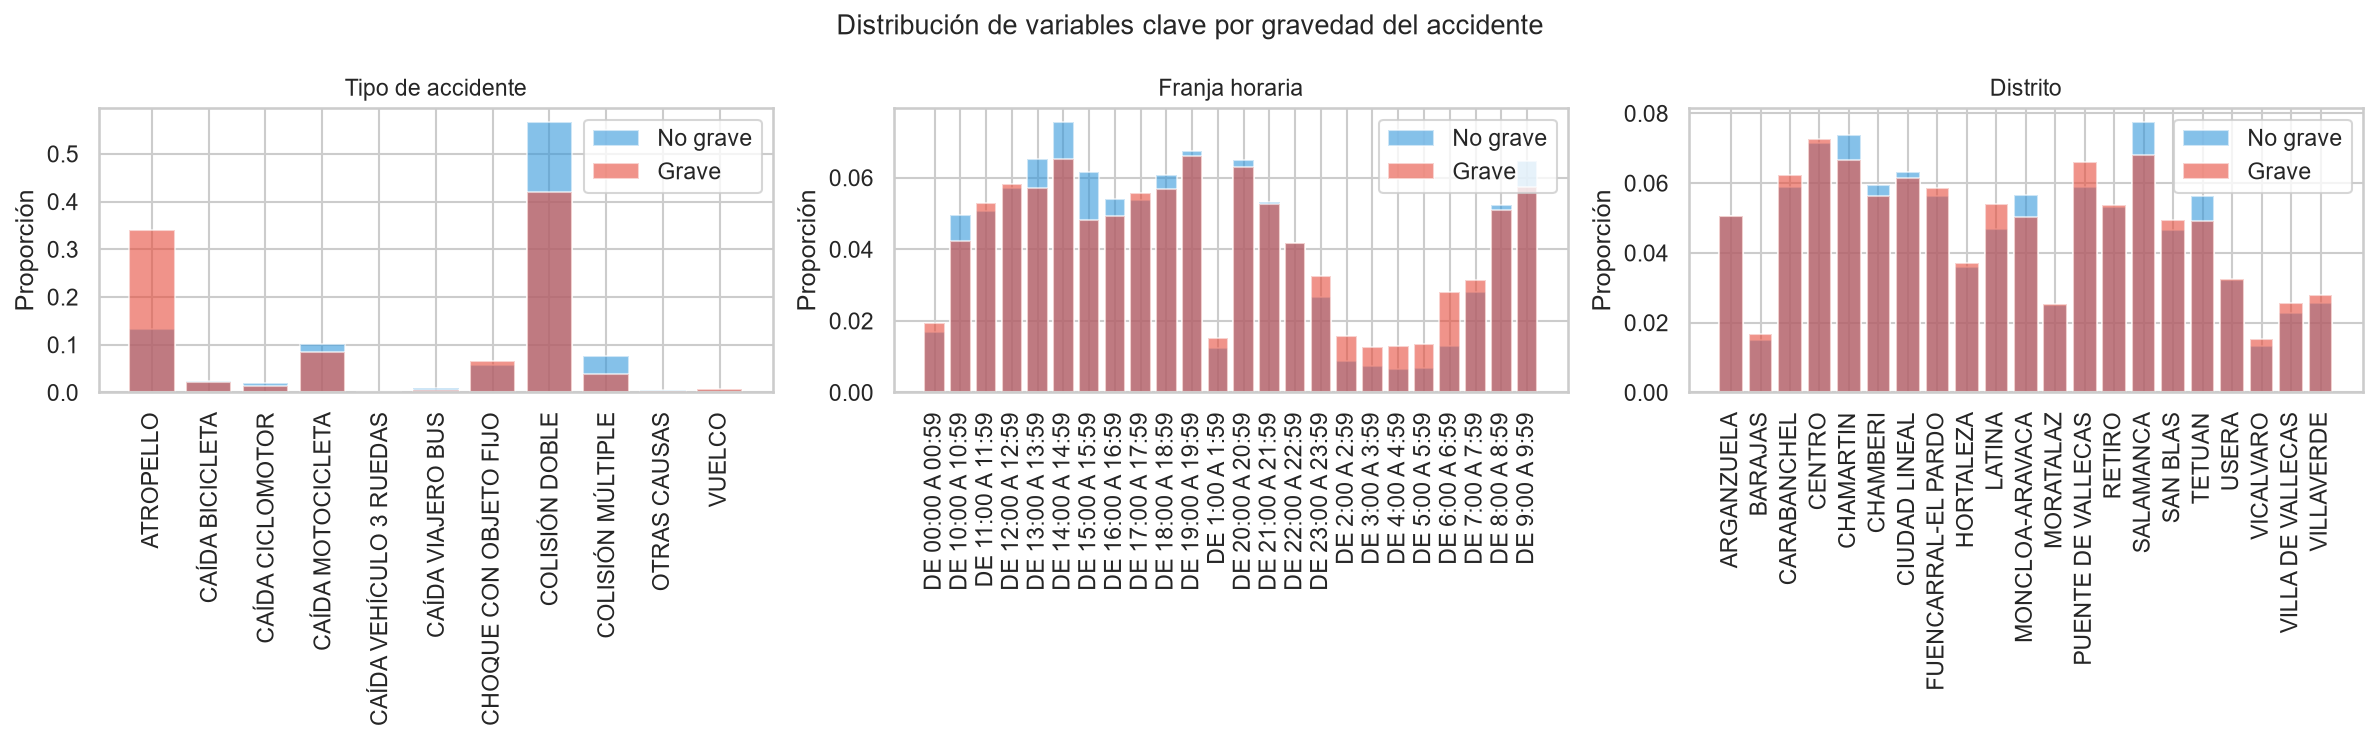
\includegraphics[width=0.95\textwidth]{../figures/05a_desbalanceo_clases.png}
\caption{Distribución de tipo de accidente, franja horaria y distrito, separada por grave/no grave. El grado de solapamiento entre barras anticipa la V de Cramér de cada variable.}
\label{fig:distribucion_variables}
\end{figure}

El chi-cuadrado, ya corregido, confirma como significativas todas las variables de la tabla~\ref{tab:cramer} salvo el mes, más la lluvia y la vía seca. Las condiciones más raras --- granizo, hielo, niebla, nieve, aceite, grava suelta--- quedan cerca de cero en la figura~\ref{fig:cramer}, pero no porque no haya asociación: son tan poco frecuentes (el granizo aparece en solo 9 accidentes de la muestra de test) que ni el chi-cuadrado ni el test exacto de Fisher tienen potencia suficiente para concluir nada. Es una limitación de tamaño muestral, no evidencia de ausencia de asociación --- distinción que se mantiene también en la fase de interpretabilidad.

Como comprobación adicional, se cruzaron pares de variables para detectar efectos condicionados que un análisis univariante no vería: los peatones atropellados presentan la tasa de heridos graves y fallecidos más alta de todas las combinaciones persona-accidente, y las personas mayores de 65 años muestran una gravedad más alta con independencia del tipo de vehículo que conducían o en el que viajaban --- dos patrones que anticipan lo que después confirma, de forma independiente, el análisis de interpretabilidad del modelo explicativo.

% =============================================================================
\section{Preprocesado e ingeniería de variables}
% =============================================================================

\subsection{De nivel persona a nivel accidente}

El dataset crudo está a nivel persona, pero el objeto de estudio es el accidente. La transformación agrega los registros por accidente y separa las variables en dos grupos: las de \emph{accidente} (fecha, distrito, tipo de vía, condiciones), invariantes dentro de un mismo accidente --- comprobado explícitamente columna por columna--- y las de \emph{persona}, que se preservan como indicadores de implicación (¿hubo un peatón, una moto, una persona en edad de riesgo?) por ser las de mayor asociación con la gravedad en el EDA.

La descripción libre de la vía tiene demasiada cardinalidad (>13.000 valores únicos) para usarse como variable categórica. Así que se procesó en dos pasos: 
\begin{enumerate}[nosep]
\item Primero, se detectó el patrón ``vía 1 --- vía 2'' que marca una intersección (46\,\% de los accidentes ocurre en un cruce)
\item Segundo, se clasificó el tipo de vía a partir del texto completo, no solo el primer tramo --- al comprobar que el orden de los dos tramos es alfabético en el 88\,\% de los casos, no indica cuál vía es la relevante (función en el Anexo~\ref{app:preprocesado}).
\end{enumerate}

El efecto de estar en un cruce es débil si se mide de forma aislada (9,45\,\% frente a 9,78\,\%), pero condicionado al tipo de vía y de accidente es mayor y de signo variable: en glorietas eleva la gravedad de 6,8\,\% a 9,7\,\%; en vuelco, +4,2 puntos; en categorías pequeñas como caída de bicicleta, el signo incluso se invierte. La distinta composición de tipos de accidente entre cruces y no-cruces enmascara este efecto real cuando se mide de forma agregada --- por eso se conservó la variable: no por su efecto marginal, sino por su interacción con tipo de vía y de accidente.

El número de víctimas se descartó como predictor: al definirse la gravedad como el máximo entre los implicados, más víctimas implica casi por construcción más probabilidad de que alguna sea grave, y en el momento del aviso no se conoce ese número todavía --- incluirla introduciría fuga de información.

\subsection{Datos ausentes}

Tras agregar a nivel accidente no quedan valores ausentes relevantes en las variables de modelización. Se estableció, de todos modos, una regla explícita para datos nuevos con huecos: las categóricas se imputan con ``Desconocido'' en lugar de eliminar filas, y las numéricas con la mediana del conjunto de entrenamiento, nunca del dataset completo, para no filtrar información hacia el conjunto de prueba.

\subsection{División en conjuntos de entrenamiento y prueba}

Se valoraron dos estrategias: una temporal (entrenamiento 2012--2017, prueba 2018) y una aleatoria estratificada. La temporal es más honesta de cara a un despliegue real --- comprueba si el modelo generaliza a un periodo no visto--- y se documenta como principal; la aleatoria sirve de referencia secundaria. Cualquier estadístico derivado de los datos (medias históricas, categorías de referencia, medianas) se ajusta solo sobre entrenamiento y se aplica después a prueba, replicando lo que ocurriría en producción. El desequilibrio de clases (9,6\,\% graves) se deja sin corregir aquí, como decisión de la fase de modelización.

\subsection{Dos matrices de variables}

Coherente con las dos preguntas de investigación, se construyeron dos matrices de variables a partir del mismo conjunto preprocesado:

\begin{itemize}
\item \textbf{Matriz operativa} (38 variables): únicamente información disponible en el momento del aviso (lugar, momento, condiciones, tipo de vía y de siniestro, más un agregado histórico de gravedad y de composición de vehículos por distrito).
\item \textbf{Matriz de referencia} (42 variables): todo lo anterior más las variables de persona (presencia de peatón, presencia de una persona en edad de riesgo, número de personas implicadas y número de víctimas, transformado logarítmicamente, para atenuar su fuerte asimetría).
\end{itemize}

El distrito ya se representa mediante un agregado histórico, así que no se le aplica además un \emph{one-hot} redundante. Ese agregado se calcula con un suavizado tipo \textbf{Bayes empírico}: la tasa de un distrito con pocos accidentes se combina con la tasa global, ponderada por tamaño de muestra, para que una tasa extrema por puro azar no distorsione el modelo (\emph{target encoding}). En entrenamiento se calcula además fuera de muestra, para que ninguna fila contribuya a su propio valor; en prueba se aplica el mapeo ya aprendido (código en el Anexo~\ref{app:encoding}).

Las \textbf{variables cíclicas} (hora, mes) se codificaron en seno/coseno, para que el modelo no interprete la medianoche y las once de la noche como opuestos. Tipo de vía y tipo de accidente se codificaron en \emph{one-hot} con la categoría más frecuente (calle, colisión doble) como referencia. Antes de ese \emph{one-hot}, las categorías de tipo de accidente con menos de 30 accidentes en entrenamiento se fusionan con ``otras causas'' --- en la práctica, solo afecta a ``caída de vehículo de 3 ruedas'' (6 accidentes en todo el histórico 2012--2018) --- para no crear una columna casi vacía, más inestable de un fold a otro que informativa; el umbral se aprende sobre entrenamiento y se aplica igual sobre prueba y sobre cualquier accidente nuevo.

Las doce columnas de meteorología y firme resultaron ser dos variables categóricas ya codificadas en \emph{one-hot} encubierto (en el 99,9\,\% de los casos, solo una de las seis meteorológicas vale uno): usarlas todas introduciría la trampa clásica de la variable ficticia (colinealidad de $-0{,}98$ entre las dos más frecuentes), así que se eliminó la categoría de referencia de cada grupo (vía seca, firme seco y limpio).

\subsection{Revisión final de colinealidad}

La colinealidad se revisó en dos pasos:
\begin{enumerate}[nosep]
\item Primero, un cribado por pares sobre las 38 variables operativas: solo tres pares superan 0,6, todos con explicación sustantiva --- lluvia y firme mojado (0,89), y la tasa histórica de gravedad del distrito con sus agregados de peatones y motos (0,61 y 0,67, esperable al venir del mismo distrito).
\item  Segundo, el factor de \textbf{inflación de la varianza} (VIF, que mide cuánto predicen todas las demás variables combinadas, no solo una a una): ninguna variable supera 10 (el umbral habitual), y las correlaciones más altas quedan en torno a 5,2, una correlación moderada por pares no implica necesariamente un problema de colinealidad global, y viceversa (cálculo en el Anexo~\ref{app:encoding}).
\end{enumerate}


% =============================================================================
\section{Modelización}
% =============================================================================

\subsection{Algoritmos considerados}

Se entrenaron y compararon cuatro modelos: regresión logística (con ponderación de clases), \emph{Random Forest}, \emph{Gradient Boosting} (variante de histograma) y XGBoost, tres familias de complejidad distinta (lineal, \emph{bagging}, \emph{boosting}), para comparar no solo el rendimiento sino también su comportamiento frente al sobreajuste. Se descartaron SVM y k-neighbors, ya que con más de 55.000 filas, decenas de columnas dispersas y desequilibrio de clases, su coste computacional y peor encaje con este tipo de variables los hace poco prácticos frente a árboles y \emph{boosting}, que además no requieren escalado.

Aunque la variable objetivo es binaria (grave/no grave), ninguno de los cuatro algoritmos predice directamente esa etiqueta: todos estiman una \textbf{probabilidad continua} entre 0 y 1, y la etiqueta se obtiene solo al final, aplicando un umbral (por defecto, 0,5). Todas las métricas de este trabajo --- el área bajo la curva ROC, el área bajo la curva precisión-recall, el \emph{score} de Brier (que mide cuánto se alejan, en promedio, las probabilidades predichas de lo que realmente ocurrió), los propios valores SHAP--- se calculan sobre esa probabilidad continua, no sobre la etiqueta ya umbralizada; es también esa misma probabilidad, sin convertir a una decisión binaria, la que se muestra como resultado en la aplicación de demostración descrita en la Sección~6.

\subsection{Ajuste de hiperparámetros, validación y seguimiento de experimentos}

Cada modelo se ajustó primero sin tunear, para observar su comportamiento predeterminado, y después con una rejilla manual y explícita de combinaciones de hiperparámetros --- en lugar de una búsqueda aleatoria--- para poder inspeccionar directamente el compromiso entre rendimiento y sobreajuste en cada combinación concreta (la función que ejecuta esta rejilla se reproduce en el Anexo~\ref{app:hiperparametros}). La validación durante el ajuste se realizó con una partición temporal dentro del propio conjunto de entrenamiento, consistente con la naturaleza temporal del problema, y el sobreajuste se midió siempre como la diferencia entre el área bajo la curva ROC en entrenamiento y en esa validación cruzada --- nunca contra el conjunto de prueba, que solo se evalúa una única vez, al final, con la configuración ya elegida, para no introducir una fuga de información hacia la evaluación final.

Los cinco grids de esta fase se registraron en Weights \& Biases, para comparar todas las combinaciones en un panel interactivo. Este seguimiento cubre \textbf{únicamente el modelo operativo} (Pregunta 1): el modelo explicativo (Sección~4.5) no pasa por ningún grid, ya que usa la configuración por defecto de cada algoritmo. Figura~\ref{fig:wandb} muestra el panel de XGBoost --- el algoritmo elegido--- coloreado por área bajo la curva ROC de validación cruzada.

\begin{figure}[h]
\centering
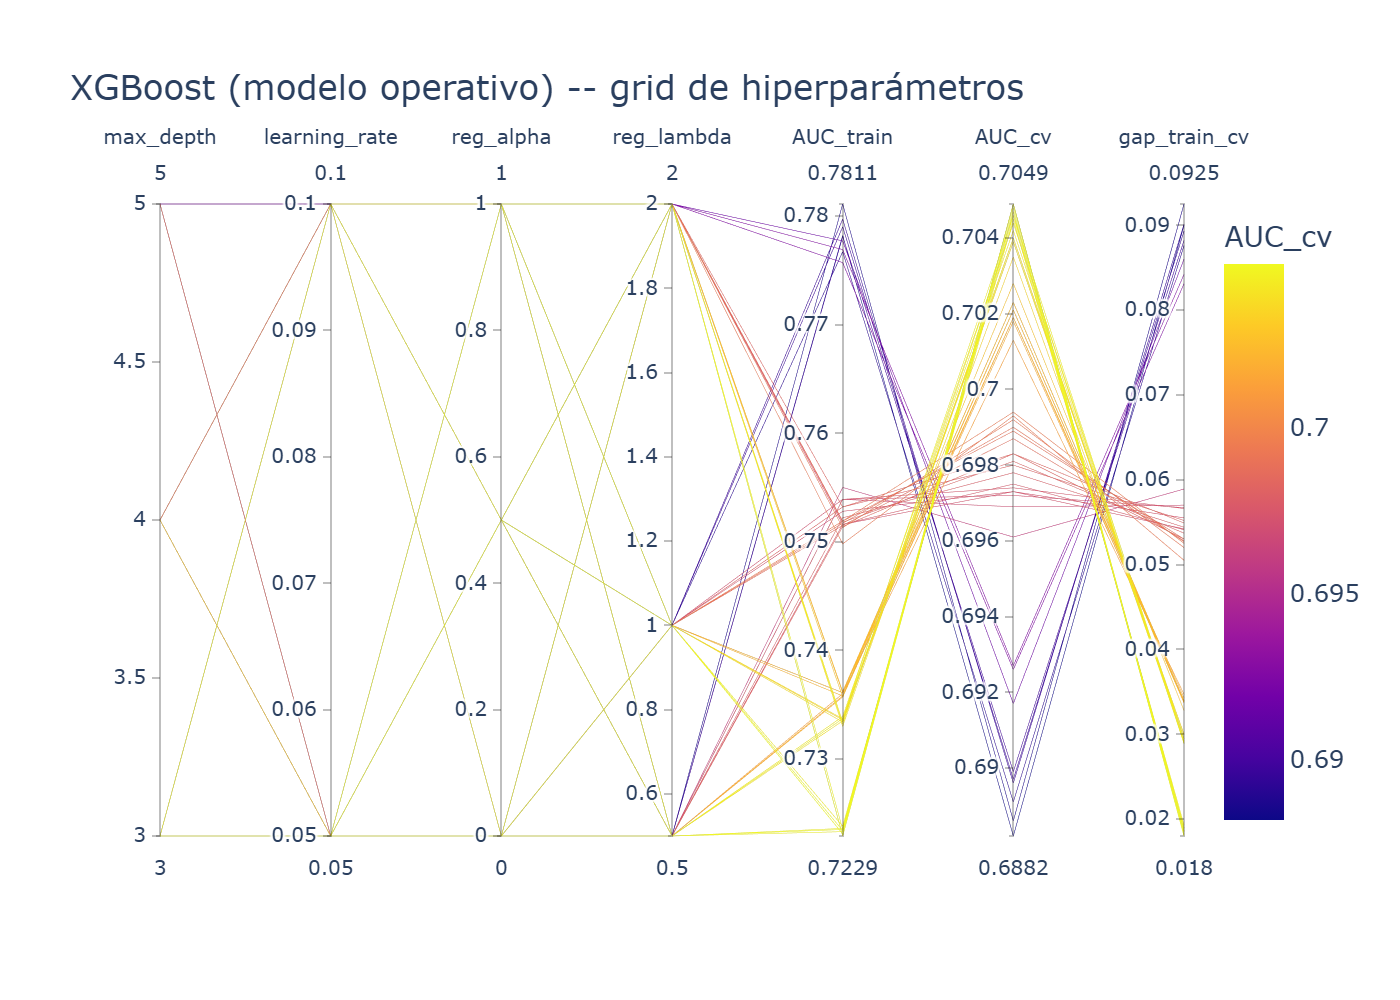
\includegraphics[width=0.85\textwidth]{../figures/04_wandb_xgb.png}
\caption{Panel de coordenadas paralelas del grid de hiperparámetros de XGBoost (modelo operativo, Pregunta 1), registrado en Weights \& Biases.}
\label{fig:wandb}
\end{figure}

Por modelo, lo más relevante del ajuste (fortalezas y debilidades completas en la tabla~\ref{tab:fortalezas}):

\begin{itemize}[nosep]
\item \textbf{Regresión logística:} apenas varía con la regularización (gap siempre 0,006--0,008); se mantuvo el valor por defecto.
\item \textbf{Random Forest:} sin tunear, sobreajuste severo (patrón clásico de árboles sin límite de profundidad). Una rejilla de estabilidad en tres dimensiones confirmó que la profundidad --- no el tamaño de muestra ni el número de árboles--- es lo que corrige el problema (gap de 0,30--0,34 sin límite, a 0,03--0,09 limitando a 5--10). Configuración final: profundidad 8 (función en el Anexo~\ref{app:validaciones}).
\item \textbf{Gradient Boosting:} controla el sobreajuste por diseño (tasa de aprendizaje baja, nodos limitados) y ya generaliza bien sin tunear; la configuración elegida añade algo más de regularización sin coste real de rendimiento.
\item \textbf{XGBoost:} parada temprana real --- entrena hasta 500 árboles pero conserva solo los que mejoran una partición de validación separada; configuración final, 140 de 150 árboles permitidos.
\end{itemize}

\subsection{Resultados del modelo de triaje operativo}

\begin{table}[h]
\centering
\small
\begin{tabular}{lcccc}
\toprule
\textbf{Modelo} & \textbf{AUC-ROC} & \textbf{AUC-PR} & \textbf{Brier} & \textbf{Gap train-test} \\
\midrule
Regresión logística & 0,699 & 0,158 & 0,222 & 0,009 \\
\emph{Random Forest} & 0,693 & 0,166 & 0,223 & 0,027 \\
\emph{Gradient Boosting} & 0,706 & 0,170 & 0,220 & 0,021 \\
\textbf{XGBoost} & \textbf{0,707} & \textbf{0,174} & \textbf{0,219} & 0,015 \\
\bottomrule
\end{tabular}
\caption{Comparación de los cuatro modelos operativos ya ajustados, evaluados una única vez sobre el conjunto de prueba (2018).}
\label{tab:comparacion_operativo}
\end{table}

Las conclusiones de este trabajo se apoyan principalmente en el área bajo la curva ROC, no en el área bajo la curva precisión-recall, aunque el problema esté desequilibrado (9,6\,\% de accidentes graves): el AUC-ROC se usó de forma consistente durante todo el ajuste de hiperparámetros para medir sobreajuste (Sección~4.2) y para la validación temporal (Sección~4.4), así que es la métrica coherente con las decisiones ya tomadas, y su referencia --- 0,5 equivale siempre a azar, sea cual sea el desequilibrio de clases--- es más directa de comunicar a un lector no técnico que la del AUC-PR, cuyo azar de referencia depende de la prevalencia (aquí, 0,096, no 0,5). Ambas métricas coinciden además en el ranking de los cuatro modelos, lo que refuerza que la elección de XGBoost no depende de cuál de las dos se use. Dicho esto, el AUC-PR no es prescindible: un 0,174 frente a un azar de 0,096 es una mejora relativa de casi el doble, mayor de lo que el AUC-ROC por sí solo sugiere --- señal de que, sobre la clase grave en concreto, el modelo aprovecha más señal útil de la que transmite el 0,707 aislado.

\textbf{XGBoost es el modelo operativo elegido}: mejor área bajo la curva ROC y compromiso train-test moderado, seguido muy de cerca por \emph{Gradient Boosting}. El \emph{Random Forest} queda por debajo de los otros tres (el \emph{bagging} generaliza peor que el \emph{boosting} aquí), y la regresión logística es sorprendentemente competitiva --- señal de que buena parte de la información predictiva es aproximadamente lineal. La tabla~\ref{tab:fortalezas} resume fortalezas y debilidades de cada técnica más allá del ranking, la figura~\ref{fig:roc} sus curvas ROC, y la figura~\ref{fig:roc_traintest} el gap train-test de la tabla~\ref{tab:comparacion_operativo} superpuesto sobre la propia curva: la separación entre la curva de entrenamiento (azul) y la de prueba (naranja) es visiblemente mayor en \emph{Random Forest} que en el resto, coherente con su gap de 0,027.

\begin{table}[h]
\centering
\small
\begin{tabular}{p{2.4cm}p{1.3cm}p{4.6cm}p{4.6cm}}
\toprule
\textbf{Modelo} & \textbf{AUC-ROC} & \textbf{Fortalezas} & \textbf{Debilidades} \\
\midrule
Regresión logística & 0,699 &
Interpretable por diseño (sus coeficientes se leen directamente como razones de probabilidades); apenas sobreajusta (gap 0,009); coste computacional mínimo. &
Solo capta relaciones lineales entre variables; no detecta por sí sola interacciones (p. ej. cruce $\times$ tipo de vía) sin que se incluyan explícitamente. \\
\emph{Random Forest} & 0,693 &
Robusto a valores atípicos; no exige escalado de variables; sirve de referencia adicional de importancia de variables. &
Propenso a un sobreajuste severo si no se limita la profundidad (gap hasta 0,30 sin límite); incluso ya corregido, es el modelo con peor discriminación de los cuatro en este problema. \\
\emph{Gradient Boosting} & 0,706 &
Controla el sobreajuste ``de fábrica'' (tasa de aprendizaje baja, nodos limitados); capta interacciones no lineales sin especificarlas a mano; generaliza bien casi sin tunear. &
Menos interpretable que un modelo lineal; su rendimiento es sensible a la tasa de aprendizaje y a la regularización elegidas. \\
\textbf{XGBoost} & \textbf{0,707} &
Mejor discriminación de los cuatro; parada temprana real (entrena hasta 500 árboles pero solo conserva los que mejoran la validación); mejor compromiso train-test de los tres ensamblados (gap 0,015). &
El más complejo de ajustar (más hiperparámetros); menos transparente que un modelo lineal; depende de una librería externa a scikit-learn. \\
\bottomrule
\end{tabular}
\caption{Precisión, fortalezas y debilidades de cada técnica de modelización empleada, para el modelo de triaje operativo.}
\label{tab:fortalezas}
\end{table}

\begin{figure}[h]
\centering
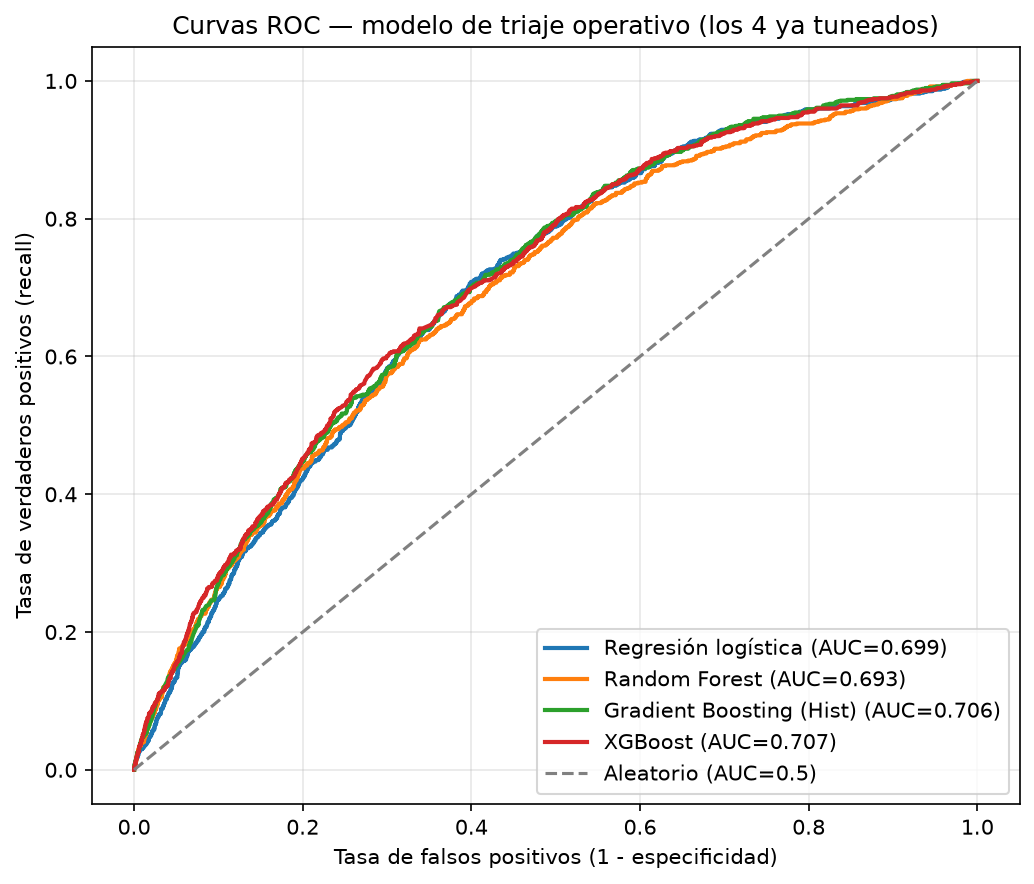
\includegraphics[width=0.6\textwidth]{../figures/12_roc_comparacion_modelos.png}
\caption{Curvas ROC de los cuatro modelos de triaje operativo, evaluadas sobre el conjunto de prueba (2018).}
\label{fig:roc}
\end{figure}

\begin{figure}[h]
\centering
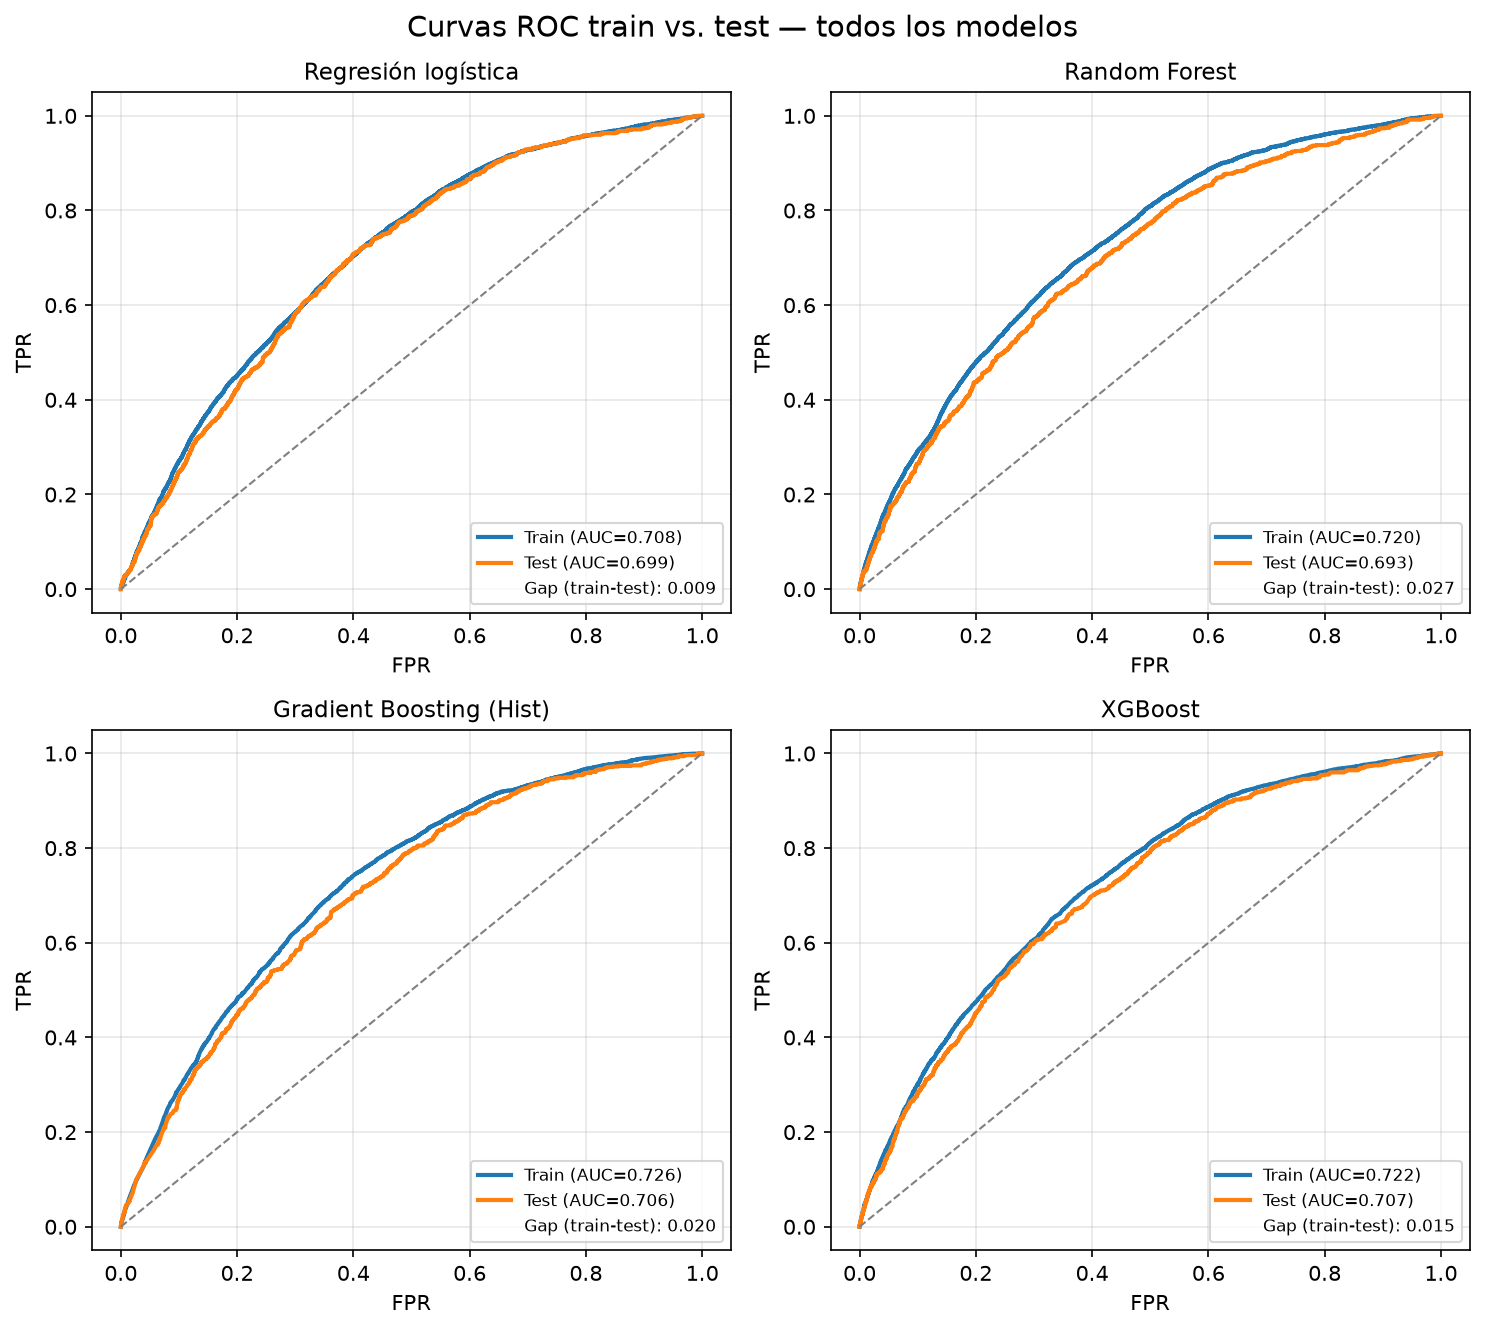
\includegraphics[width=0.85\textwidth]{../figures/13b_roc_train_test_modelos.png}
\caption{Curvas ROC de entrenamiento frente a prueba, por modelo, con el gap train-test correspondiente a la tabla~\ref{tab:comparacion_operativo}.}
\label{fig:roc_traintest}
\end{figure}

\subsection{Calibración y deriva temporal}

Con un umbral de decisión fijo de 0,5, la matriz de confusión de XGBoost sobre el conjunto de prueba (figura~\ref{fig:confusion}) hace tangible el compromiso real que implica ese umbral. De los 874 accidentes realmente graves en 2018, el modelo detecta 621 (sensibilidad o \emph{recall} del 71,1\,\%), pero a costa de 4.100 falsas alarmas sobre los 9.804 accidentes que en realidad no eran graves: de cada accidente marcado como grave, solo el 13,2\,\% (\emph{precisión}) lo es de verdad. Esto no es un fallo del modelo, sino la consecuencia directa de entrenar con ponderación de clases (\texttt{class\_weight='balanced'}, o su equivalente en XGBoost) para que no ignore la clase minoritaria --- un ajuste que desplaza el umbral efectivo de decisión y favorece deliberadamente la sensibilidad sobre la precisión, precisamente el compromiso que interesa en un contexto de triaje, donde el coste de no avisar de un accidente grave (falso negativo) es mayor que el de una alerta de más (falso positivo). Por esta razón las métricas principales de comparación entre modelos son el área bajo la curva ROC y bajo la curva precisión-recall, que no dependen de un umbral concreto; el umbral de 0,5 usado aquí es solo ilustrativo, y en un despliegue real debería ajustarse explícitamente según el coste relativo de cada tipo de error --- y conviene que quien opere la aplicación de triaje (Sección~6.3) conozca esta baja precisión: la mayoría de las alertas de gravedad alta serán, en la práctica, falsas alarmas.

\begin{figure}[htbp]
\centering
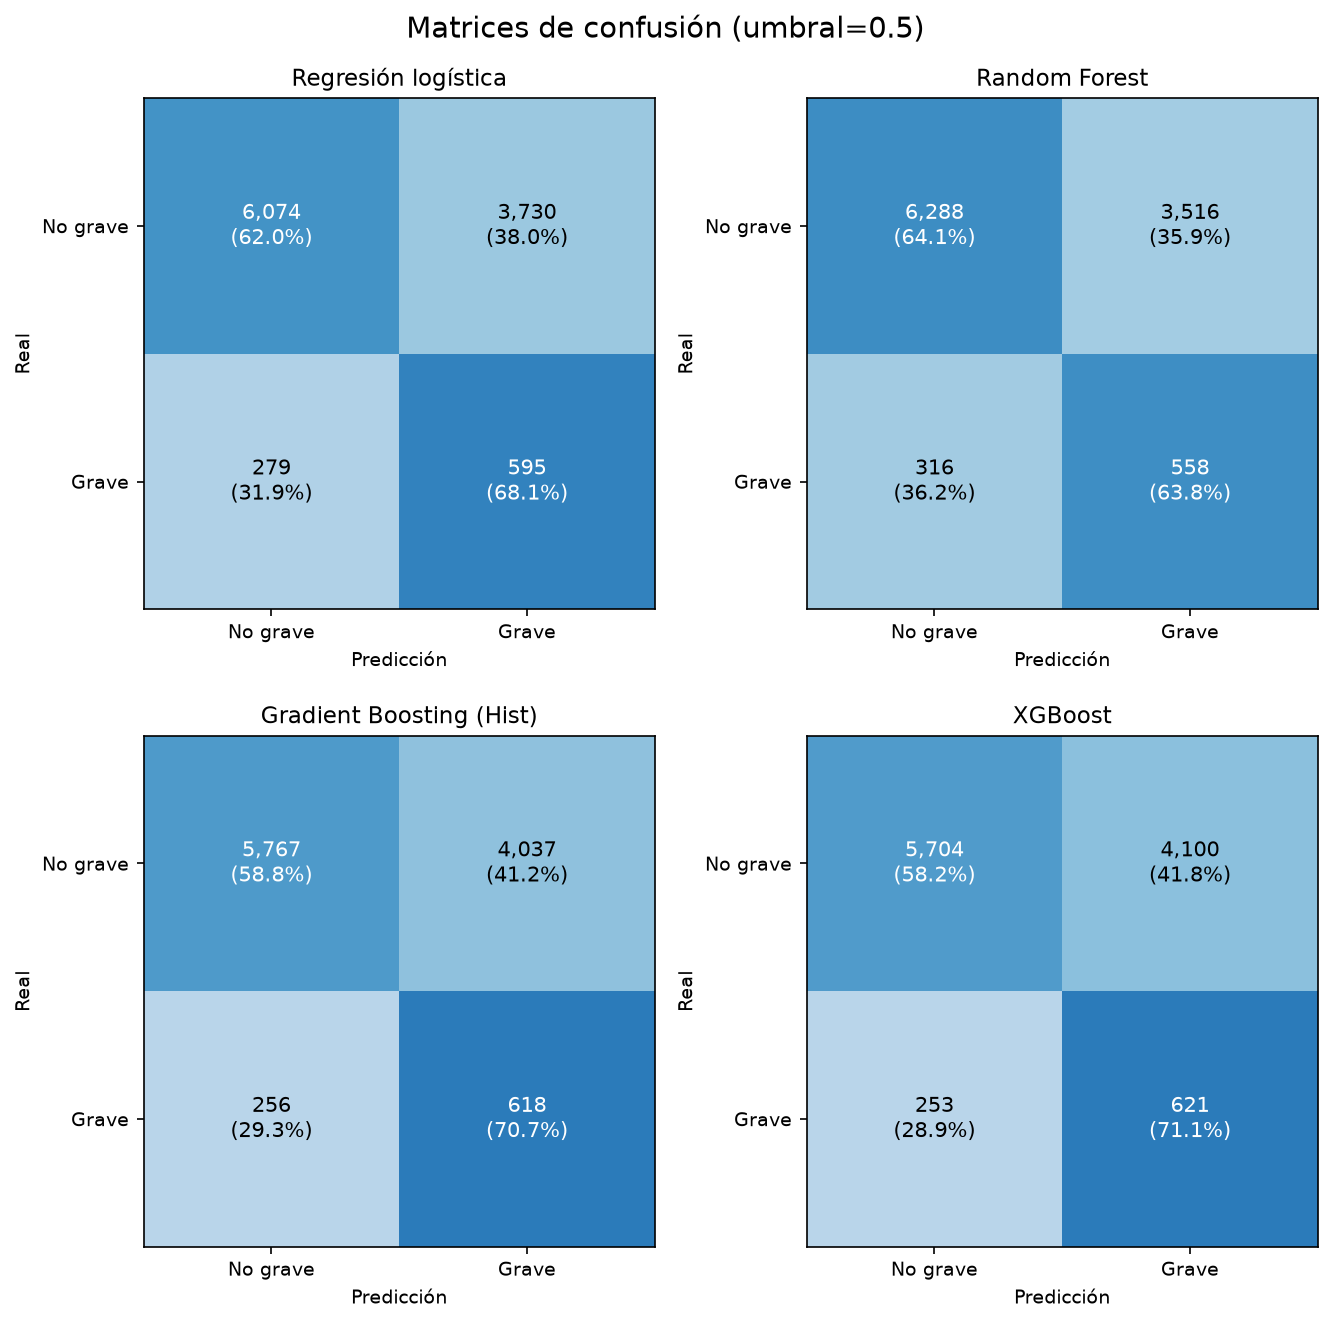
\includegraphics[width=0.85\textwidth]{../figures/16_matrices_confusion_modelos.png}
\caption{Matrices de confusión de los cuatro modelos operativos sobre el conjunto de prueba (2018), umbral de 0,5, normalizadas por fila (porcentaje sobre cada clase real).}
\label{fig:confusion}
\end{figure}

Además, la tasa de gravedad real desciende año a año, de un 10,2\,\% en 2012 a un 8,2\,\% en 2018 (figura~\ref{fig:walkforward}), por lo que entrenamiento (9,86\,\%) y prueba (8,19\,\%) parten de tasas base distintas. Para descartar que esto sea un defecto del modelo o de la partición, se entrenó el mismo modelo sobre la partición temporal y sobre una aleatoria estratificada: el área bajo la curva ROC fue similar en ambas, pero la diferencia de tasa base solo aparece en la temporal --- confirma que es una deriva real de los datos, no del modelo, y que un despliegue real necesitaría recalibración periódica (función en el Anexo~\ref{app:validaciones}).

Como comprobación adicional de que 2018 es representativo, se validó con ventana expansiva: entrenar con todos los años anteriores y validar sobre el siguiente, de 2014 a 2018. El área bajo la curva ROC se mantiene estable (0,69--0,71, figura~\ref{fig:walkforward}) pese al descenso de la tasa de gravedad --- 2018 no es un año atípico, lo que respalda el split temporal como validación principal.

\begin{figure}[htbp]
\centering
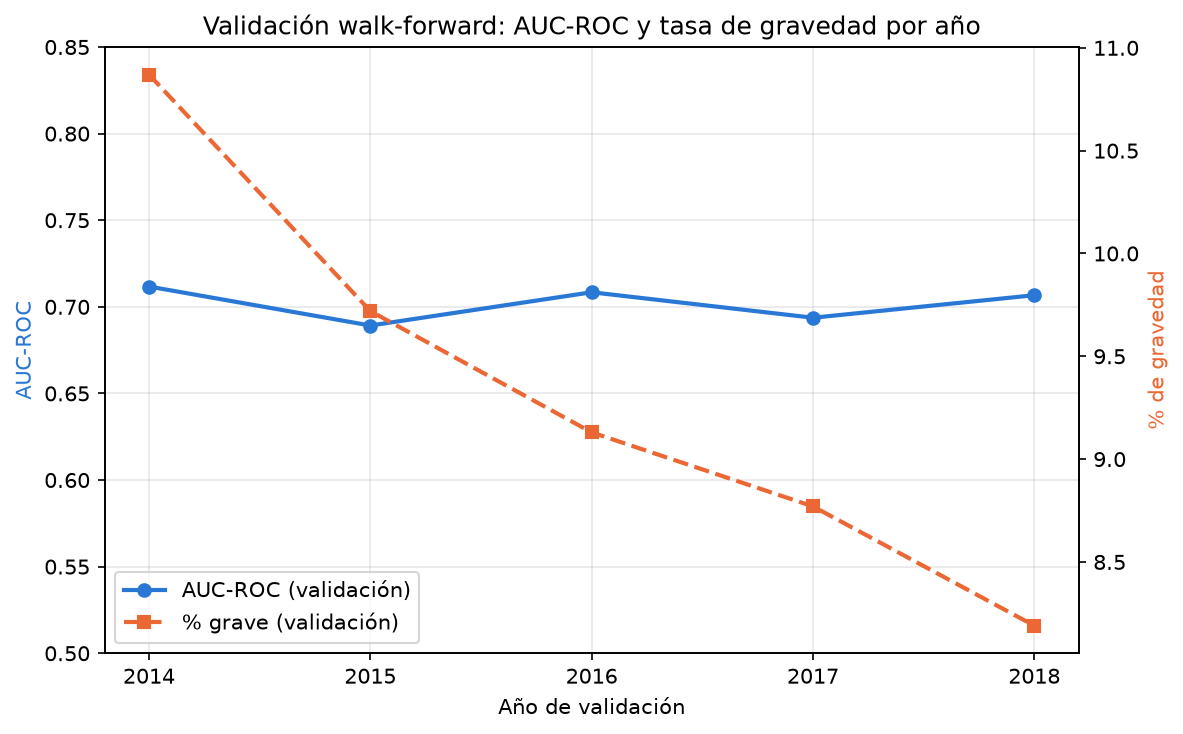
\includegraphics[width=0.72\textwidth]{../figures/14_validacion_walkforward.png}
\caption{Validación de ventana expansiva (2014--2018): el área bajo la curva ROC se mantiene estable pese al descenso sostenido de la tasa de gravedad real.}
\label{fig:walkforward}
\end{figure}

\subsection{Modelo explicativo y comparación entre preguntas}

¿Qué significa ``elegir el mejor modelo'' cuando el objetivo ya no es desplegarlo, sino interpretarlo? La interpretabilidad no es gratuita: los valores SHAP y los \emph{odds ratios} de la Sección~5 solo son fiables si vienen de un modelo que realmente aprendió las relaciones de los datos --- explicar un mal modelo produce patrones espurios, no hallazgos. Por eso se entrenan los mismos cuatro algoritmos, esta vez con su configuración por defecto y sin ninguna rejilla (tunear aquí rompería la comparación en igualdad de condiciones), y se elige el que mejor generaliza para servir de base a la interpretación. Tampoco basta con una regresión logística, pese a ser interpretable por diseño: un modelo lineal puede no captar relaciones no lineales, como el efecto de composición de la Sección~5.2. Por eso se elige el algoritmo ganador para la interpretación principal, manteniendo la regresión logística en paralelo como contraste (Sección~5.1): que dos modelos tan distintos coincidan en qué variables dominan respalda que el hallazgo es real, no un artefacto de un único algoritmo.

El modelo explicativo, entrenado con la matriz de referencia (42 variables, incluido el perfil de personas), se evaluó con los mismos cuatro candidatos. De nuevo \emph{Gradient Boosting} gana (AUC-ROC 0,722), seguido de la regresión logística (0,711); \emph{Random Forest} y XGBoost, sin tunear para esta matriz, sobreajustan marcadamente (0,691 y 0,688, con gap de 0,309 y 0,188) --- coherente con la Sección~4.2 sobre limitar su complejidad.

\begin{table}[h]
\centering
\small
\begin{tabular}{lcc}
\toprule
\textbf{Modelo} & \textbf{AUC-ROC} & \textbf{Gap train-test} \\
\midrule
\textbf{Gradient Boosting} & \textbf{0,722} & 0,061 \\
Regresión logística & 0,711 & 0,008 \\
\emph{Random Forest} & 0,691 & 0,309 (sobreajuste marcado) \\
XGBoost & 0,688 & 0,188 (sobreajuste marcado) \\
\bottomrule
\end{tabular}
\caption{Comparación de los cuatro modelos explicativos, sin ajuste de hiperparámetros (matriz de referencia, 42 variables).}
\label{tab:comparacion_explicativo}
\end{table}

Frente al mejor modelo operativo (XGBoost, 0,707), la mejora es real pero modesta: ~1,4 puntos de AUC-ROC. Las variables del momento del aviso ya capturan la mayor parte de la señal; el perfil de personas aporta valor incremental sin ser dominante --- su valor está más en la \textbf{interpretación para prevención} que en la mejora bruta de predicción.

% =============================================================================
\section{Interpretabilidad y hallazgos para la prevención}
% =============================================================================

\subsection{Metodología}

La idea central de los valores SHAP (\emph{SHapley Additive exPlanations}) es repartir el resultado de cada predicción entre las variables que la explican. Descomponen cada predicción en la contribución de cada variable, en la escala logarítmica del modelo (\emph{log-odds}); para traducir esa contribución a puntos de probabilidad hace falta partir del punto base real del explicador, no de la tasa media bruta, porque el modelo se entrena con ponderación de clases. Para validar que los hallazgos no dependen de un único algoritmo, se entrenó además una regresión logística cuyos coeficientes se leen como razones de probabilidades (\emph{odds ratios}): que dos modelos tan distintos coincidan en qué variables dominan refuerza que el hallazgo es real, no un artefacto de un algoritmo (funciones en el Anexo~\ref{app:interpretabilidad}).

\subsection{Factores de mayor peso}

\begin{table}[h]
\centering
\small
\begin{tabular}{lcc}
\toprule
\textbf{Variable} & \textbf{Contribución SHAP media} & \textbf{Puntos de probabilidad (aprox.)} \\
\midrule
Presencia de motocicleta/ciclomotor & 0,617 & 15,2 \\
Presencia de peatón & 0,304 & 7,4 \\
Número de víctimas (log) & 0,169 & 4,1 \\
Tipo de accidente = atropello & 0,147 & 3,5 \\
Hora del día (componente coseno) & 0,138 & 3,3 \\
\% histórico de motos en el distrito & 0,114 & 2,7 \\
Presencia de lluvia & 0,099 & 2,4 \\
Número de personas implicadas & 0,092 & 2,2 \\
Presencia de bicicleta & 0,085 & 2,1 \\
Hora del día (componente seno) & 0,083 & 2,0 \\
\bottomrule
\end{tabular}
\caption{Diez variables con mayor contribución media absoluta al riesgo predicho (escala SHAP en log-odds y su equivalente aproximado en puntos de probabilidad).}
\label{tab:shap}
\end{table}

La presencia de una motocicleta o ciclomotor es, con diferencia, la variable de mayor peso --- más del doble que la segunda--- seguida del peatón (tabla~\ref{tab:shap}): ambos son usuarios de la vía sin protección estructural frente a un impacto, a diferencia de ir en un turismo. La regresión logística confirma la jerarquía: la moto tiene la razón de probabilidades más alta del modelo (4,72, multiplica por 4,7 las probabilidades de gravedad), y el atropello la segunda entre las variables de riesgo directamente accionables (3,22) --- el número de víctimas (log), discutido aparte a continuación por no ser accionable, y el vuelco (poco frecuente, con intervalo de confianza más amplio) tienen una razón de probabilidades intermedia entre ambas.

Un matiz de SHAP: la contribución del atropello (0,147) es menor que la del peatón (0,304), aunque un atropello implica un peatón casi por definición --- sugiere que ``presencia de peatón'' capta algo más amplio, como un peatón golpeado en una colisión múltiple no clasificada como atropello.

El número de víctimas (log) aparece tercero, pero con cautela: al ser la gravedad el máximo entre implicados, más víctimas implica casi por construcción más probabilidad de que alguna sea grave. No es un hallazgo accionable, sino un reflejo del diseño de la variable objetivo --- por eso no se usa en el modelo operativo.

¿Por qué el número de personas implicadas no tiene una relación monótona con la gravedad? Una persona: 8,8\,\%; dos personas: 10,7\,\% (la más alta); tres o más: 9,0\,\% --- diferencia significativa (Mann-Whitney y chi-cuadrado, $p<0{,}001$; código en el Anexo~\ref{app:interpretabilidad}). Es un \textbf{efecto de composición}, no una relación causal: cada grupo está dominado por un tipo de accidente distinto.

\begin{itemize}[nosep]
\item \textbf{Una persona:} caídas de un único vehículo (moto, bici, ciclomotor) --- gravedad moderada (6,9--9,1\,\%).
\item \textbf{Dos personas:} colisión doble y, sobre todo, la configuración habitual del atropello (peatón + vehículo) --- gravedad mucho más alta (19,7\,\%), que arrastra la media del grupo.
\item \textbf{Tres o más:} dominado por la colisión múltiple, con gravedad baja (5,3\,\%) pese a más implicados, que diluye los atropellos de 3+ personas (27,8\,\%, el valor más alto de toda la tabla).
\end{itemize}

El número de personas no aumenta ni reduce el riesgo por sí mismo: lo que cambia es la mezcla de tipos de accidente que compone cada grupo --- coherente con que tipo de accidente ya es, en la tabla~\ref{tab:cramer}, la tercera variable con mayor asociación individual.

La Figura~\ref{fig:beeswarm} muestra, para las variables de la tabla~\ref{tab:shap}, cómo se distribuye su contribución en función de si la variable toma un valor alto (rojo) o bajo (azul) en cada accidente de la muestra.

\begin{figure}[h]
\centering
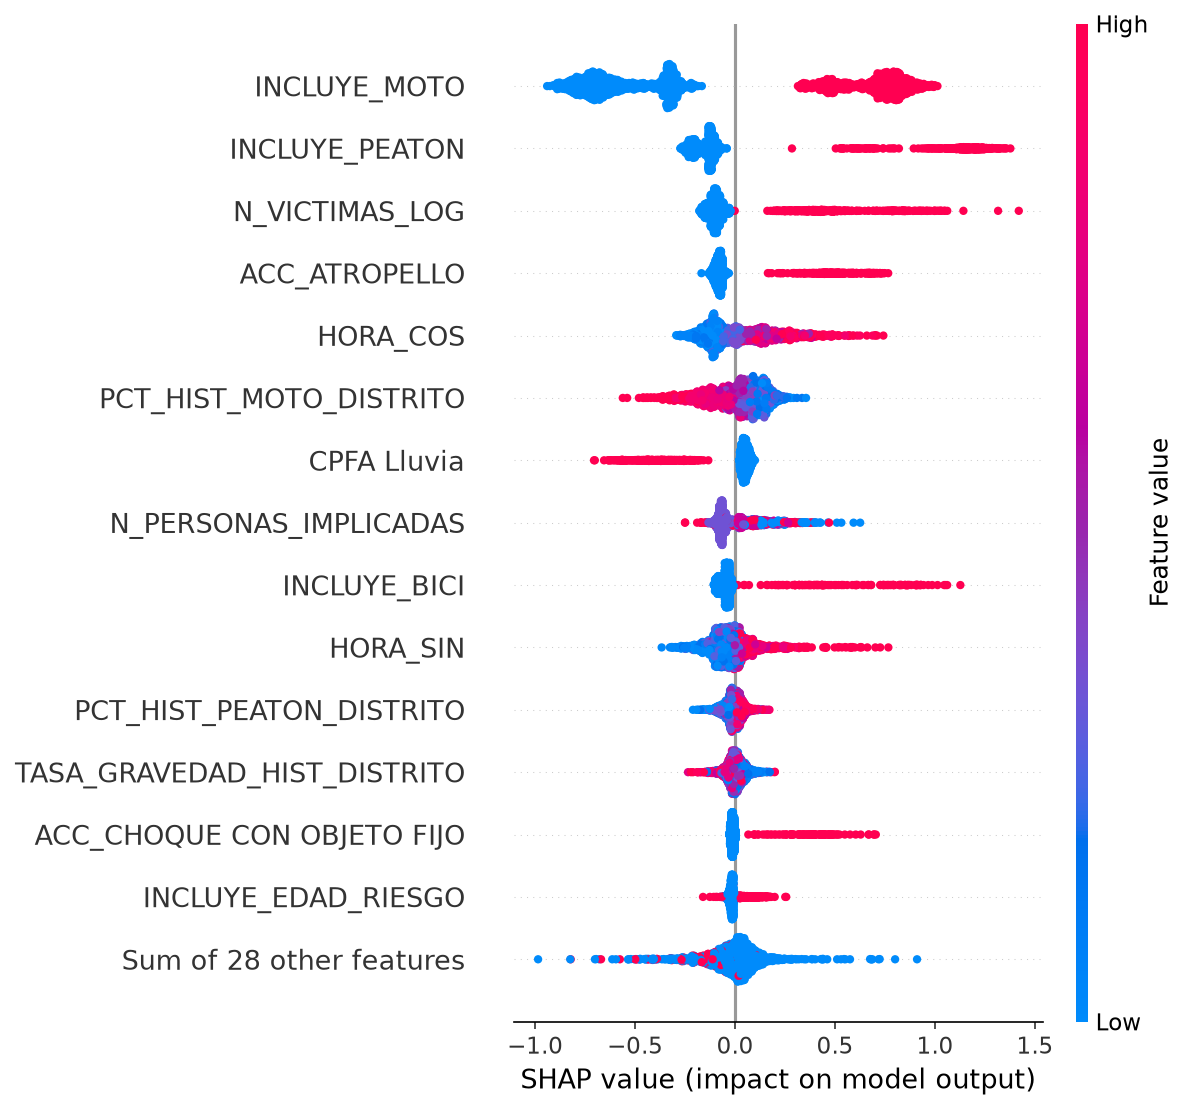
\includegraphics[width=0.72\textwidth]{../figures/16_shap_beeswarm.png}
\caption{Contribución de las variables más relevantes a la predicción de gravedad (cada punto es un accidente; rojo indica valor alto de la variable, azul valor bajo).}
\label{fig:beeswarm}
\end{figure}

\subsection{Focalización geográfica, temporal y demográfica}
\label{sec:focalizacion}

Para las tres dimensiones de focalización planteadas como objetivo se obtuvieron los siguientes resultados.

\textbf{Geográfica.} La contribución media de cada distrito al riesgo predicho no sigue el mismo orden que su tasa histórica bruta (compárese con la figura~\ref{fig:tasa_distrito}): Chamartín, Moncloa-Aravaca y Salamanca empujan más la predicción hacia mayor gravedad pese a una tasa moderada (~9\,\%), mientras que Vicálvaro, San Blas y Villa de Vallecas, con tasa más alta (10,7--11,7\,\%), quedan con contribución negativa (tabla~\ref{tab:distritos}). El motivo: el modelo ya explica buena parte del riesgo bruto de estos últimos vía otras variables (tipo de accidente, tipo de vehículo), así que su contribución \emph{incremental} --- una vez descontado lo demás--- es menor. Para focalizar por el riesgo que el modelo no atribuye ya a otro factor, los distritos prioritarios son los primeros, no los de mayor tasa bruta --- aunque el tamaño de muestra por distrito (33--168 accidentes) es limitado, y esta priorización es orientativa.

\begin{table}[h]
\centering
\small
\begin{tabular}{lccc}
\toprule
\textbf{Distrito} & \textbf{Contribución SHAP media} & \textbf{Tasa histórica bruta} & \textbf{Accidentes en la muestra} \\
\midrule
Chamartín & $+0{,}043$ & 9,1\,\% & 148 \\
Moncloa-Aravaca & $+0{,}041$ & 8,9\,\% & 109 \\
Salamanca & $+0{,}037$ & 9,0\,\% & 168 \\
\multicolumn{4}{c}{\dots} \\
Villa de Vallecas & $-0{,}032$ & 10,7\,\% & 53 \\
San Blas & $-0{,}052$ & 10,8\,\% & 105 \\
Vicálvaro & $-0{,}058$ & 11,7\,\% & 40 \\
\bottomrule
\end{tabular}
\caption{Distritos con la contribución SHAP media más alta y más baja, frente a su tasa histórica bruta de gravedad.}
\label{tab:distritos}
\end{table}

\textbf{Temporal.} La madrugada (0--7h, pico en torno a las 6) es la franja que más empuja hacia mayor gravedad; de 9h a media tarde el efecto es negativo, y vuelve a subir desde las 21h (figura~\ref{fig:shap_hora}). Coincide con el patrón ya visto en el EDA de forma puramente descriptiva (figura~\ref{fig:heatmap_gravedad}) --- confirmado por dos vías independientes--- y sugiere concentrar controles y campañas (velocidad, alcohol, fatiga) en el tramo nocturno.

\begin{figure}[h]
\centering
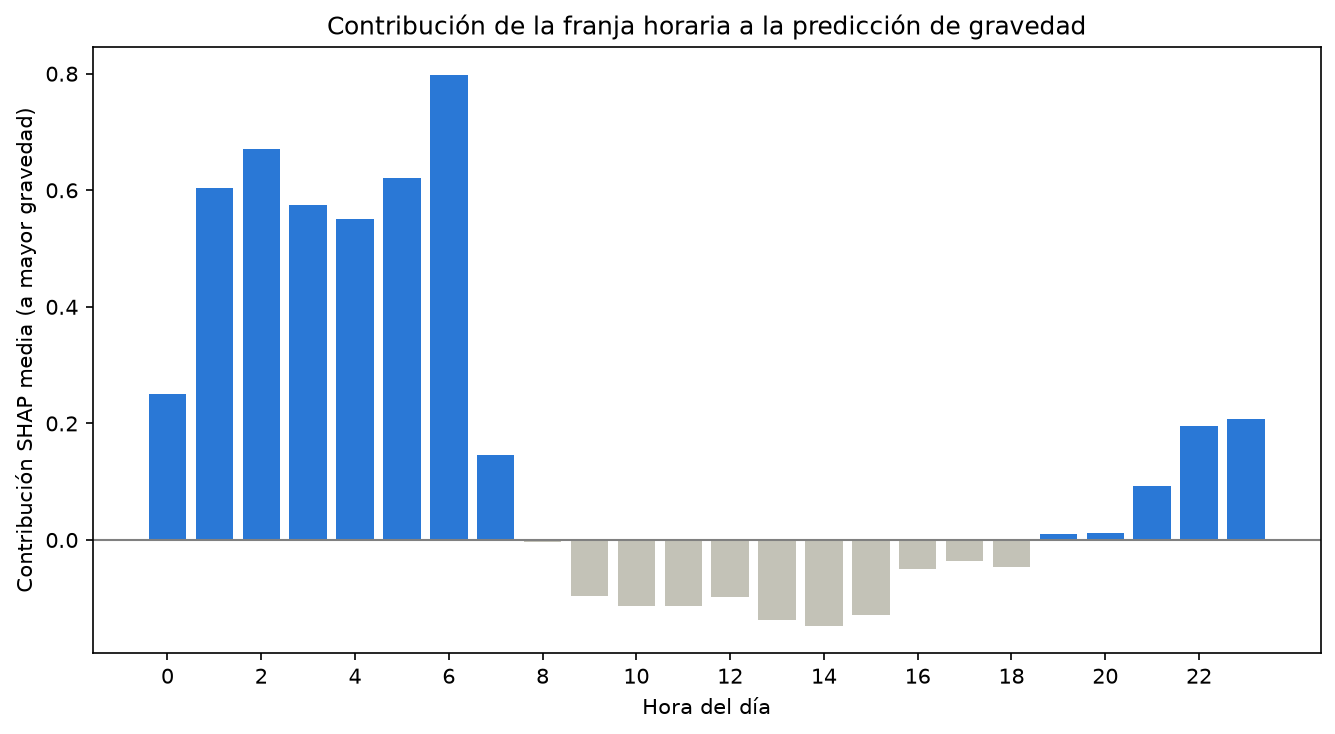
\includegraphics[width=0.75\textwidth]{../figures/18_shap_hora.png}
\caption{Contribución SHAP media de la franja horaria a la predicción de gravedad, por hora del día.}
\label{fig:shap_hora}
\end{figure}

\textbf{Demográfica.} La presencia de un menor o un mayor de 65 años muestra una contribución sistemáticamente positiva al riesgo (0,02--0,19 en log-odds) cuando está presente, y ligeramente negativa cuando no (figura~\ref{fig:shap_edad}). Es un efecto más modesto que el de motos o peatones, pero consistente en dirección --- apoya campañas dirigidas a estos colectivos, independientes del tipo de vehículo.

\begin{figure}[h]
\centering
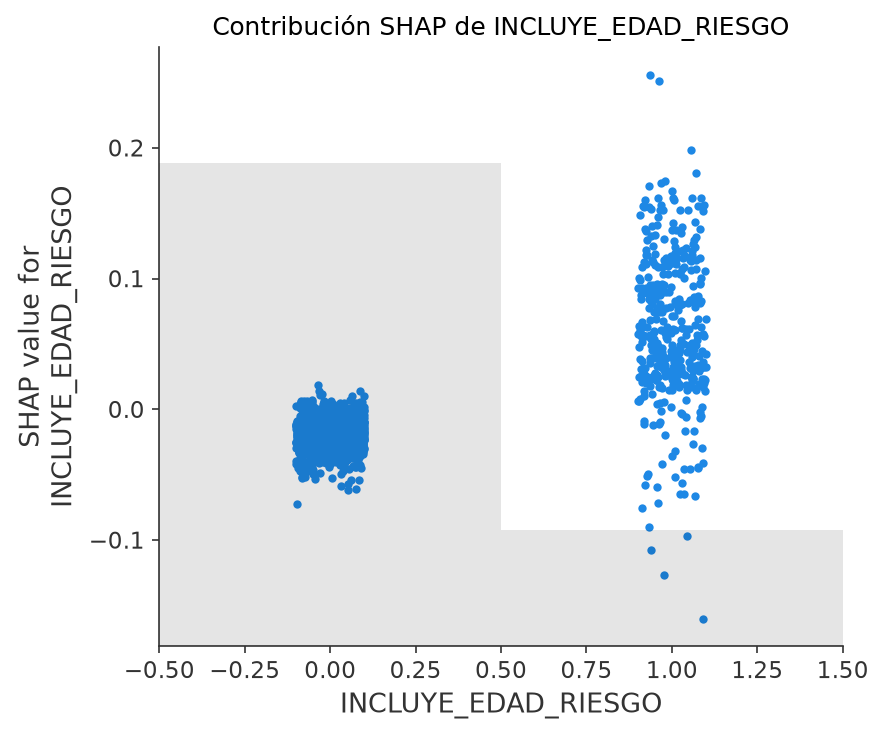
\includegraphics[width=0.6\textwidth]{../figures/19_shap_edad_riesgo.png}
\caption{Contribución SHAP de \texttt{INCLUYE\_EDAD\_RIESGO} (presencia de un menor o un mayor de 65 años), según esté ausente (0) o presente (1).}
\label{fig:shap_edad}
\end{figure}

En conjunto, moto, peatón y atropello no son ``prohibibles'' por una campaña, pero informan \textbf{dónde y cuándo} reforzar la protección de esos usuarios vulnerables: distrito, franja horaria y edad son la traducción operativa de estos hallazgos para campañas dirigidas, en vez de genéricas.

% =============================================================================
\section{Productivización}
% =============================================================================

Apoyar una decisión operativa exige que el modelo esté disponible en el momento en que esa decisión se toma, no solo en un análisis retrospectivo. Por ello, más allá del propio análisis, el trabajo incluye un pipeline reutilizable y una aplicación funcional, en línea con el objetivo de que el modelo de triaje pueda integrarse como apoyo real a la decisión operativa.

\subsection{Herramientas, control de versiones y estructura del repositorio}

Todo el proyecto se ha desarrollado en Visual Studio Code, con la extensión de Jupyter para trabajar los notebooks y control de versiones integrado con Git. El código completo --- notebooks, código fuente, configuración, aplicación web, scripts de productivización, memoria e informe de prevención--- está versionado y alojado públicamente en GitHub, en \url{https://github.com/meritxellabellan29/TFM-accidentes-trafico}, lo que permite consultar el historial de cambios, revisar el código fuente completo y clonar el repositorio para reproducir el proyecto de extremo a extremo.

El repositorio sigue una arquitectura por capas, separando claramente el análisis exploratorio del código reutilizable y de los artefactos de despliegue:

\begin{itemize}[itemsep=2pt]
\item \texttt{config/}: parámetros del proyecto en ficheros YAML (rutas, columnas requeridas, hiperparámetros de partición, artefactos de producción), leídos por \texttt{src/config.py} en lugar de estar escritos directamente en el código.
\item \texttt{data/}: datos originales (\texttt{raw/}) y datos ya limpios, transformados y con las matrices de variables (\texttt{processed/}, \texttt{processed/features/}).
\item \texttt{notebooks/}: los seis notebooks numerados del análisis (01\_EDA a 06\_Prediccion\_Nuevos\_Datos), que documentan el razonamiento paso a paso pero importan toda la lógica reutilizable desde \texttt{src/}, sin duplicarla.
\item \texttt{src/}: el código fuente reutilizable --- \texttt{pipelines/} (limpieza, preprocesado, feature engineering y la clase \texttt{PipelineAccidentes} de producción), \texttt{models/} (entrenamiento y evaluación) y \texttt{utils/} (gráficos e interpretabilidad).
\item \texttt{models/}: los modelos y el pipeline ya ajustados y serializados (\texttt{.joblib}), listos para cargarse sin reentrenar.
\item \texttt{scripts/}: puntos de entrada de producción independientes del notebook (predicción por línea de comandos, demo local, generación del informe de prevención, sincronización con la webapp).
\item \texttt{webapp/}: la aplicación Flask de triaje operativo, desplegable de forma independiente.
\item \texttt{reports/} y \texttt{figures/}: los artefactos generados --- el informe de prevención y todas las figuras del análisis y la memoria.
\item \texttt{memoria/}: este documento, en \LaTeX.
\end{itemize}

Esta separación es lo que permite que el mismo código se reutilice sin duplicación entre el análisis exploratorio, la aplicación web, el script de predicción por lotes y el informe de prevención, y es también lo que hace posible la reproducibilidad descrita en la Sección~\ref{sec:reproducibilidad}: cualquier persona con acceso al repositorio puede clonarlo, instalar las dependencias de \texttt{requirements.txt} y ejecutar cualquiera de esas piezas de forma independiente.

\subsection{Arquitectura del pipeline}

Toda la limpieza, el preprocesado y la ingeniería de variables se encapsulan en una única clase con una interfaz de ajuste y transformación, equivalente a la de las librerías estándar de aprendizaje automático: se ajusta una vez sobre el histórico --- aprendiendo y guardando internamente el mapeo de codificación del distrito, las categorías de tipo de vía y de accidente vistas, y sus categorías de referencia--- y después se aplica, sin volver a calcular nada de eso, tanto a nuevos lotes de datos como a un accidente individual descrito por sus características básicas (distrito, fecha y hora, tipo de vía y de accidente, condiciones, y opcionalmente si hay una moto o una bicicleta implicada). Ante una categoría no vista en el histórico de ajuste --- un distrito o un tipo de vía nuevo, por ejemplo--- el sistema no falla: la trata como la categoría más frecuente y lo notifica explícitamente por consola, en lugar de romper la predicción con un error críptico.

\subsection{La aplicación de triaje operativo}

La pieza central de la productivización es una \textbf{aplicación web}, con un formulario y una API de tipo REST, construida específicamente para el caso de uso de la Pregunta 1: apoyar a los servicios de emergencia en el momento del aviso. La persona que atiende la llamada al 112 introduce en el formulario los datos que ya conoce en ese instante (distrito, fecha y hora, tipo de vía, tipo de accidente, condiciones meteorológicas y del firme, y si se sabe que hay una moto o una bicicleta implicada) y la aplicación devuelve al momento la probabilidad de gravedad estimada por el modelo operativo (figura~\ref{fig:webapp}), sin exponer en ningún momento detalles técnicos del modelo. Nótese que es siempre el \textbf{modelo operativo} el que responde aquí --- nunca el explicativo--- precisamente porque es el único de los dos entrenado exclusivamente con información disponible en el momento del aviso, tal y como exige el caso de uso real. La función que traduce estos datos del formulario en la probabilidad devuelta se reproduce en el Anexo~\ref{app:predecir_individual}.

\begin{figure}[h]
\centering
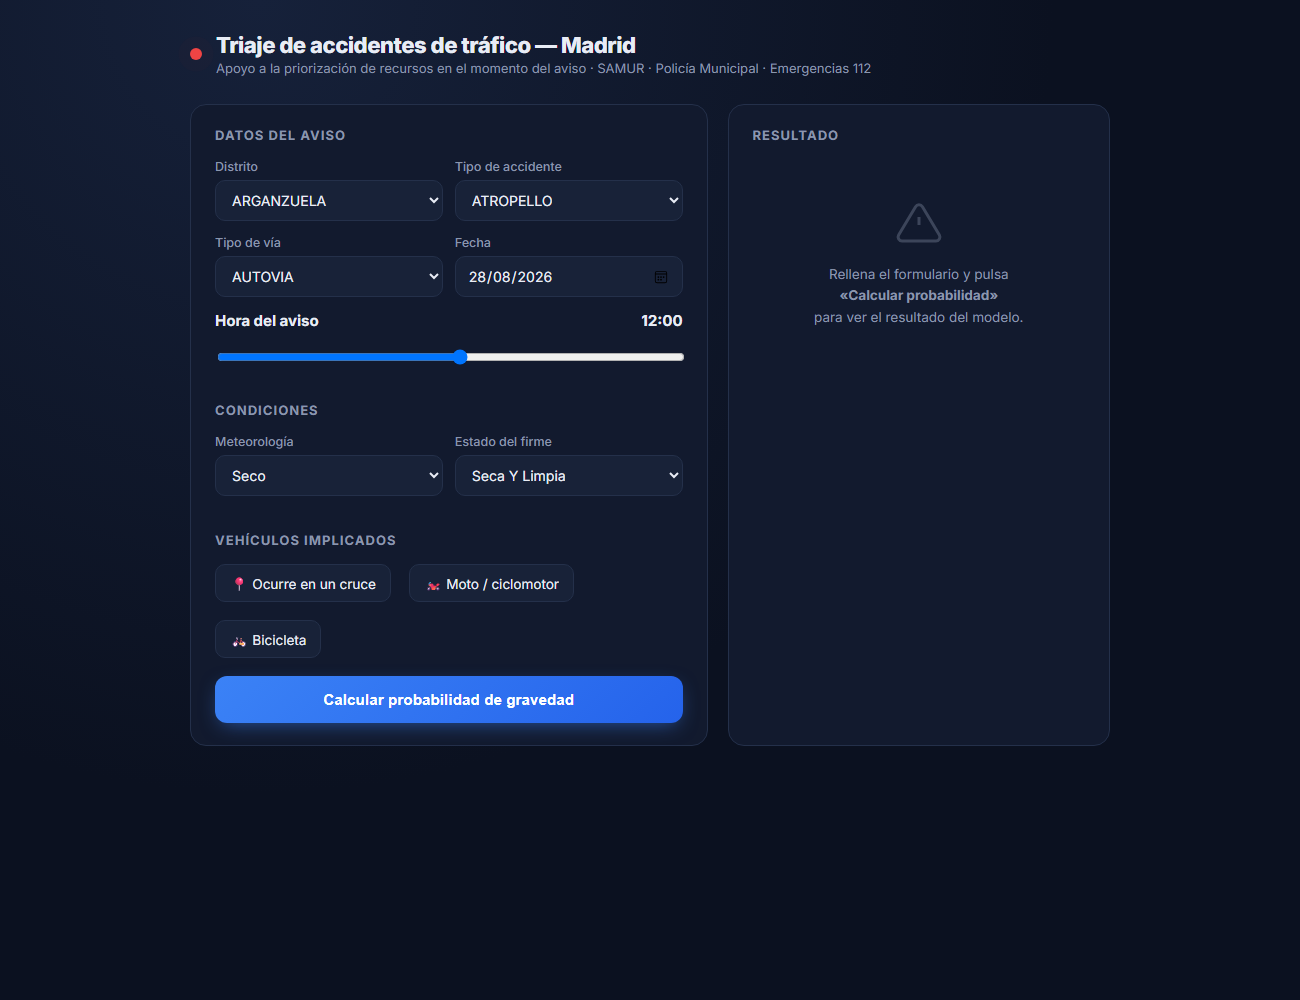
\includegraphics[width=0.62\textwidth]{../figures/20_webapp_formulario.png}
\caption{Formulario de la aplicación de triaje operativo, con un caso de ejemplo ya rellenado.}
\label{fig:webapp}
\end{figure}

Sobre esa probabilidad, la aplicación añade una capa ligera de reglas de negocio que traduce el porcentaje --- junto con el tipo de accidente y si hay una moto o una bicicleta implicada--- en una sugerencia de qué recursos reforzar: Policía Municipal siempre, para la regulación del tráfico y el atestado; SAMUR con carácter reforzado si la probabilidad de gravedad es alta o si hay un usuario vulnerable de la vía implicado; y Bomberos, ante una posible necesidad de excarcelación, en vuelcos o colisiones múltiples con probabilidad alta. Esta capa es intencionadamente de reglas y no una salida del modelo, porque el histórico de accidentes no registra qué recursos se enviaron a cada uno, así que no hay con qué entrenar esa predicción; el 112 no aparece como una alternativa más en la lista porque es el canal de coordinación a través del cual se despachan los demás, no un recurso que se decida activar o no. Esta función se reproduce en el Anexo~\ref{app:recursos}.

Sobre la misma clase de pipeline, y sin duplicar ninguna lógica de negocio entre ellas, se construyeron además otras dos formas de uso: un \textbf{script de línea de comandos} que procesa un fichero completo de accidentes nuevos y devuelve la probabilidad de gravedad de cada uno --- junto con el área bajo la curva ROC resultante, si la gravedad real ya es conocida--- útil para revalidar el modelo sobre datos futuros del mismo formato sin necesidad de abrir ningún notebook; y una \textbf{aplicación local} equivalente a la web, orientada a pruebas rápidas sin necesidad de desplegar nada.

Las opciones que se ofrecen en el formulario --- lista de distritos, de tipos de vía y de tipos de accidente--- se derivan dinámicamente del propio pipeline ya ajustado: si el modelo se reentrena en el futuro con más categorías o con distritos nuevos, el formulario se actualiza solo, sin tener que tocar el código de la aplicación.

\subsection{Informe de apoyo a la prevención vial}

Si la aplicación web productiviza el modelo operativo (Pregunta 1), el análisis de interpretabilidad (Pregunta 2) se productiviza en un \textbf{informe en PDF} para un público no técnico --- las autoridades de seguridad vial--- generado automáticamente por \texttt{scripts/generar\_informe\_prevencion.py} sin copiar ningún número a mano. Traduce los hallazgos de la Sección~5 a un formato visual, una página por bloque (factores de riesgo, franja horaria, focalización geográfica), con una cifra y una recomendación por hallazgo. Para que las cifras sean sólidas ante un público sin formación técnica, prioriza tasas observadas directamente en los datos sobre las probabilidades del modelo explicativo (que, al usar ponderación de clases, no son directamente comparables con la tasa real); la única excepción es la sección de distritos, donde el hallazgo --- qué distritos concentran más riesgo del que su contexto explicaría--- solo existe controlando esas otras variables.

\subsection{Reproducibilidad y escalabilidad a otros entornos}
\label{sec:reproducibilidad}

El pipeline no se limita al caso de Madrid: está pensado para aplicarse, con cambios mínimos, a datos de accidentalidad de otras ciudades que publiquen un formato equivalente (nivel persona, con lesividad, lugar, momento y condiciones) --- un escenario realista, ya que varios ayuntamientos y comunidades publican datos abiertos con estructura similar. Para que sea viable en la práctica se incorporaron dos salvaguardas (Anexo~\ref{app:validacion_esquema}):

\begin{itemize}[nosep]
\item \textbf{Validación de esquema:} comprueba al cargar los datos que están todas las columnas necesarias, y falla de inmediato con un mensaje explícito --- en vez de un error críptico varias funciones más abajo--- si el fichero nuevo tiene alguna columna renombrada o ausente.
\item \textbf{Diagnóstico de valores ``sin dato'':} revisa si aparecen convenciones de texto no reconocidas (antes de normalizar nulos) para decidirlo explícitamente, en vez de dejarlas pasar en silencio como una categoría más y sesgar el resultado sin aviso.
\end{itemize}

Además, todas las rutas y parámetros de partición (año de corte, tamaño de prueba, suavizado del agregado de distrito) se leen de ficheros de configuración externos, no del código, así que el pipeline puede reejecutarse sobre otro fichero o con otros parámetros sin tocar el código fuente. Trasladarlo a otra ciudad exigiría adaptar solo las piezas específicas de Madrid (categorías de distrito, clasificación de tipo de vía por palabras clave); el resto (limpieza, target encoding, codificación cíclica, detección de variable ficticia, entrenamiento y validación) es directamente reutilizable.

% =============================================================================
\section{Conclusiones y trabajo futuro}
% =============================================================================

\subsection{Conclusiones}

El trabajo responde a sus dos preguntas con resultados concretos.

\textbf{Triaje operativo (Pregunta 1).} XGBoost, entrenado solo con información del momento del aviso, alcanza un área bajo la curva ROC de 0,707 sobre un año no visto, estable en cinco años de validación. En términos honestos: 0,5 es azar puro y solo por encima de 0,8--0,9 se considera fuertemente discriminativo, así que 0,707 queda en el extremo inferior de lo ``aceptable'' --- mejor que no usar ningún modelo, pero lejos de un predictor determinante. Es coherente con el problema: falta toda la dinámica real del impacto (velocidad, mecanismo, factores humanos) que probablemente concentra la señal que el modelo no puede ver. El modelo explicativo, con más variables, solo mejora hasta 0,722 (Sección~4.5) --- confirma que el techo de rendimiento es del propio dataset, no una limitación específica del modelo operativo. Por eso el encuadre correcto, el que adopta la aplicación de demostración, es el de una señal de apoyo, nunca un sustituto del juicio profesional.

\textbf{Prevención vial (Pregunta 2).} El análisis de interpretabilidad --- contrastado con dos modelos distintos--- identifica motocicletas y peatones como los factores de mayor peso individual, y traduce el resto en recomendaciones de focalización:

\begin{itemize}[nosep]
\item \textbf{Dónde:} Chamartín, Moncloa-Aravaca y Salamanca, por su contribución incremental al riesgo más allá de lo ya explicado por otras variables.
\item \textbf{Cuándo:} la franja de madrugada, por su contribución sistemáticamente más alta.
\item \textbf{Quién:} menores y mayores de 65 años, como línea de prevención independiente del tipo de vehículo.
\end{itemize}

La diferencia de rendimiento entre ambos modelos (~1,4 puntos de AUC-ROC) confirma que restringirse a la información del aviso tiene un coste real pero moderado, y que el perfil de las personas vale más para interpretar que para predecir.

\subsection{Limitaciones}

La más relevante de cara a un uso operativo real es la baja precisión al umbral de 0,5: solo el 13,2\,\% de las alertas de gravedad alta son realmente graves (matriz de confusión, Sección~4.4). No es un defecto aislado, sino tres factores estructurales que conviene distinguir, porque cada uno exige una respuesta distinta:

\begin{itemize}[nosep]
\item \textbf{Desequilibrio de clases} (solo 9,6\,\% graves): una tasa moderada de falsos positivos entre los muchos accidentes leves (41,4\,\%) supera en número absoluto a los aciertos --- visible en el modesto AUC-PR (0,174) frente al AUC-ROC (0,707) de la tabla~\ref{tab:comparacion_operativo}. La brecha no es casual: el ROC mide falsos positivos \emph{sobre el total de negativos}; precisión-recall mide precisión \emph{sobre el total de positivos predichos} --- la pregunta que le importa a quien recibe la alerta.
\item \textbf{Ponderación de clases} en el entrenamiento --- necesaria para que el modelo no colapse prediciendo siempre ``no grave''--- desplaza el umbral efectivo y prioriza sensibilidad sobre precisión: razonable para un triaje (un falso negativo cuesta más que una alerta de más), pero hay que comunicarlo con claridad a quien use la herramienta.
\item \textbf{Techo de discriminación del modelo} (AUC-ROC 0,707): las distribuciones de graves y no graves se solapan bastante, así que cualquier umbral que capture la mayoría de los graves reales capturará también muchos que no lo son.
\end{itemize}

En un despliegue real, el umbral debería recalibrarse según el coste relativo de cada tipo de error, no mantenerse en 0,5.

Otras limitaciones reconocidas:

\begin{itemize}[nosep]
\item La clasificación del tipo de vía por reglas de texto es una aproximación razonable pero mejorable --- geocodificar permitiría cruzar con velocidad de vía real.
\item La validación de ventana expansiva no reajusta en cada iteración las variables aprendidas del histórico, por simplicidad, lo que podría favorecer ligeramente a los primeros años.
\item La deriva temporal en la tasa de gravedad implica que un despliegue real necesitaría recalibración periódica.
\item El tamaño de muestra por distrito en test es limitado, así que la priorización geográfica es orientativa.
\item El periodo de datos (2012--2018) no incluye el patinete eléctrico, hoy ya relevante para la seguridad vial de la ciudad; una actualización futura debería incorporarlo como categoría de vehículo.
\end{itemize}

\subsection{Trabajo futuro}

Como continuación natural de este trabajo se plantean:

\begin{itemize}[nosep]
\item Calibrar el umbral de decisión según el coste relativo de un falso negativo frente a una falsa alarma, en vez de mantener 0,5 por defecto.
\item Geocodificar la descripción del lugar del accidente para incorporar velocidad de vía real.
\item Explorar una validación de ventana expansiva que reajuste todas las transformaciones en cada iteración, sin dependencia del histórico completo.
\item Incorporar una estrategia explícita de recalibración periódica en el pipeline de producción.
\item Actualizar el modelo con datos más recientes que incluyan los nuevos medios de movilidad urbana (patinete eléctrico y similares).
\item Extender la aplicación de demostración con un panel de seguimiento para las instituciones de prevención vial, que muestre la evolución de las recomendaciones a medida que haya nuevos datos.
\end{itemize}

% =============================================================================
\section*{Bibliografía}
\addcontentsline{toc}{section}{Bibliografía}
% =============================================================================

\begin{enumerate}[nosep,leftmargin=1.3cm]
\item Ayuntamiento de Madrid. \emph{Portal de Datos Abiertos --- Accidentes de tráfico}. \url{https://datos.madrid.es}.
\item Lundberg, S. M., y Lee, S.-I. (2017). \emph{A Unified Approach to Interpreting Model Predictions}. Advances in Neural Information Processing Systems 30.
\item Chen, T., y Guestrin, C. (2016). \emph{XGBoost: A Scalable Tree Boosting System}. Proceedings of the 22nd ACM SIGKDD International Conference on Knowledge Discovery and Data Mining.
\item Pedregosa, F., et al. (2011). \emph{Scikit-learn: Machine Learning in Python}. Journal of Machine Learning Research, 12, 2825--2830.
\item Hastie, T., Tibshirani, R., y Friedman, J. (2009). \emph{The Elements of Statistical Learning} (2.ª ed.). Springer.
\item Lilliefors, H. W. (1967). \emph{On the Kolmogorov-Smirnov Test for Normality with Mean and Variance Unknown}. Journal of the American Statistical Association, 62(318), 399--402.
\end{enumerate}

\newpage
\appendix
\section{Código representativo del proyecto}

Este anexo recoge los fragmentos de código reales del proyecto que sostienen cada afirmación cuantitativa o decisión metodológica del cuerpo del documento. El código completo, con el resto de funciones, los seis notebooks y la aplicación web, está disponible en \url{https://github.com/meritxellabellan29/TFM-accidentes-trafico} (Sección~6.1; repositorio público, sin necesidad de permisos para consultarlo). Algunos fragmentos omiten, marcándolo explícitamente con un comentario, partes repetitivas del docstring original (por ejemplo, la documentación exhaustiva de cada parámetro) que no aportan a la comprensión del razonamiento; por legibilidad tipográfica dentro del bloque de código.

\subsection{Asociación estadística con corrección por comparaciones múltiples (\texttt{01\_EDA.ipynb})}
\label{app:cramer}

La función que calcula la V de Cramér de la tabla~\ref{tab:cramer} (Sección~2.8), junto con la corrección de Bonferroni aplicada antes de interpretar cualquier test de independencia chi-cuadrado como significativo.

\begin{lstlisting}[caption={Cálculo de la V de Cramér y corrección de Bonferroni para comparaciones múltiples.}]
from scipy.stats import chi2_contingency

# Correccion de Bonferroni: dividir el umbral de significancia habitual
# (0.05) entre el numero de variables testeadas, para no declarar
# "significativo" algo que solo lo parece por puro azar de probar muchas
# variables a la vez
alpha_corregido = 0.05 / len(vars_categoricas)

def cramers_v(x, y):
    """V de Cramer, corregida por sesgo (Bergsma 2013): mide la fuerza
    de la asociacion entre dos variables categoricas, entre 0 (ninguna)
    y 1 (perfecta) -- a diferencia del chi-cuadrado bruto, no depende
    del tamano de la muestra, lo que permite comparar variables con
    distinto numero de categorias entre si."""
    confusion_matrix = pd.crosstab(x, y)
    chi2, _, _, _ = chi2_contingency(confusion_matrix)
    n = confusion_matrix.sum().sum()
    r, k = confusion_matrix.shape
    phi2 = chi2 / n
    phi2corr = max(0, phi2 - ((k - 1) * (r - 1)) / (n - 1))
    rcorr = r - ((r - 1) ** 2) / (n - 1)
    kcorr = k - ((k - 1) ** 2) / (n - 1)
    denom = min((kcorr - 1), (rcorr - 1))
    if denom <= 0:
        return 0.0
    return np.sqrt(phi2corr / denom)

# Cada variable se testea en su nivel real de variacion (ver Seccion 2.7):
# las de persona contra el dataframe a nivel persona, las de accidente
# contra el dataframe ya agregado a nivel accidente -- para no
# pseudo-replicar cada accidente una vez por implicado
resultados = []
for var in vars_persona:
    mask = df_sin_na[var].notna() & df_sin_na['LESIVIDAD'].notna()
    v_gra = cramers_v(df_sin_na.loc[mask, var], df_sin_na.loc[mask, 'GRAVE'].astype(str))
    resultados.append({'Variable': var, 'Nivel': 'Persona', 'V_Grave': v_gra})

for var in vars_accidente:
    mask = df_accidentes[var].notna() & df_accidentes['accidente_grave'].notna()
    v_gra = cramers_v(df_accidentes.loc[mask, var], df_accidentes.loc[mask, 'accidente_grave'].astype(str))
    resultados.append({'Variable': var, 'Nivel': 'Accidente', 'V_Grave': v_gra})

df_cramer = pd.DataFrame(resultados).sort_values('V_Grave', ascending=False)
\end{lstlisting}

\subsection{De persona a accidente y clasificación del tipo de vía (\texttt{src/pipelines/preprocesado.py})}
\label{app:preprocesado}

Las funciones que transforman el dataset de nivel persona a nivel accidente (Sección~3.1): construyen los indicadores de implicación (\texttt{INCLUYE\_*}), verifican que las columnas ``de accidente'' realmente no varían dentro de un mismo accidente antes de asumirlo, y clasifican el tipo de vía a partir del texto libre del lugar.

\begin{lstlisting}[caption={Agregación de persona a accidente, verificación de invariancia y clasificación del tipo de vía por texto.}]
def agregar_flags_persona(df, df_pers, grupos_riesgo_edad=GRUPOS_RIESGO_EDAD):
    """Agrega de persona a accidente las variables de persona con mayor
    asociacion con la gravedad, como flags de implicacion, en vez de
    perderlas al agregar.

    N_PERSONAS_IMPLICADAS se calcula sobre `df` completo (no sobre
    `df_pers`), porque de lo contrario infraestimaria el numero real de
    implicados en cualquier accidente con alguna persona de LESIVIDAD
    desconocida (~8.9% de los accidentes)."""
    n_personas_real = df.groupby('Nº PARTE').size().rename('N_PERSONAS_IMPLICADAS')

    agg_flags = df_pers.groupby('Nº PARTE').agg(
        GRAVE=('GRAVE', 'max'),
        INCLUYE_PEATON=('TIPO PERSONA', lambda s: (s == 'PEATON').any()),
        INCLUYE_MOTO=('Tipo Vehiculo', lambda s: s.isin(['MOTOCICLETA', 'CICLOMOTOR']).any()),
        INCLUYE_BICI=('Tipo Vehiculo', lambda s: (s == 'BICICLETA').any()),
        INCLUYE_EDAD_RIESGO=('Tramo Edad', lambda s: s.isin(grupos_riesgo_edad).any()),
    ).reset_index()

    return agg_flags.merge(n_personas_real, on='Nº PARTE', how='left')


def verificar_invariancia_por_accidente(df, cols=COLS_ACCIDENTE):
    """Comprueba que las columnas "de accidente" (fecha, distrito,
    meteorologia...) no varian dentro de un mismo numero de parte, antes
    de asumirlo y tomar el primer valor sin mas. Devuelve un dict
    {columna: numero de accidentes inconsistentes} solo con las columnas
    que si presentan alguna inconsistencia."""
    inconsistencias = {
        c: (df.groupby('Nº PARTE')[c].nunique() > 1).sum()
        for c in cols if c != 'Nº PARTE'
    }
    return {k: v for k, v in inconsistencias.items() if v > 0}


def tipo_via(texto):
    """Clasifica LUGAR ACCIDENTE por tipo de via, usando todo el texto
    (no solo el primer tramo antes de un posible '-') con un orden de
    prioridad de mayor a menor velocidad/relevancia esperada. Si el
    cruce mezcla dos tipos (p. ej. 'CALLE - AUTOVIA'), prevalece el de
    mayor prioridad -- el orden de los tramos en el texto es alfabetico
    en ~88% de los casos, no indica cual via es la "principal"."""
    if pd.isna(texto):
        return np.nan
    t = texto.upper()
    if 'AUTOVIA' in t or 'M-30' in t or 'M-40' in t:
        return 'AUTOVIA'
    if 'CARRETERA' in t:
        return 'CARRETERA'
    if 'RONDA' in t:
        return 'RONDA'
    if 'AVENIDA' in t:
        return 'AVENIDA'
    if 'PASEO' in t:
        return 'PASEO'
    if 'GLORIETA' in t:
        return 'GLORIETA'
    if 'CALLE' in t:
        return 'CALLE'
    if 'PLAZA' in t:
        return 'PLAZA'
    return 'OTROS'


def detectar_cruce(df):
    """Anade ES_CRUCE: patron 'CALLE 1 - CALLE 2' en LUGAR ACCIDENTE,
    que marca una interseccion entre dos vias (~46% de los accidentes)."""
    df = df.copy()
    df['ES_CRUCE'] = df['LUGAR ACCIDENTE'].str.contains(' - ', na=False).astype(int)
    return df
\end{lstlisting}

\subsection{Target encoding suavizado, codificación cíclica y VIF (\texttt{src/pipelines/feature\_engineering.py})}
\label{app:encoding}

Las funciones que construyen el agregado histórico de distrito (con y sin fuga de información dentro de train), la codificación cíclica de hora y mes, y el cálculo del factor de inflación de la varianza (Sección~3.4-3.5).

\begin{lstlisting}[caption={Target encoding suavizado (con y sin fuga de información), codificación cíclica y VIF.}]
def smoothed_target_encode(train_df, col, target, m):
    """Codificacion de una categorica por la media (suavizada) de
    `target` en ese grupo, ajustada con TODO train. Se usa para el
    mapeo final que se aplica a test.

    El suavizado (parametro `m`) combina la tasa del grupo con la media
    global, ponderando por su tamano de muestra: un distrito con pocos
    accidentes y una tasa extrema por puro azar queda "tirado" hacia la
    media global, en vez de distorsionar el modelo con una senal poco
    fiable."""
    global_mean = train_df[target].mean()
    agg = train_df.groupby(col)[target].agg(['mean', 'count'])
    smoothed = (agg['count'] * agg['mean'] + m * global_mean) / (agg['count'] + m)
    return smoothed, global_mean


def smoothed_target_encode_oof(train_df, col, target, m, n_splits=5, random_state=42):
    """Version out-of-fold para TRAIN: cada fila se codifica con un
    mapeo aprendido en los folds a los que NO pertenece, para que no
    contribuya a su propio valor -- si no, cada fila "ve" un poco de su
    propia etiqueta a traves de la media de su grupo, una fuga de
    informacion sutil pero real."""
    from sklearn.model_selection import KFold
    kf = KFold(n_splits=n_splits, shuffle=True, random_state=random_state)
    oof = pd.Series(index=train_df.index, dtype=float)
    global_mean = train_df[target].mean()

    for idx_fit, idx_hold in kf.split(train_df):
        fit_fold = train_df.iloc[idx_fit]
        agg = fit_fold.groupby(col)[target].agg(['mean', 'count'])
        smoothed_fold = (agg['count'] * agg['mean'] + m * global_mean) / (agg['count'] + m)
        oof.iloc[idx_hold] = train_df.iloc[idx_hold][col].map(smoothed_fold).fillna(global_mean)

    return oof


def codificar_ciclica(df, col, periodo):
    """Codifica una variable ciclica (p. ej. HORA con periodo 24, MES
    con periodo 12) en seno/coseno, para no imponer un salto artificial
    en la frontera del ciclo (23h -> 0h, diciembre -> enero)."""
    df = df.copy()
    df[f'{col}_SIN'] = np.sin(2 * np.pi * df[col] / periodo)
    df[f'{col}_COS'] = np.cos(2 * np.pi * df[col] / periodo)
    return df


# Factor de inflacion de la varianza (VIF): cuanto se puede predecir
# cada variable a partir de TODAS las demas combinadas, no solo de otra
# tomada de dos en dos -- por eso complementa, y no sustituye, al
# cribado de correlaciones por pares
import statsmodels.api as sm
from statsmodels.stats.outliers_influence import variance_inflation_factor

X_vif = sm.add_constant(X_train_op.astype(float))
vif_df = pd.DataFrame({
    'variable': X_vif.columns,
    'VIF': [variance_inflation_factor(X_vif.values, i) for i in range(X_vif.shape[1])]
})
vif_df = vif_df[vif_df['variable'] != 'const'].sort_values('VIF', ascending=False)
\end{lstlisting}

\subsection{Validación de esquema y diagnóstico de valores ausentes (\texttt{src/pipelines/limpieza.py})}
\label{app:validacion_esquema}

Las dos funciones que sostienen la reproducibilidad frente a un Excel nuevo de otro año o de otra ciudad (Sección~6.5): fallar rápido y de forma legible si falta una columna esperada, y avisar si aparece una convención de ``sin dato'' que el sistema todavía no reconoce como tal.

\begin{lstlisting}[caption={Validación de esquema y diagnóstico de valores ``sin dato'' no reconocidos.}]
def validar_esquema(df, columnas_requeridas):
    """Comprueba que `df` tiene al menos las columnas de
    `columnas_requeridas`, y falla con un mensaje explicito si falta
    alguna -- en vez de un KeyError criptico varias funciones mas abajo."""
    columnas_faltantes = set(columnas_requeridas) - set(df.columns)
    if columnas_faltantes:
        raise ValueError(
            'El Excel cargado no tiene el formato esperado, faltan '
            f'columnas: {sorted(columnas_faltantes)}'
        )


def diagnosticar_valores_sin_dato_no_reconocidos(df, valores_conocidos=VALORES_NULOS):
    """Busca en las columnas de texto valores que parezcan representar
    "sin dato" (contienen palabras como DESCONOCIDO, NO ASIGNADO, N/D,
    NULL...) pero que NO esten en `valores_conocidos` -- es decir, que
    normalizar_nulos() dejaria pasar tal cual como una categoria mas, en
    vez de convertirlos en NaN.

    Devuelve un dict {columna: [valores sospechosos]}, vacio si no hay
    nada que revisar."""
    valores_conocidos_upper = {str(v).upper() for v in valores_conocidos}
    sospechosos = {}
    for col in df.select_dtypes(include=['object', 'string']).columns:
        encontrados = sorted({
            v for v in df[col].dropna().unique()
            if isinstance(v, str)
            and v.upper() not in valores_conocidos_upper
            and _PATRON_SIN_DATO_SOSPECHOSO.search(v)
        })
        if encontrados:
            sospechosos[col] = encontrados
    return sospechosos
\end{lstlisting}

\subsection{Predicción de un accidente individual (\texttt{src/pipelines/pipeline\_produccion.py})}
\label{app:predecir_individual}

La función que usa realmente la aplicación web (Sección~6.3): a partir únicamente de los datos que se conocerían en el momento del aviso, construye la misma fila de variables que vio el modelo en entrenamiento y llama a \texttt{predict\_proba} --- el mismo mecanismo, explicado en la Sección~4.1, por el que un modelo entrenado sobre una etiqueta binaria (grave/no grave) puede devolver un porcentaje.

\begin{lstlisting}[caption={Predicción de la probabilidad de gravedad de un accidente individual, a partir de los datos disponibles en el momento del aviso.}]
def predecir_accidente_individual(self, modelo, distrito, fecha_hora,
                                   tipo_accidente, tipo_via=None,
                                   lugar_texto=None, es_cruce=None,
                                   meteorologia='Seco',
                                   estado_firme='Seca Y Limpia',
                                   incluye_moto=False, incluye_bici=False):
    """Predice la probabilidad de gravedad de UN accidente a partir de
    los datos disponibles en el momento del aviso -- sin depender de
    LESIVIDAD ni de ningun dato de las personas implicadas (es el caso
    de uso real de la Pregunta 1, el que usa la webapp)."""
    # (documentacion completa de cada parametro omitida aqui, ver repositorio)
    assert self.ajustado, "El pipeline no esta ajustado."

    fecha_hora = pd.to_datetime(fecha_hora)
    hora, mes = fecha_hora.hour, fecha_hora.month
    es_finde = int(fecha_hora.dayofweek >= 5)

    if lugar_texto is not None:
        tipo_via_final = prep.tipo_via(lugar_texto)
        es_cruce_final = int(' - ' in lugar_texto.upper())
    else:
        tipo_via_final = tipo_via
        es_cruce_final = int(bool(es_cruce)) if es_cruce is not None else 0

    if tipo_via_final not in self.cats_tipo_via + [self.ref_via]:
        print(f"Aviso: TIPO_VIA '{tipo_via_final}' no vista en train "
              "-- se trata como la categoria de referencia.")

    fila = {}
    fila['ES_CRUCE'] = es_cruce_final
    fila['ES_FINDE'] = es_finde
    fila['HORA_SIN'] = np.sin(2 * np.pi * hora / 24)
    fila['HORA_COS'] = np.cos(2 * np.pi * hora / 24)
    fila['MES_SIN'] = np.sin(2 * np.pi * mes / 12)
    fila['MES_COS'] = np.cos(2 * np.pi * mes / 12)

    # Construye las columnas one-hot (meteorologia, firme, tipo de via,
    # tipo de accidente) comparando cada categoria posible con la
    # recibida -- exactamente el mismo esquema aprendido en fit()
    for col in self.features_operativo:
        if col.startswith('CPFA '):
            fila[col] = int(col == f'CPFA {meteorologia}')
        elif col.startswith('CPSV '):
            fila[col] = int(col == f'CPSV {estado_firme}')
        elif col.startswith('VIA_'):
            fila[col] = int(col == f'VIA_{tipo_via_final}')
        elif col.startswith('ACC_'):
            fila[col] = int(col == f'ACC_{tipo_accidente}')

    # Agregados historicos del distrito: se usa el mapeo ya aprendido en
    # fit() (nunca recalculado), con la media global como respaldo si el
    # distrito no se vio en entrenamiento
    for nuevo, (col, mapping, global_mean) in self.mapeos_encoding.items():
        fila[nuevo] = mapping.get(distrito, global_mean)

    fila['INCLUYE_MOTO'] = int(incluye_moto)
    fila['INCLUYE_BICI'] = int(incluye_bici)

    X_individual = pd.DataFrame([fila])[self.features_operativo]
    probabilidad = modelo.predict_proba(X_individual)[0, 1]

    return {
        'probabilidad_grave': round(float(probabilidad), 4),
        'inputs_interpretados': {
            'distrito': distrito, 'hora': hora, 'mes': mes,
            'es_finde': bool(es_finde), 'tipo_accidente': tipo_accidente,
            'tipo_via': tipo_via_final, 'es_cruce': bool(es_cruce_final),
            'meteorologia': meteorologia, 'estado_firme': estado_firme,
            'incluye_moto': bool(incluye_moto), 'incluye_bici': bool(incluye_bici),
        },
    }
\end{lstlisting}

\subsection{Rejilla de hiperparámetros y métricas de evaluación (\texttt{src/models/entrenamiento.py})}
\label{app:hiperparametros}

La función que ejecuta, para cada algoritmo, la rejilla manual de combinaciones descrita en la Sección~4.2, calculando el sobreajuste siempre contra la validación cruzada dentro de entrenamiento --- nunca contra el conjunto de prueba, para no filtrar información hacia la evaluación final --- seguida de las funciones que calculan las métricas de la tabla~\ref{tab:comparacion_operativo} y el ``gap train-test'' de la tabla~\ref{tab:fortalezas}.

\begin{lstlisting}[caption={Exploración manual de una rejilla de hiperparámetros, con validación temporal dentro de entrenamiento.}]
def explorar_hiperparametros(estimador_factory, grid, X_train, y_train, cv_splits=5):
    """Grid MANUAL y explicito (no distribuciones aleatorias): prueba
    cada combinacion exacta del `grid` dado, entrenando sobre TODO train
    y validando con TimeSeriesSplit -- todo dentro de train, sin tocar
    test en ningun momento de esta exploracion.

    El gap se calcula como AUC_train - AUC_cv (validacion cruzada dentro
    de train), NO como AUC_train - AUC_test: si se calculara el gap
    contra test para elegir entre combinaciones, se estaria mirando el
    test repetidamente para decidir -- la misma fuga de informacion que
    la validacion cruzada existe para evitar.

    Devuelve una tabla ordenada por AUC_cv descendente, con `AUC_cv_se`
    (error estandar entre folds) que permite aplicar la regla de "1 error
    estandar" (Hastie, Tibshirani y Friedman) al elegir configuracion: la
    mejor por AUC_cv no siempre es la mas adecuada si su ventaja esta
    dentro del ruido de la validacion cruzada."""
    from sklearn.model_selection import ParameterGrid, TimeSeriesSplit, cross_val_score

    cv = TimeSeriesSplit(n_splits=cv_splits)
    resultados = []

    for params in ParameterGrid(grid):
        modelo = estimador_factory(**params)
        scores_cv = cross_val_score(modelo, X_train, y_train,
                                     scoring='roc_auc', cv=cv, n_jobs=-1)
        auc_cv = scores_cv.mean()
        auc_cv_se = scores_cv.std(ddof=1) / np.sqrt(len(scores_cv))
        modelo.fit(X_train, y_train)
        auc_train = roc_auc_score(y_train, modelo.predict_proba(X_train)[:, 1])

        resultados.append({
            **params,
            'AUC_train': round(auc_train, 4),
            'AUC_cv': round(auc_cv, 4),
            'AUC_cv_se': round(auc_cv_se, 4),
            'gap_train_cv': round(auc_train - auc_cv, 4),
        })

    return pd.DataFrame(resultados).sort_values('AUC_cv', ascending=False)


def evaluar_modelo(modelo, X, y, umbral=0.5):
    """Calcula el conjunto de metricas relevante para un problema
    desbalanceado: AUC-ROC y AUC-PR (no dependen de un umbral), Brier
    score (calibracion), y precision/recall/F1 en el umbral dado (por
    defecto 0.5 -- recordar que con este nivel de desbalanceo, 0.5 puede
    no ser el mejor punto de corte para un uso real de priorizacion)."""
    y_proba = modelo.predict_proba(X)[:, 1]
    y_pred = (y_proba >= umbral).astype(int)
    return {
        'AUC-ROC': roc_auc_score(y, y_proba),
        'AUC-PR': average_precision_score(y, y_proba),
        'Brier score': brier_score_loss(y, y_proba),
        f'Precision (umbral={umbral})': precision_score(y, y_pred, zero_division=0),
        f'Recall (umbral={umbral})': recall_score(y, y_pred, zero_division=0),
        f'F1 (umbral={umbral})': f1_score(y, y_pred, zero_division=0),
    }


def tabla_comparativa_modelos(modelos, X_train, y_train, X_test, y_test, umbral=0.5):
    """Evalua varios modelos ya entrenados EN TRAIN Y EN TEST -- no solo
    en test -- para poder medir el gap train-test (sintoma de
    overfitting). Un modelo con AUC-ROC ~0.99 en train y ~0.75 en test
    esta sobreajustando, aunque su metrica de test por si sola parezca
    razonable."""
    filas = {}
    for nombre, modelo in modelos.items():
        m_train = evaluar_modelo(modelo, X_train, y_train, umbral=umbral)
        m_test = evaluar_modelo(modelo, X_test, y_test, umbral=umbral)
        fila = {f'{k}_train': v for k, v in m_train.items()}
        fila.update({f'{k}_test': v for k, v in m_test.items()})
        fila['gap_AUC-ROC'] = m_train['AUC-ROC'] - m_test['AUC-ROC']
        filas[nombre] = fila
    return pd.DataFrame(filas).T.round(4)
\end{lstlisting}

\subsection{Validaciones adicionales: estabilidad del bagging, deriva temporal y ventana expansiva (\texttt{src/models/entrenamiento.py})}
\label{app:validaciones}

Tres comprobaciones adicionales, más allá de la evaluación principal en test: la rejilla de estabilidad del \emph{Random Forest} (Sección~4.2), la comparación entre el split temporal y uno aleatorio para aislar la deriva de la tasa de gravedad (Sección~4.4), y la validación de ventana expansiva (figura~\ref{fig:walkforward}). Esta última documenta explícitamente, en su propio docstring, la limitación ya reconocida en la Sección~7.2: las variables aprendidas del histórico (target encoding de distrito, categorías de vía) no se reajustan en cada iteración, por simplicidad, lo que podría favorecer ligeramente a los años más tempranos de la validación.

\begin{lstlisting}[caption={Estabilidad del bagging, comparación temporal vs. aleatoria, y validación de ventana expansiva.}]
def analisis_estabilidad_bagging(X_train, y_train, X_test, y_test,
                                  porcentajes=(0.2, 0.4, 0.6, 0.8, 1.0),
                                  n_arboles=(100, 300, 500),
                                  profundidades=(5, 10, None),
                                  random_state=42):
    """Grid de estabilidad del bagging para Random Forest: barre el
    porcentaje de muestra por arbol (`max_samples`), el numero de
    arboles (`n_estimators`) y la profundidad maxima de cada arbol
    (`max_depth`), midiendo AUC-ROC en train y test y el gap entre
    ambos en cada combinacion.

    Se anade `max_depth` como tercera dimension porque variar solo
    `max_samples`/`n_estimators` no corrige el overfitting si cada
    arbol individual ya memoriza el train (arboles sin limite de
    profundidad, `max_depth=None`, por defecto en sklearn) -- el
    bagging reduce varianza entre arboles, pero si todos parten ya
    sobreajustados, promediarlos no resuelve el problema de raiz."""
    resultados = []
    for prof in profundidades:
        for pct in porcentajes:
            for n in n_arboles:
                modelo = RandomForestClassifier(
                    n_estimators=n, max_samples=pct, max_depth=prof,
                    class_weight='balanced', random_state=random_state, n_jobs=-1
                )
                modelo.fit(X_train, y_train)
                auc_train = roc_auc_score(y_train, modelo.predict_proba(X_train)[:, 1])
                auc_test = roc_auc_score(y_test, modelo.predict_proba(X_test)[:, 1])
                resultados.append({
                    'max_depth': prof if prof is not None else 'Sin limite',
                    'max_samples': pct, 'n_estimators': n,
                    'AUC_train': round(auc_train, 4), 'AUC_test': round(auc_test, 4),
                    'gap': round(auc_train - auc_test, 4),
                })
    return pd.DataFrame(resultados).sort_values('gap')


def comparar_splits_temporal_vs_aleatorio(datos_temporal, datos_aleatorio, modelo_factory):
    """Entrena el MISMO modelo (misma configuracion, via
    `modelo_factory`) sobre dos splits distintos -- temporal (train
    2012-2017 / test 2018) y aleatorio estratificado -- para separar
    dos cosas que se confunden facilmente: si el AUC-ROC es similar en
    ambos splits pero la calibracion solo empeora en el temporal, el
    problema es la deriva real de la tasa de gravedad a lo largo de los
    anos, no un fallo del modelo ni del split en si. El split aleatorio,
    al ser estratificado, oculta por construccion esa deriva -- por eso
    NO sirve para detectar este problema, solo el temporal lo revela."""
    filas = {}
    for nombre_split, (X_train, y_train, X_test, y_test) in [
        ('Temporal (train 2012-17 / test 2018)', datos_temporal),
        ('Aleatorio estratificado', datos_aleatorio),
    ]:
        modelo = modelo_factory()
        modelo.fit(X_train, y_train)
        m_train = evaluar_modelo(modelo, X_train, y_train)
        m_test = evaluar_modelo(modelo, X_test, y_test)
        filas[nombre_split] = {
            'AUC-ROC_train': m_train['AUC-ROC'], 'AUC-ROC_test': m_test['AUC-ROC'],
            'gap_AUC-ROC': m_train['AUC-ROC'] - m_test['AUC-ROC'],
            'tasa_grave_train_%': y_train.mean() * 100,
            'tasa_grave_test_%': y_test.mean() * 100,
        }
    return pd.DataFrame(filas).T.round(4)


def validacion_temporal_expansiva(X, y, anos, modelo_factory, ano_min_train=2013, ano_max=2018):
    """Validacion walk-forward (ventana expansiva) por ano natural: para
    cada ano de validacion Y, entrena con todos los datos de anos
    anteriores a Y y valida sobre el ano Y, avanzando ano a ano.

    LIMITACION IMPORTANTE, documentada tambien en la memoria (Seccion
    8.2): las variables ya construidas (target encoding de DISTRITO,
    one-hot de TIPO_VIA/TIPO ACCIDENTE) se ajustaron una unica vez sobre
    2012-2017 en 03_Feature_Engineering.ipynb, no se reajustan dentro de
    cada fold. Un walk-forward estrictamente sin fuga de informacion
    exigiria reajustar esas transformaciones en cada iteracion usando
    solo los anos de ese fold -- aqui se usa la aproximacion mas simple
    (features fijas), que puede optimizar ligeramente los folds mas
    tempranos. No afecta al resultado principal del trabajo (el split
    train 2012-2017 / test 2018), solo a esta comprobacion adicional de
    robustez."""
    resultados = []
    for ano_val in range(ano_min_train + 1, ano_max + 1):
        mask_train = anos < ano_val
        mask_val = anos == ano_val
        if mask_train.sum() == 0 or mask_val.sum() == 0:
            continue
        modelo = modelo_factory()
        modelo.fit(X[mask_train], y[mask_train])
        y_proba = modelo.predict_proba(X[mask_val])[:, 1]
        resultados.append({
            'ano_validacion': ano_val,
            'n_train': int(mask_train.sum()),
            'tasa_grave_val_%': round(y[mask_val].mean() * 100, 2),
            'AUC-ROC_val': round(roc_auc_score(y[mask_val], y_proba), 4),
        })
    return pd.DataFrame(resultados)
\end{lstlisting}

\subsection{Interpretabilidad: SHAP, odds ratios, desglose por distrito y efecto de composición (\texttt{src/utils/interpretabilidad.py})}
\label{app:interpretabilidad}

Las funciones detrás de la tabla de factores de mayor peso (Sección~5.2): extraen la importancia media de cada variable directamente del objeto que devuelve SHAP --- sin copiar ningún número a mano desde un gráfico--- y la traducen a puntos de probabilidad partiendo del punto base real del modelo, no de la tasa media bruta del dataset.

\begin{lstlisting}[caption={Conversión de una contribución SHAP (log-odds) a puntos de probabilidad, y tabla de importancia global.}]
def _log_odds_a_probabilidad(log_odds):
    """Sigmoide: convierte log-odds a probabilidad (0-1)."""
    return 1 / (1 + np.exp(-log_odds))


def shap_a_puntos_probabilidad(shap_value, log_odds_base):
    """Convierte una contribucion SHAP (en log-odds) a un cambio
    aproximado en puntos de probabilidad, partiendo de un log-odds base
    concreto. El resultado depende del punto de partida (no linealidad
    de la sigmoide), asi que no es un factor de conversion fijo -- es
    ilustrativo, para dar intuicion de magnitud, no un valor exacto."""
    prob_base = _log_odds_a_probabilidad(log_odds_base)
    prob_nueva = _log_odds_a_probabilidad(log_odds_base + shap_value)
    return (prob_nueva - prob_base) * 100


def tabla_importancia_shap(shap_values, top_n=15):
    """Extrae automaticamente de un objeto shap.Explanation la
    importancia media (|SHAP|, en log-odds) de cada variable, y la
    convierte a una estimacion aproximada en puntos de probabilidad.

    El log-odds base se toma directamente de shap_values.base_values (el
    valor real usado por el propio explainer para esta muestra y este
    modelo), no de una tasa recalculada aparte -- asi la conversion queda
    garantizada consistente con los valores SHAP que se estan
    interpretando, incluso si el modelo o la muestra cambian entre
    ejecuciones."""
    feature_names = list(shap_values.feature_names)
    valores = np.asarray(shap_values.values)
    base_values = np.asarray(shap_values.base_values)
    log_odds_base = float(np.mean(base_values))

    importancia_media = np.abs(valores).mean(axis=0)

    tabla = pd.DataFrame({
        'variable': feature_names,
        'SHAP_log_odds': importancia_media,
        'puntos_probabilidad_aprox': [
            shap_a_puntos_probabilidad(v, log_odds_base) for v in importancia_media
        ],
    }).sort_values('SHAP_log_odds', ascending=False).reset_index(drop=True)

    if top_n:
        return tabla.head(top_n)
    return tabla


def tabla_odds_ratios(modelo_logreg, feature_names, top_n=15):
    """Extrae automaticamente de una LogisticRegression binaria ya
    entrenada los odds ratios de cada variable -- exp(coeficiente) --
    para usarlos como validacion cruzada de la importancia SHAP con un
    modelo de naturaleza distinta (lineal, coeficientes constantes)
    frente al ensemble de arboles. A diferencia de los puntos de
    probabilidad (que dependen del punto de partida), el odds ratio es
    constante: "esta variable multiplica las odds de gravedad por X,
    manteniendo el resto constante" -- es el numero citado en la
    Seccion 6.2 (odds ratio de 4.68 para la presencia de una moto)."""
    coeficientes = np.asarray(modelo_logreg.coef_).ravel()
    tabla = pd.DataFrame({
        'variable': list(feature_names),
        'coeficiente': coeficientes,
        'odds_ratio': np.exp(coeficientes),
    }).sort_values('coeficiente', key=np.abs, ascending=False).reset_index(drop=True)
    if top_n:
        return tabla.head(top_n)
    return tabla


def tabla_shap_por_distrito(shap_values, muestra, pipe, columna='TASA_GRAVEDAD_HIST_DISTRITO'):
    """Traduce la contribucion SHAP de un agregado historico de distrito
    de vuelta al nombre real del distrito, usando el mapeo aprendido y
    guardado dentro del propio PipelineAccidentes (pipe.mapeos_encoding)
    en vez de recalcularlo o copiarlo a mano -- la tabla detras de
    tab:distritos (Seccion 6.3). Solo es exacto sobre filas de TEST: en
    train el valor viene de un target encoding out-of-fold, por lo que
    un mismo distrito puede tener valores ligeramente distintos entre
    filas y el mapeo inverso no seria exacto."""
    col_original, mapping, _ = pipe.mapeos_encoding[columna]
    mapeo_inverso = {round(valor, 10): distrito for distrito, valor in mapping.items()}
    idx = list(muestra.columns).index(columna)
    distrito = muestra[columna].round(10).map(mapeo_inverso)

    if distrito.isna().sum() > 0:
        raise ValueError('Filas de la muestra no coinciden con ningun valor de '
                          'pipe.mapeos_encoding -- probablemente incluye filas de train.')

    tabla = pd.DataFrame({
        col_original: distrito.values,
        'shap_valor': shap_values.values[:, idx],
        'tasa_hist': muestra[columna].values,
    })
    resumen = (
        tabla.groupby(col_original)
        .agg(n=('shap_valor', 'size'), shap_medio=('shap_valor', 'mean'), tasa_hist=('tasa_hist', 'first'))
        .sort_values('shap_medio', ascending=False)
        .reset_index()
        .rename(columns={col_original: 'DISTRITO'})
    )
    return resumen
\end{lstlisting}

Como comprobación adicional del efecto de composición descrito en la Sección~5.2 (por qué el número de personas implicadas no tiene una relación monótona con la gravedad), se verificó la tasa de gravedad real por grupo de tamaño, junto con los dos tests estadísticos citados en el texto.

\begin{lstlisting}[caption={Verificación estadística del efecto de composición entre número de personas implicadas y tipo de accidente.}]
from scipy.stats import mannwhitneyu, chi2_contingency

# Agrupa 3+ por tamano de muestra insuficiente para tratarlo por separado
grupo_n_pers = X_train_ref['N_PERSONAS_IMPLICADAS'].apply(lambda x: str(int(x)) if x < 3 else '3+')
tasa_por_n_pers = (pd.DataFrame({'grupo': grupo_n_pers, 'GRAVE': y_train})
                   .groupby('grupo')['GRAVE'].agg(['mean', 'count'])
                   .rename(columns={'mean': 'pct_grave', 'count': 'n'}))

# Mann-Whitney: confirma que N_PERSONAS_IMPLICADAS y GRAVE no son
# independientes, sin asumir una relacion lineal ni normalidad
_, p_mw = mannwhitneyu(X_train_ref['N_PERSONAS_IMPLICADAS'], y_train)

# Chi-cuadrado sobre el grupo ya categorizado (1 / 2 / 3+), con el
# porcentaje de celdas con frecuencia esperada < 5 como chequeo de
# validez del propio test (regla de Cochran)
ct = pd.crosstab(grupo_n_pers, y_train)
chi2_val, p_chi2, _, expected = chi2_contingency(ct)

print(tasa_por_n_pers)
print(f"Mann-Whitney U: p={p_mw:.2e}")
print(f"Chi2: {chi2_val:.1f}, p={p_chi2:.2e}, "
      f"% celdas esperada<5: {(expected < 5).mean()*100:.1f}%")
\end{lstlisting}

\subsection{Sugerencia de recursos en la webapp (\texttt{webapp/api.py})}
\label{app:recursos}

La capa de reglas de negocio descrita en la Sección~6.3, que combina la probabilidad del modelo operativo con el tipo de accidente para sugerir qué recursos reforzar --- deliberadamente no es una salida del modelo, ya que el histórico no registra qué recursos se enviaron a cada accidente.

\begin{lstlisting}[caption={Sugerencia de recursos, por reglas de negocio, a partir de la probabilidad del modelo y el tipo de accidente.}]
def sugerir_recursos(probabilidad, inputs):
    """Sugerencia ORIENTATIVA de que recursos reforzar, a partir de
    reglas de dominio sobre la probabilidad y el tipo de accidente -- NO
    es una salida del modelo: el dataset de entrenamiento no registra
    que recursos se enviaron a cada accidente historico. El 112 no
    aparece aqui como "recurso" porque es el canal de coordinacion a
    traves del cual se despachan los demas, no una alternativa a ellos."""
    recursos = [{
        "recurso": "Policia Municipal",
        "motivo": "Regulacion del trafico y atestado del accidente",
    }]

    usuario_vulnerable = (
        inputs.get("tipo_accidente") == "ATROPELLO"
        or inputs.get("incluye_moto")
        or inputs.get("incluye_bici")
    )
    if probabilidad >= 0.5 or usuario_vulnerable:
        motivo = (
            "Probabilidad de gravedad alta"
            if probabilidad >= 0.5
            else "Usuario vulnerable de la via implicado (peaton, moto o bicicleta)"
        )
        recursos.append({"recurso": "SAMUR -- asistencia sanitaria reforzada", "motivo": motivo})

    if inputs.get("tipo_accidente") in ("VUELCO", "COLISION MULTIPLE") and probabilidad >= 0.5:
        recursos.append({
            "recurso": "Bomberos -- posible excarcelacion",
            "motivo": f'{inputs["tipo_accidente"].capitalize()} con probabilidad de gravedad alta',
        })

    return recursos
\end{lstlisting}

\end{document}
